\chapter{Technical Background}{
	% Article & books
	% Intro of   Fault-Tolerant Design 
	% Case study in chapter 8 of : (book) Fault tolerant Systems
	\section{Safety critical application system}{
		% Article & books
		% 1.1, 1.2, 1.3 of: (book) Fault-Tolerant Design
		% Case study in chapter 8 of : (book) Fault tolerant Systems
		\subsection{Dependability Model}{
			% Article & books
			% chapter 2 of:  (book) Fault-Tolerant Design
			Dependability is the ability of a system to provide a predetermined level of service to the user \bscite{Dubrova2013}. This capacity depends on the system application, for example a wrong use or high workload make the level of service offered go down. 
			From the designer's point of view, the dependability of a system must be verified through tests and simulations , in order to verify the correct functioning of the system in various environment.
			
			For system that works in critical applications, in addition to the functional tests must be made tests that verify the level of service required despite environment conditions. 
			
			For example in satellites it is not possible to do maintenance and the correct behavior of on-board systems is necessary to avoid the fall of the asset, so when the Dependability required to the system is high, many stress tests must be done to have a complete technical testing. For these reasons to guarantee the dependability in a given application the main factors are how the system is designed and which kind of tests is performed on it.\\
			
			Dependability in characterized by: Metrics, Attributes, Impairments and Means. These four categories allow us to completely define the dependability in a system and they are explained below:
			\paragraph{Dependability Metrics}{
				Dependability metrics are used to measure the dependability of a system and they are used to verify Dependability Attributes. The Metrics are experimentally measured or estimated through various techniques. These are the main metrics used: 
				\begin{itemize}
					\item \textbf{\textit{TTF} : } Time To Failure is the time to a error in a specific system \bscite{Mukherjee2008}. For example a device with TTF equal to 1 year will have an error after one year of correct work.
		
					\item \textbf{\textit{MTTF} : } Mean Time To Failure is the mean time between two failure in a system. Under certain condition (e.g. formula \formularef{Reliability2}) we can combine the MTTF of various parts to find the MTTF of overall system, to do this we should use the following formula:
					\begin{equation}
						MTTF_{system} = \dfrac{1}{MTTF_{part1}^{-1} + MTTF_{part2}^{-1}} = \dfrac{1}{\sum\limits_{i=0}^{n_{parts}}\frac{1}{MTTF_i}}
					\end{equation} 		
					
					\item \textbf{\textit{FIT} : } Failure In Time is the number of errors in a billion of hours. The relation between MTTF (expressed in year) and FIT is:
					\begin{equation}
					FIT = \dfrac{10^9}{MTTF_{year}\cdot 365 \,days\cdot 24\,hour}
					\end{equation} 
					The FIT metric is used instead of MTTF because it makes calculation easier, in fact system FIT can be easly calculated in this way:
					\begin{equation}
					FIT_{system} = \sum_{i=0}^{n_{parts}}\,FIT_i
					\end{equation}
					
					\item \textbf{\textit{MTTR} : } The Mean Time To Recover is the time needed to a system to repair an error once it is detected  \bscite{Mukherjee2008}.
					
					\item \textbf{\textit{MTBF} : } The Mean Time Between Failure is the mean time between the start/restart and an error detection, for this reason we have:
					\begin{equation}
						MTBF\;=\;MTTF+MTTR
					\end{equation}
				\end{itemize} 
			} % end Dependability Metrics
			\paragraph{Dependability Attributes}{
				Attributes are the properties which are expected from a system that experiencing faults to be dependable \bscite{Dubrova2013}. These attributes are evaluated from Dependability Metrics according to a fault model. The most used Attributes are Reliability, Safety and Availability, they are defined below: 
				\begin{itemize}
					
					\item \textbf{\textit{Reliability} : } it is the probability that a system will operate without failures in a given time interval. This type of Attribute is widely used for example in space applications, where it is necessary to guarantee operation for certain period.  At the integrated circuit level many techniques have been adopted over time to increase reliability by improving production processes, usually are used old processes experiences to predict the reliability of a new product, this is done on all ICs but especially on memories \bscite{An_Extended_Building-In_Reliability_Methodology_on_Evaluating_SRAM}. Reliability can be expressed according to \textit{exponential failure law} :
					\begin{equation} \label{Reliability1}
						R(t)= e^{-h(t) \:\: t} \simeq e^{-\lambda \:\: t} 
					\end{equation} 
					Where $h(t)$ is the \textit{Instantaneous Error Rate} considered as the probability that the system has an error in a certain interval $\Delta t$ which start at instant $t$, so it is the probability of error in the time interval $(t,\, t\;+\;\Delta t )$. To simplify calculation $h(t)$ is usually approximated with the constant error rate $\lambda$, that is equal to $1/MTTF = FIT$ \bscite{Mukherjee2008}.
					
					For these consideration when we have the FIT of each part of a system we can use formula \figref{Reliability1} to find total reliability, in this  case we consider to have $n$ independent parts each with a certain failure rate $h_i$:
					\begin{equation} \label{Reliability2}
						R(t)_{system} = \prod_{i=0}^{n-1}R_i(t) = e^{-\left(\sum_{i=0}^{n-1}h_i\right)}
					\end{equation}
					This model is valid if we consider the failure rate constant. From formula \figref{Reliability2}  we can states that the FIT of a system is equal to the sum of the FIT of each part.
					
					\item \textbf{\textit{Availability} : } It is the percentage of time the system remains active and it can be used. This Attribute is employed a lot in the IT field, for example to characterize servers or a communication network  \bscite{Availability_requirement_for_a_fault-management_server_in_high-availability_communication_system} \bscite{Guaranteeing_High_Availability_to_Client-Server_Communications}. It is therefore required in areas where it is expected that the system may not work for some periods, so in this case we are interested to know how long it will actually work properly. 
					
					Availability is usually expressed as a percentage or by the downtime at a certain instant. For example, a system with Availability of 99.999\% will have a downtime of 5 minutes over a year. The common expression for Availability is:
					\begin{equation}
						Availability = \dfrac{MTTF}{MTTF + MTTR} = \frac{MTTF}{MTBF} 
					\end{equation}
					
					\item \textbf{\textit{Safety} : } For this attribute, two types of failures are considered : \textit{fail-safe} if the fail does not cause danger or damage, while \textit{fail-unsafe} if the fail causes safety problems.
					
					A simple example is a RADAR that detects airplanes, if an airplane that doesn't exist is detected there is no serious damage and therefore we consider this failure as fail-safe, instead if an airplane is not detected we have a fail-unsafe failure. The safety of a system is the probability that it remains fail-safe over a certain period of time. It is used in critical sensing, safety and control systems. 
				\end{itemize}	
				
			} % end Dependability Attributes
			\paragraph{Dependability Impairments}{
				Dependability Impairments are used to communicate that something in the system has gone wrong \bscite{Dubrova2013}. There are three types of Impairments and each indicates a problem at a different level:
				\begin{itemize}
					\item \textbf{\textit{Faults} : } They indicate a problem at the physical level. For example in a PCB circuit a fault can occur when a component desoldered due to incorrect manufacturing process. In the field of integrated circuits a fault is usually due to a bit flip caused by external particles, by a manufacturing defect or a bug in the microcode or software. 
					
					Any failure of a system always starts with a fault, this fault may or may not cause a problem depending on how the design was done. In integrated circuits faults can be masked by certain architectural design techniques and their number can be limited by special layouts and processes. However, they cannot be eliminated entirely.

					\item \textbf{\textit{Errors} : } They indicate a problem at computational level caused by a Fault. Errors are caused by Faults that are not masked by the system, for example if there is a  bit flip in an input register of the ALU, there will be an Error in the output register because the operation has a wrong result.
					
					\item \textbf{\textit{Failures} : }  They indicate system failure due to an Error. The failure of the system is an Impairments that you never want to have in a critical application since the behavior of the circuit is unpredictable and so unsafe. 
				\end{itemize}	
				To summarize a Fault can cause an Error and this in turn can cause a Failure. For these reason the designers of a critical application system should have the ability to mask Fault and Errors in order to avoid Failure.
			} % Dependability Impairments
			\paragraph*{Dependability Means}{
				Dependability Means are that set of techniques and methods needed to create a Dependable system\bscite{Dubrova2013}. Fault Tolerance is the method that is used in this thesis but it is normally followed by other techniques, these are the most important ones:
				\begin{itemize}
					\item \textbf{\textit{Fault Tolerance (FT)} : } Fault Tolerant systems continue to work even in the presence of Faults, this result is achieved through redundancy and a set of processes: The first is called Fault Masking and consists in avoiding the propagation of a fault by correcting the values in the system.
					
					In fact Fault Masking consists both in the reduction of errors and in their masking to avoid failures. 
					Common examples of Fault Masking techniques are TMR (Triple Modular Redundancy) and ECC (Error Correcting Code) that allow to reduce Errors in memories and circuits. 
					
					The second process is the Fault Detection that allows to recognize the presence of an error in the system, for example using the TMR in order to detect a Fault we can just verify that there is a module with different results from the others.
					This technique is also used in systems without redundancy where you want to understand if the system is working properly.
					
					When a fault is detected in a FT system, you can decide to correct it and continue with the execution, or you can disable the system part from which the fault started, in the case of permanent fault. This mode of performances decay of a system is called Graceful Degradation. 
					
					\item \textbf{\textit{Fault Prevention (FP)} : } FP is a very broad field because it is the set of processes that allow to reduce the introduction of faults in the system. This goal is achieved by controlling all processes from specification to manufacturing.
					
					\item \textbf{\textit{Fault Forecasting} : } Fault Forecasting is the set of techniques that allow to predict the trend of the number of Faults and their effects in a system.
					
					\item \textbf{\textit{Fault Removal} : } Fault Removal is the set of techniques used to eliminate errors already present in the system. This is done through verification of circuit operation and maintenance.
				\end{itemize}     	
			} % end Dependability Means
			We have seen the basic vocabulary used in dependable system design and maintenance, in figure \figref{fig:dependability1} are summarized all concept explained in order to give a graphical overview of the design of a Dependable System.  
			\begin{figure}[H]
				\centering
				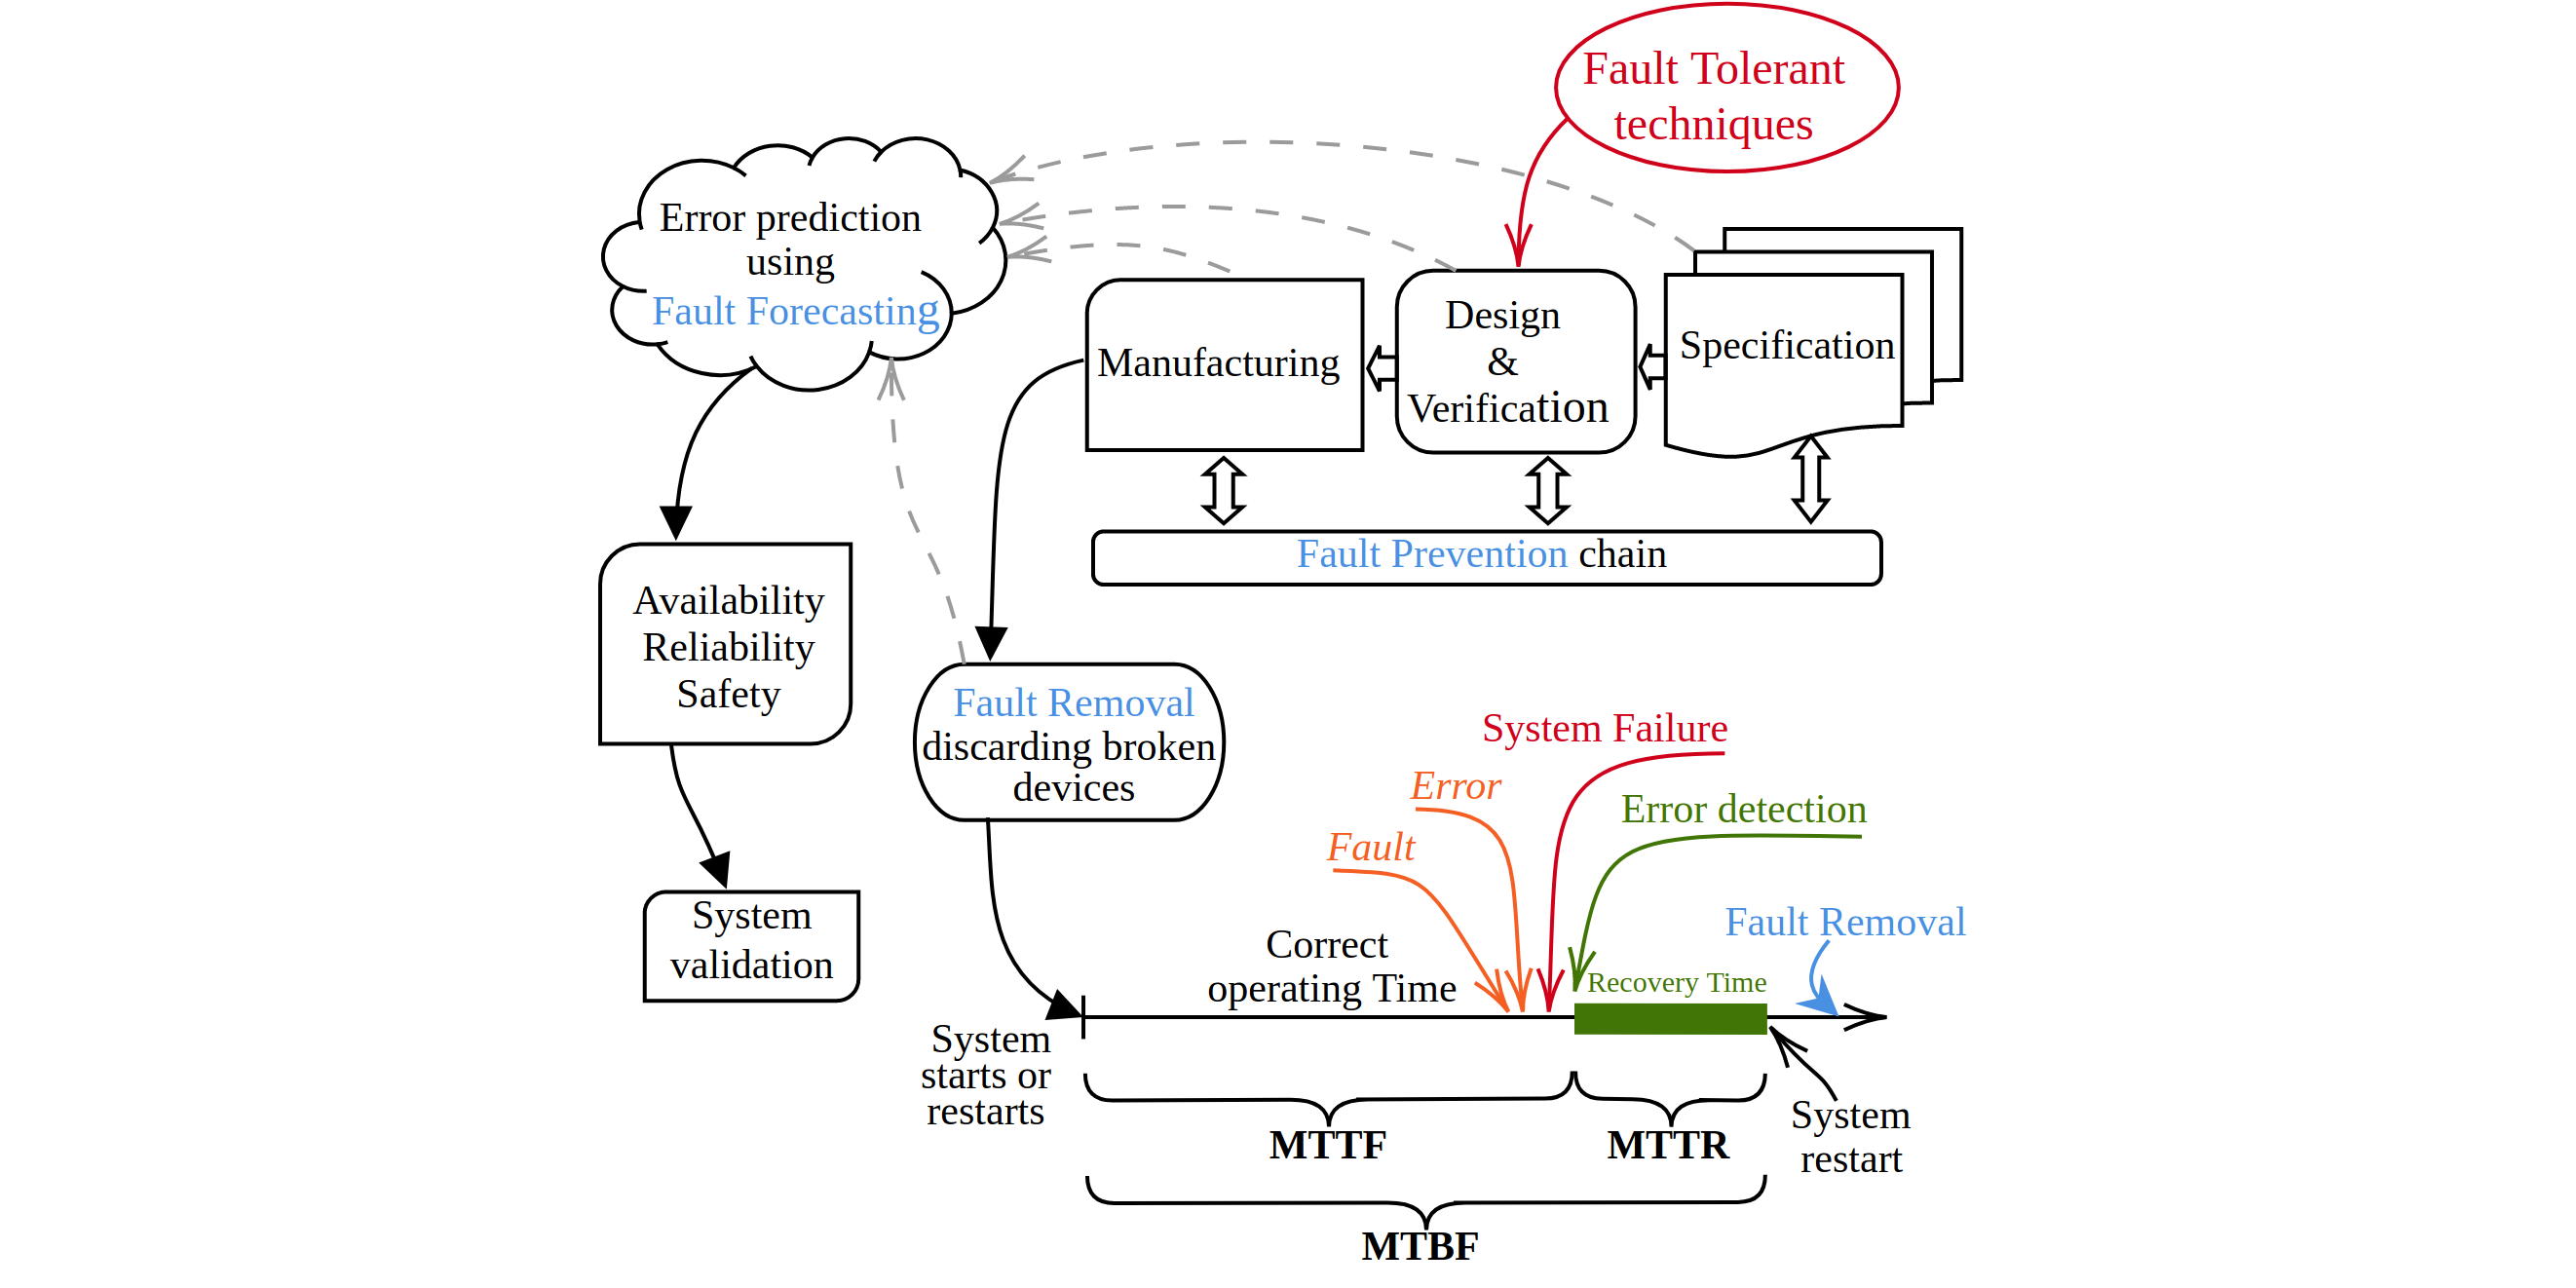
\includegraphics[scale=0.26,center]{./images/Dependability1.png}
				\caption{Design and life of a Dependable System}
				\label{fig:dependability1}
			\end{figure} 
			The block diagram in Figure \figref{fig:dependability1} start with the specification of the system, then the designer use Fault tolerant techniques to design and verify the system, finally the product is manufactured, in these tree steps is applied Fault Prevention in order to reduce unwanted errors. 
			
			After manufacture, the manufacturer apply a selection in order to discard broken devices and finally the systems is sold and it begins to be used.
			Meanwhile we gather data from all production chain in order to use Fault Forecasting to predict MTTF,MTTR and MTBF. Then using predicted data are evaluated required Dependability Attributes and finally system is validated and can be sold.\\
			
			When the system begins to be used there are some periods of correct operations (estimated as MTTF), then at a certain instant a fault occur, this fault can propagate in an Error and this can became a System Failure.
			If the Failure is detected the system begins the Recovery Time ( estimated as the MTTR ) in which the failure is fixed. In the diagram we select a time interval in which fault is propagated but in a Dependable system this should happen rarely. 
			It is also indicated the removal of defected parts using Fault Removal, this techniques can be also applied during Recovery time.  \\
			     
			In the next section we contextualize this thesis work analyzing the parts of a critical electronic system.
		} % end Dependability Model
	
		\newpage
		\subsection{Electronic system parts}{
		    \label{ElectronicSystemParts}
			% Article & books
			% Chapter 5 of : ECSS Space product assurance
			% 
			This section describe how this Thesis is positioned in a complete dependable electronic system.
			
			In figure \figref{fig:ElectronicSystemParts} we give an example of electronic system, it receives information from \textit{sensors} and it controls some \textit{actuators} according to their specification. 
			
			The circuit is powered by a battery or by power network and this energy should be converted inside the board to be used. For this reason there is a part of the PCB dedicated to \textit{voltage conversion}, this block is composed by analogue and digital components that together create the Power Conversion and Distribution system.
			
			\begin{figure}[H]
				\centering
				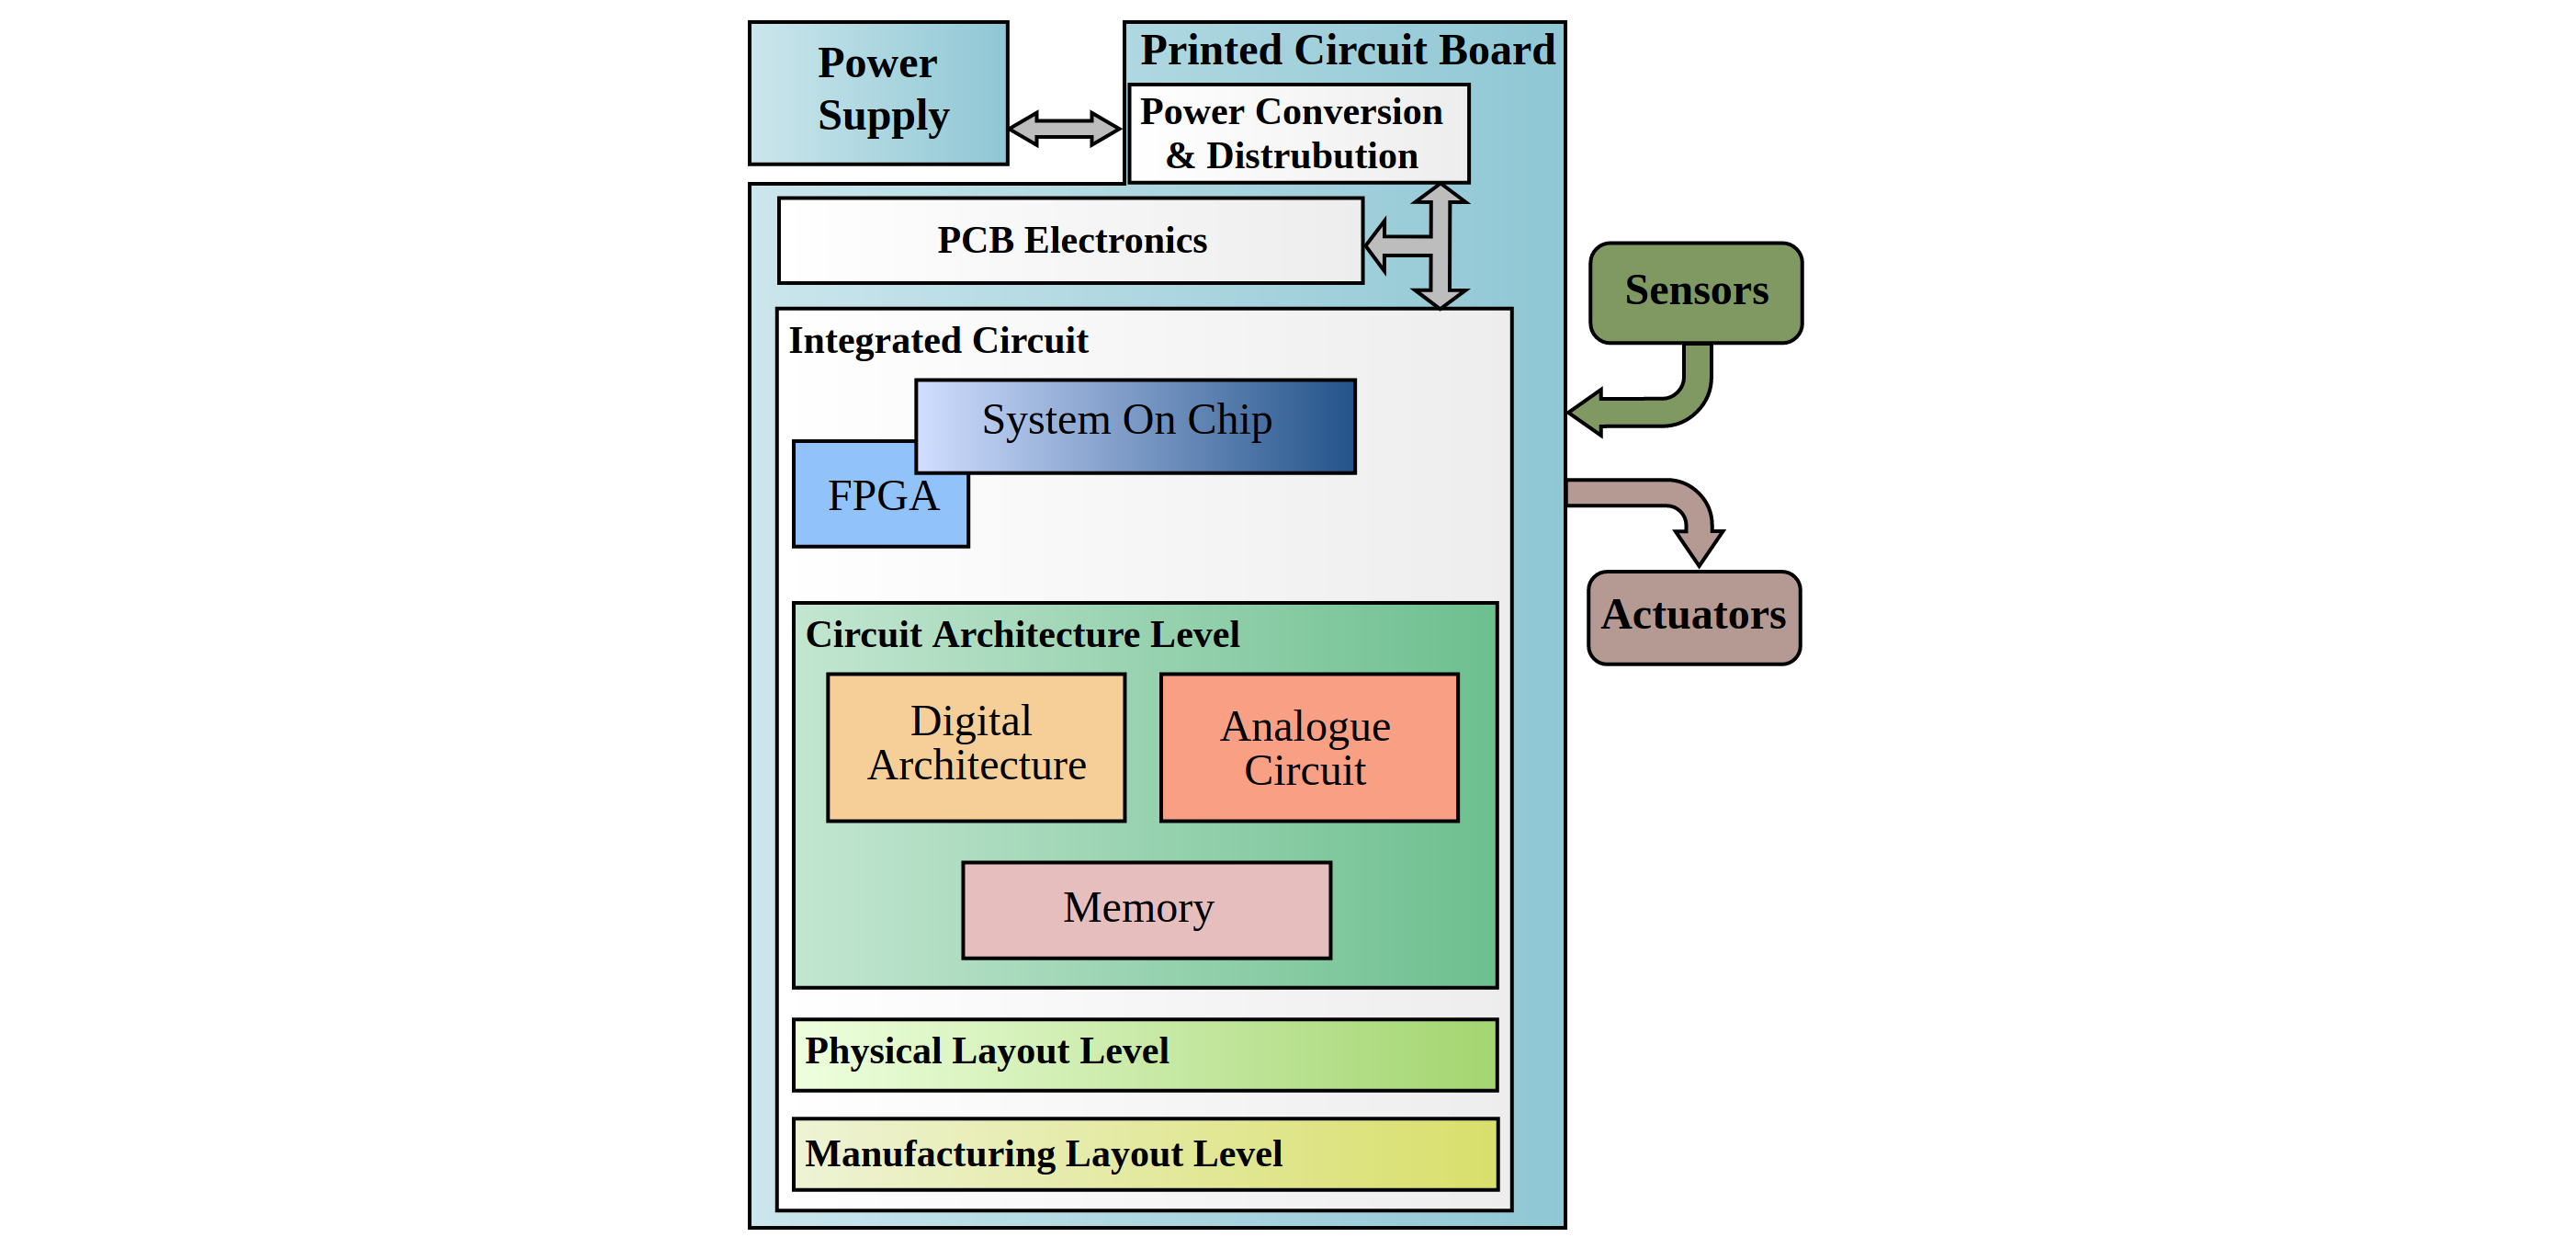
\includegraphics[scale=0.26,center]{./images/ElectronicSystemParts.png}
				\caption{Example of Electronic System}
				\label{fig:ElectronicSystemParts}
			\end{figure} 
			
			The elaboration part instead is composed by integrated circuits that analyze the data received from analog and digital sensors and they use this data to decide how to control the actuators. This elaboration is done by a microcontroller or an FPGA and the design of these ICs have four main design level \bscite{ECSS2016} as you can see in Figure \figref{fig:ElectronicSystemParts}:
			\begin{itemize}
				\item \textbf{Manufacturing Process Level } (lev. 4) : This is the level of manufacturing processes, in this step are defined all technique to create the die from a silicon wafer. In the case of hardened chip the manufacturer apply fault tolerant and fault prevention techniques in order to improve system dependability. 
				\item \textbf{Physical Layout Level} (lev. 3) : It is the set of techniques used to place transistors properly. In the case of robust systems the layout is improved in order to decrease the sensitivity of the circuit to radiation.
				\item \textbf{Circuit Architecture Level } (lev. 2) : At this level circuits design is carried out at the RTL level; the circuits may be digital, analogue or a mixed signal. Generally to make this level robust are used fault tolerance redundancy and error correction techniques.   
				\item \textbf{Electronic System Level } (lev. 1) : In this case we can still work at the RTL level using components previously created at the architectural level, or at the unit level (e.g. cluser computers). In the case of robust systems is used processor redundancy (e.g. lockstep technique) or redundancy of computers.
			\end{itemize}  
		
		
			As we have seen, an electronic system is made up of many parts which must all be dependable in order to have a dependable system. \textit{This Master Thesis will deal with the second design level, which is the architectural one}. 
			In order to be able to use the proposed rtl project correctly, it is necessary to use hardening techniques in all the lower and higher levels. 
			
			In fact what is important for the final application is the dependability of the system, so it would be almost useless to use a hardened processor in a device where the power supply part is not dependable.
			
			Anyway this consideration should be done case by case by designers. 
		
		} % end Electronic system parts
		\newpage
		\subsection{IEC61508 and ISO26262 Standard}{
			% Article & books
			% articolo: iec61508_overview
			% documenti dello standard
			%\lipsum[1-2]
			In 1971 Intel produce the first microprocessors and after only ten years the decreasing cost of processors made possible the spread of electronic devices. In only ten year an huge amount of consumer devices was computerized but the first critical use of electronic devices was in machinery, industrial plant and robots, for these reason in 1985 was born the IEC61508 standard created by a IEC technical task forces created by the International Electrotechnical Commission Advisor Committee Of Safety (IEC ACOS), in order to create a guideline for those industries that needs to meet some safety requirements.\\
	
	        The IEC ACOS is the committee which manages all Technical Committee of IEC and it reports directly to Standardization Management Board (SMB).\\
	        
		    Despite some criticism the IEC61508 began to be used in many industries and it evolves in other more specific standards such as IEC61511 for process industries, IEC62061 for machinery safety ,  IEC61513 for nuclear plants and many others. Today IEC61508 is used manly in machinery, chemical plants, nuclear plants and robots, instead for all on-road vehicles or the so called Automotive world is used the ISO26262 created by the International Organization for Standardization.\\
		    
		    
		    IEC61508 is composed by seven parts and published with the title \textit{Functional safety of electrical/electronic/programmable electronic safety-related systems}, for this reason the standards refers to any devices from electronic valves, relays, and switches to industrial PLC that need to have a certain safety level.
		    
		    To fulfill this safety level the designers needs to reach the \textit{Functional Safety}, It is the full program to ensures that the safety-related E/E/PE system brings to a safety state when a safety issues occurs. Functional safety is a really important concept that is also used in ISO26262 and any following safety-critical standards.
		    
		    As already mentioned IEC61508 is composed by seven parts, each part corresponds has it related document:
		    \begin{itemize}
		        \item \textbf{Part 1:} This part covers General Requirements for compliance with the standards, here are defined Safety Integrity Levels and the overall Safety Life cycle of the system. It is composed by 68 pages.
		        \item \textbf{Part 2:} This part covers requirements for E/E/PE system related systems. It is composed by 96 pages.
		        \item \textbf{Part 3:} This part covers Software requirements for compliance with the standards. It is composed by 118 pages.
		        \item \textbf{Part 4:} This part covers definitions and abbreviations. It is composed by 42 pages.
		        \item \textbf{Part 5:} This part contains many example of methods for the determination of Safety Integrity Levels. It is composed by 54 pages.
		        \item \textbf{Part 6:} This part contains some guidelines on the application of IEC61508 part 2 and IEC61508 part 3. It is composed by  118 pages.
		        \item \textbf{Part 7:} This part contains an overview of techniques and measures in order to support the application of the standard. It is composed by 150 pages.
		    \end{itemize}
		    
		    
		    \subsubsection{IEC61508 part one} {
		    The first part is about the \textbf{General Requirements}, this part is the introduction to the standards and it could be divided in some parts or arguments:
		    \begin{itemize}
		        \item \textbf{Scope:} As already mentioned IEC61508 refers to any E/E/PE devices, these include electro-mechanical devices, solid-state non programmable electronics and and electronic devices based on computer technology ( microprocessors, micro-controller, programmable controllers, ASIC, PLC , smart sensors, transmitters, actuators and so on). 
		        Anyway the standard doesn't cover E/E/PE system which with a System Integrity level lower then 1 or an availability lower the 90\% of time.
		        \item \textbf{Conformance:} In order to be compliance to the standards the designers should create a documentation in which is explained how each requirement is fulfilled according to the decided Integrity level. The documentation required is usually considerable and you should be detailed in fulfilling the requirements.
		        \item \textbf{Documentation: } The main argument of the documentation is the Safety Life Cycle which represent the life of the product from specifications to decommissioning. This life cycle should be described in order to enable the Functional Safety verification and assessment, documentation also should be a support for the life cycle process in order to guarantee that each step is executed.
		        \item \textbf{Management of functional safety: } Functional safety should be achieved and maintained, for these reason you should write all activity that make this possible in a document called Functional Safety Management (FSM) plan. This plan should contain all strategy used, all people responsible of safety , all about Safety Life Cycle and Functional Safety, the procedures to ensure that the personals are competent and to enable the analysis of hazardous incidents,the maintenance operations, the procedures to change something in the system and some other minor documentations. 
		        It is also very important that each Safety Life Cycle part should have a responsible for that phase.
		        \item \textbf{Safety Life Cycle Requirements: } Safety life cycle is a closed loop in which the system goes through identification, analysis, design and verification. This life cycle came from the analysis of the Health Safety Executive (HSE) about the industrial control systems classified accident causes shown in figure \ref{fig:HSEResultsOfSystemFailureCauseStudy}.
		        
		        \begin{figure}[H]
    				\centering
    				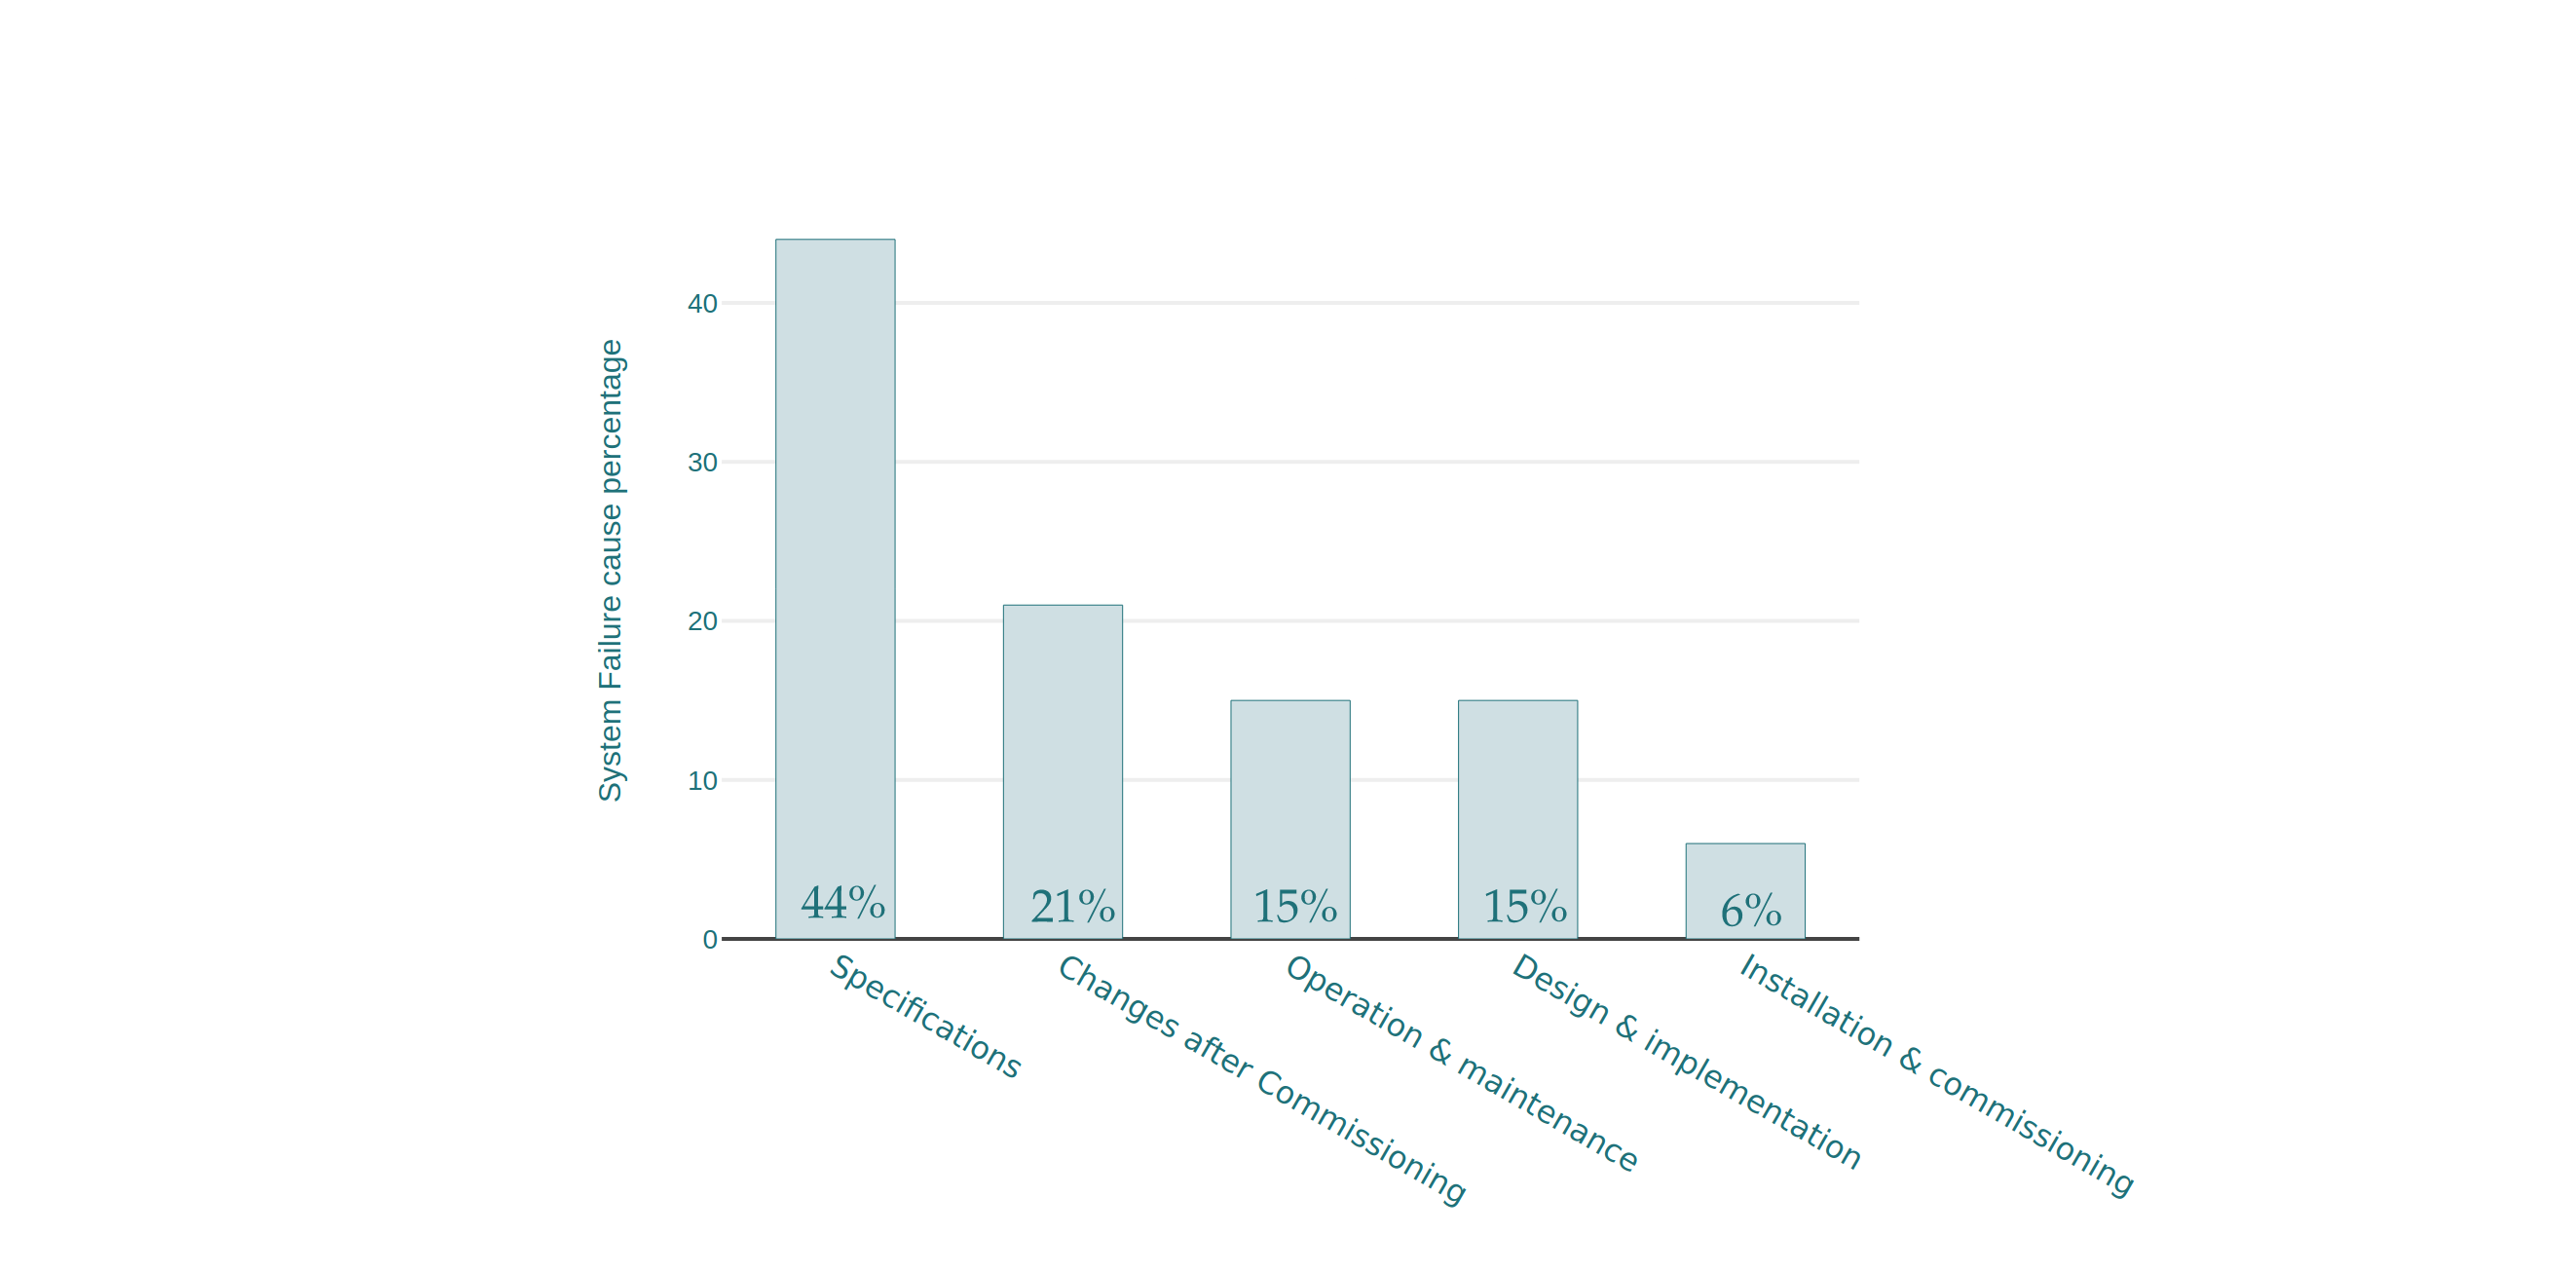
\includegraphics[scale=0.22,center]{./images/HSEResultsOfSystemFailureCauseStudy.png}
    				\caption{Results of system failure cause study from HSE}
			    	\label{fig:HSEResultsOfSystemFailureCauseStudy}
			    \end{figure} 
			    
			    In figure \ref{fig:HSEResultsOfSystemFailureCauseStudy} there is the overall  safety life cycle of a safety-critical system composed by E/E/PE device and software, this is the life cycle to follow the system should accomplish to the IEC61508 standard. The block diagram in figure \ref{fig:HSEResultsOfSystemFailureCauseStudy} is only a brief summary of the sagfety life cycle, in order to completely understand this part read the IEC61508 part one clause 7.
	                
			    
			    \item \textbf{Safety Integrity Level:} IEC61508 define four level of Safety Integrity Level, they are the order of magnitude levels of risk reduction. The SIL is defined by two table, a table of Low Demand Mode \ref{fig:SIL_DemandMode} of operation and Continuous mode of operation \ref{fig:SIL_ContinuousMode}. When a system work in Low Demand mode the safety function is executed only when it is needed, otherwise in Continuous Mode of operation the safety function is executed continuously. For these reason when the safety function is in Continuous mode the SIL is calculated as failure per hour, instead when the safety function work in Low Demand Mode the SIL is calculated as dangerous failure on demand.
			    
			    \begin{figure}[H]
    				\centering
    				
\includegraphics[scale=0.2,center]{./images/SIL_ContinuousMode.png}
    				\caption{SIL definition for continuous mode}
			    	\label{fig:SIL_ContinuousMode}
			    \end{figure} 
			    \begin{figure}[H]
    				\centering
    				
\includegraphics[scale=0.2,center]{./images/SIL_DirectMode.png}
    				\caption{SIL definition for demand mode}
			    	\label{fig:SIL_DemandMode}
			    \end{figure}
			    Looking at the table you should notice that continuous mode seems to have lower value of probability for the same SIL, anyway we should consider that  SIL is evaluated in one year for definition and that the continuous mode probability is referred to failure per hour. For these reason and considering that there are 8760 hour in one year, the two SIL table are comparable in terms of safety metric.
			    
			    \item \textbf{Functional Safety Assessment:} Basing on the Safety Integrity Level the failure in the system could cause a certain amount of injury. For this reason the standard states that there should be independent person, department or organization that do a Functional Safety Assessment of the system. 
			    
			    This naturally increase the safety of the final system since this procedure is a redundancy in verification. The people who apply the Functional Safety Assessment should be competent and they will have the responsibility of the system.
		    \end{itemize}
		    
			   \begin{figure}[H]
    				\centering
    				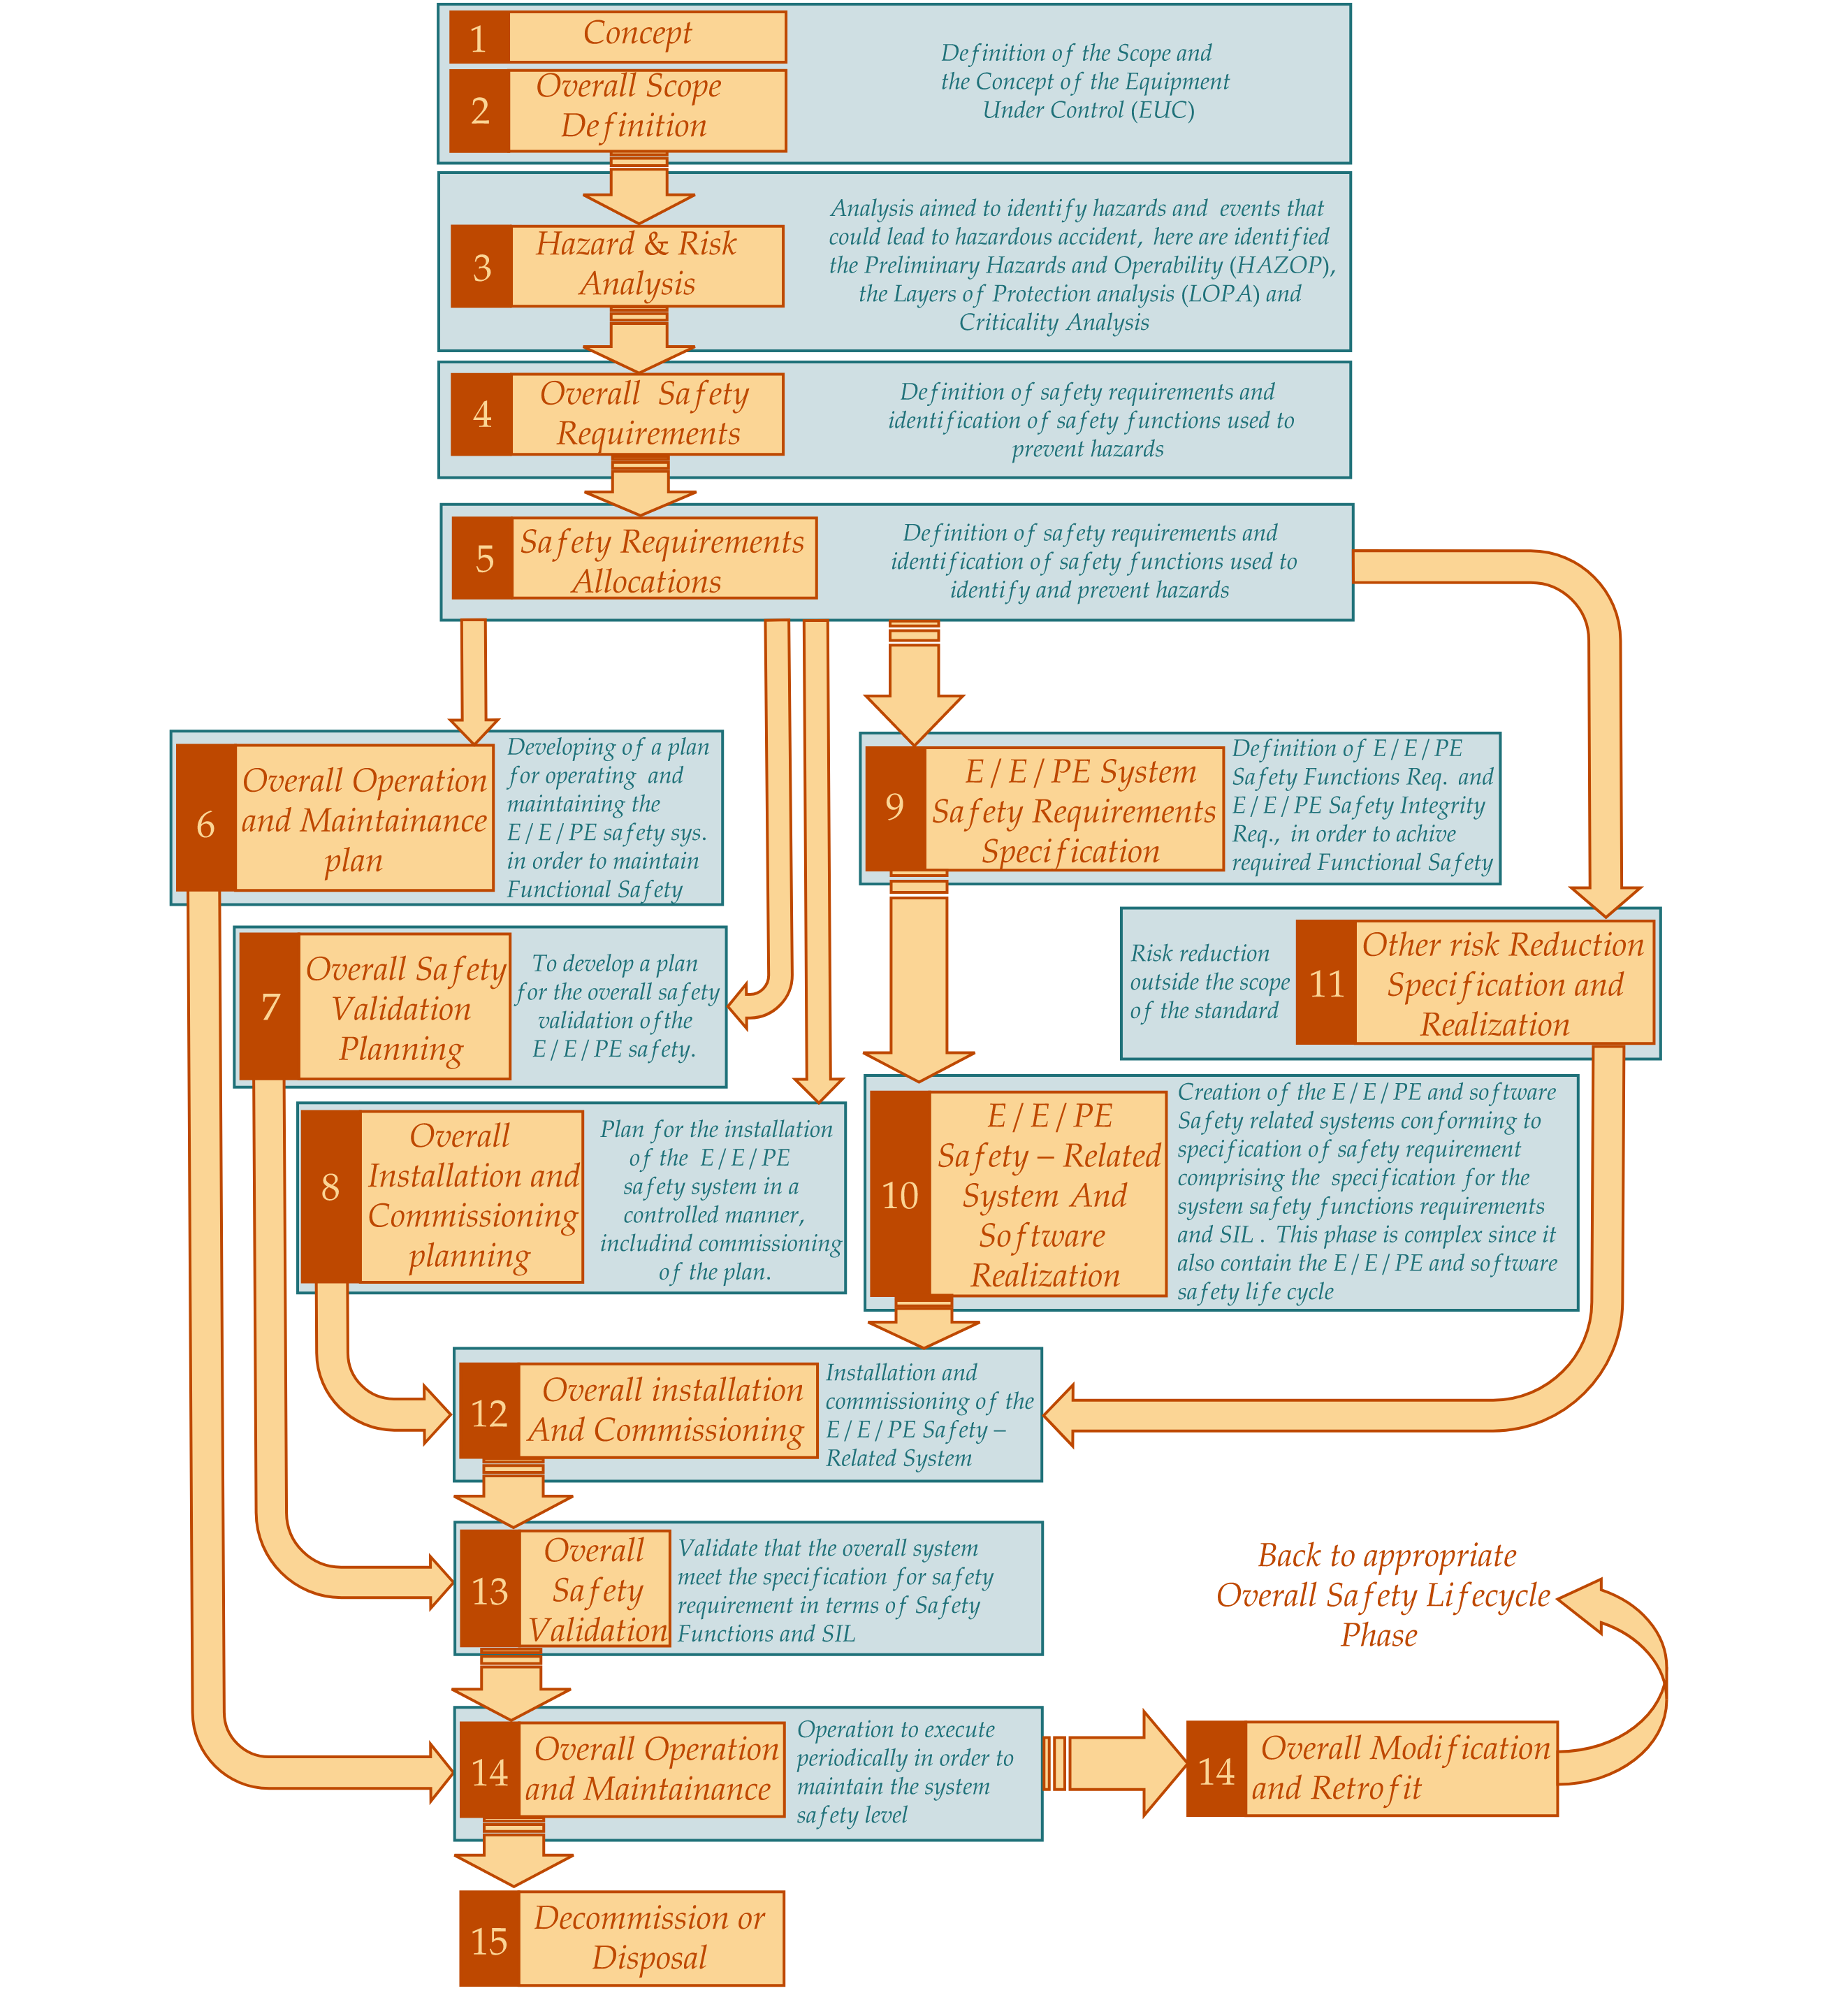
\includegraphics[scale=0.2,center]{./images/SafetyLifeCycle.png}
    				\caption{Overall Safety Life Cycle}
			    	\label{fig:FirstPartOfSafetyLifeCycle}
			    \end{figure} 
		    
		    }
		    \subsubsection{IEC61508 Part two Hardware Requirements} {
		        Part two of IEC61508 covers the requirements of safety-related hardware. In particular this part discusses and expands phase 9 of the main safety life cycle (figure \ref{fig:FirstPartOfSafetyLifeCycle}).
		        
		        Inside this part is described the methods used to determine the SIL for a safety-related system. In order to understands this procedure we should define some terms:
		        \begin{itemize}
		            \item \textbf{Safe Failure Fraction (SFF):} From part 4 of IEC61508 it is defined as "property of a safety related element that is defined by the ratio of the average failure rates of safe plus dangerous detected failures and safe plus dangerous failures". The "safe plus dangerous failures" is the overall number of failure, since in this thesis we will work with fault injection this number is the number of fault injected.
		            
		            Instead "average failure rates of safe plus dangerous detected failures" are the overall number of failure injected that don't cause an error in the output of the stage. For these reason in this thesis:
		            \[ SFF = 1 - \frac{\text{Errors at the output of our stage}}{\text{Total injected error}}\]
		            \item \textbf{Element Type:} It is a classification of the elements used in the system, for the standard exist two type of element, Type A and Type B. Element Type A: they have well defined failure modes and they have failure behaviour completely determined and "there is sufficient dependable failure data to show that the claimed rates of failure for detected and undetected dangerous failures are met". 
		            
		            
		            For these reason Type A are those element which are enough simple to be completely defined and which behaviour is predictable. 
		            Element Type B: They have not well defined failure mode or they haven't failure behaviour completely defined or "there is insufficient dependable failure data to support claims for rates of failure for detected and undetected dangerous failures". 
		            
		            
		            Therefore Type B are usually complex elements which general behaviour is not completely predictable, anyway it is important to notice that for Type A is used "and" statement instead is used "or" statement for Type B, for these reasons it is more common to have a Type B element rather than a Type A, for our scope ASICs can be defined as Type B since not all event inside the chip can be modeled in order to predict failure behaviour.
		            \item \textbf{Hardware Fault Tolerance (HFT):} From part 2 of IEC61508 it is defined as: "HFT of N means that N+1 is the minimum number of faults that could cause a loss of the safety function", This means that in a system with HTF equal to 1  we need at least two fault to cause a loss in the safety function. So a system with HFT of one is designed to tolerate only one dangerous failure, in this thesis we use triplication that is a way to create a system with HTF of one.
		        \end{itemize}
		        
		        
		        In order to claim a certain level of SIL we should follow \textbf{Route $1_H$} or \textbf{Route $2_H$} explained in the coming paragraph.
		        \paragraph{Route $1_H$}{
		            This approach takes in consideration the Safe Failure Fraction (SFF) of the elements. Route $1_H$ starts from the calculation of SFF and from the required SIL we find the required HFT. This connection between SFF, SIL and HFT change from Type A and Type B as we can see in Table \ref{fig:TypeASIL} for Type A and in Table  \ref{fig:TypeBSIL} for Type B.
		            \begin{figure}[H]
        				\centering
        				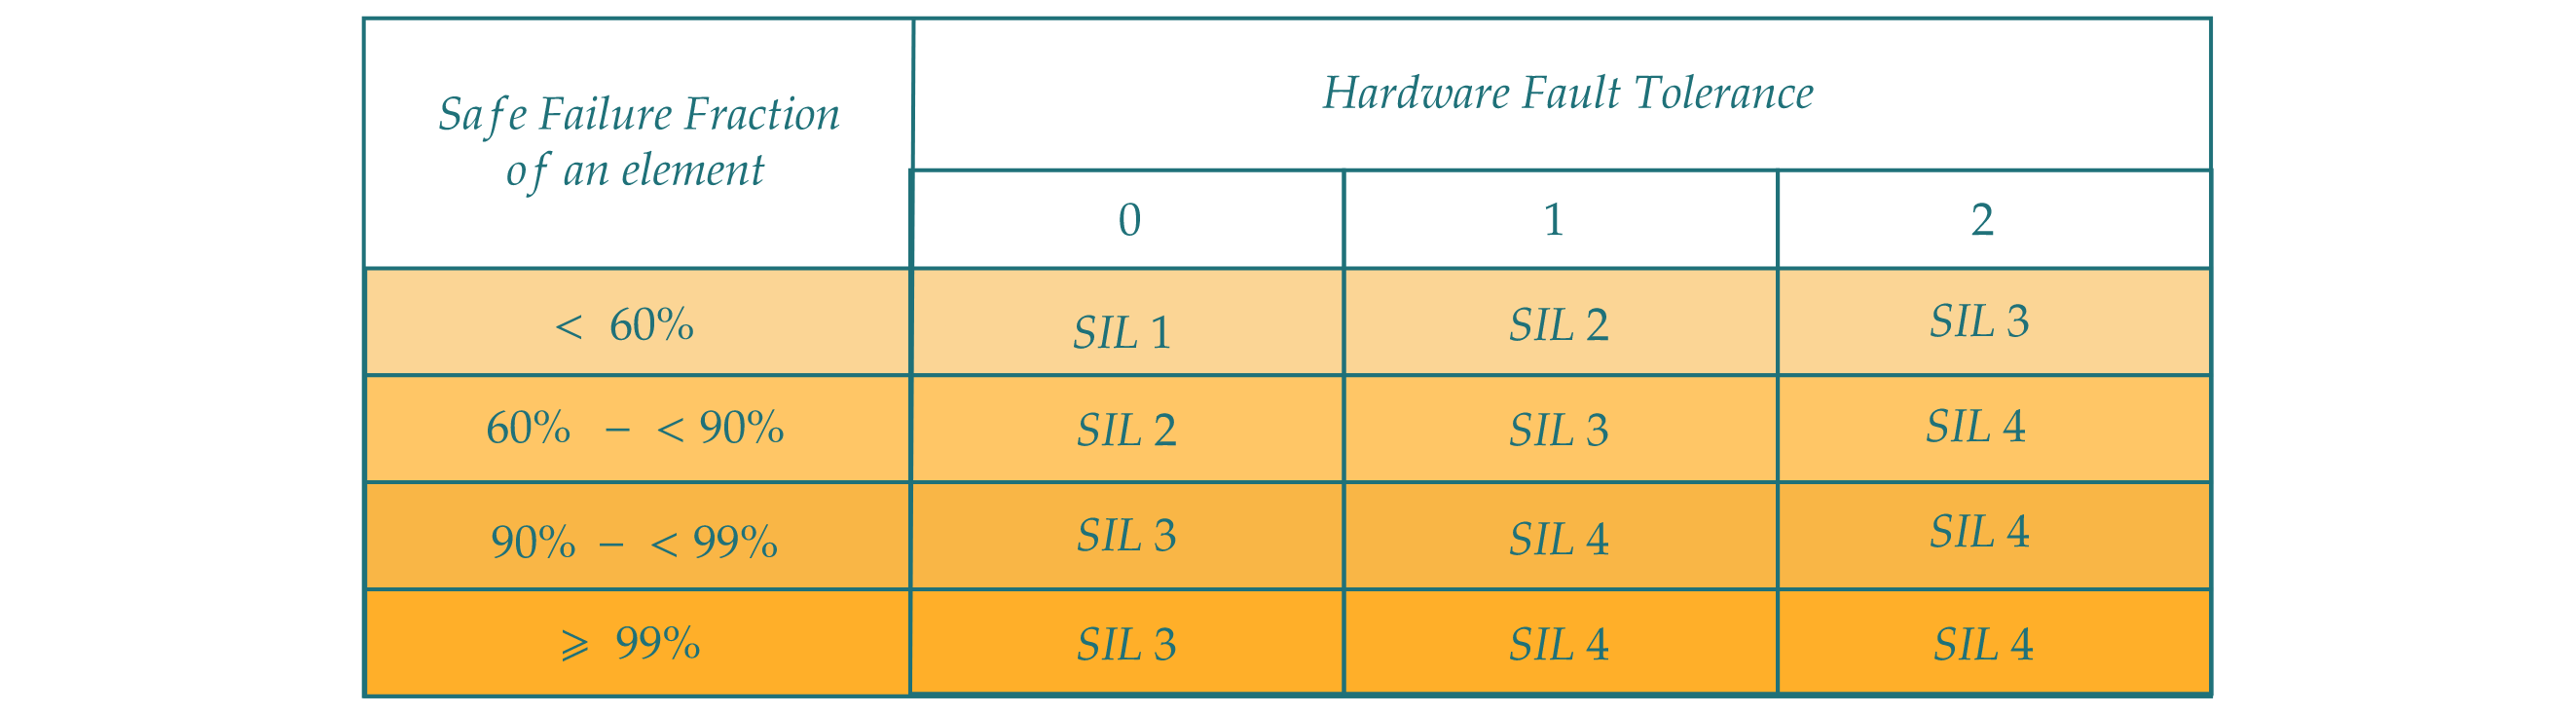
\includegraphics[scale=0.2,center]{./images/TypeASILTable.png}
        				\caption{Maximum SIL for a safety function carried out by a type A element.}
    			    	\label{fig:TypeASIL}
    			    \end{figure} 
		            \begin{figure}[H]
        				\centering
        				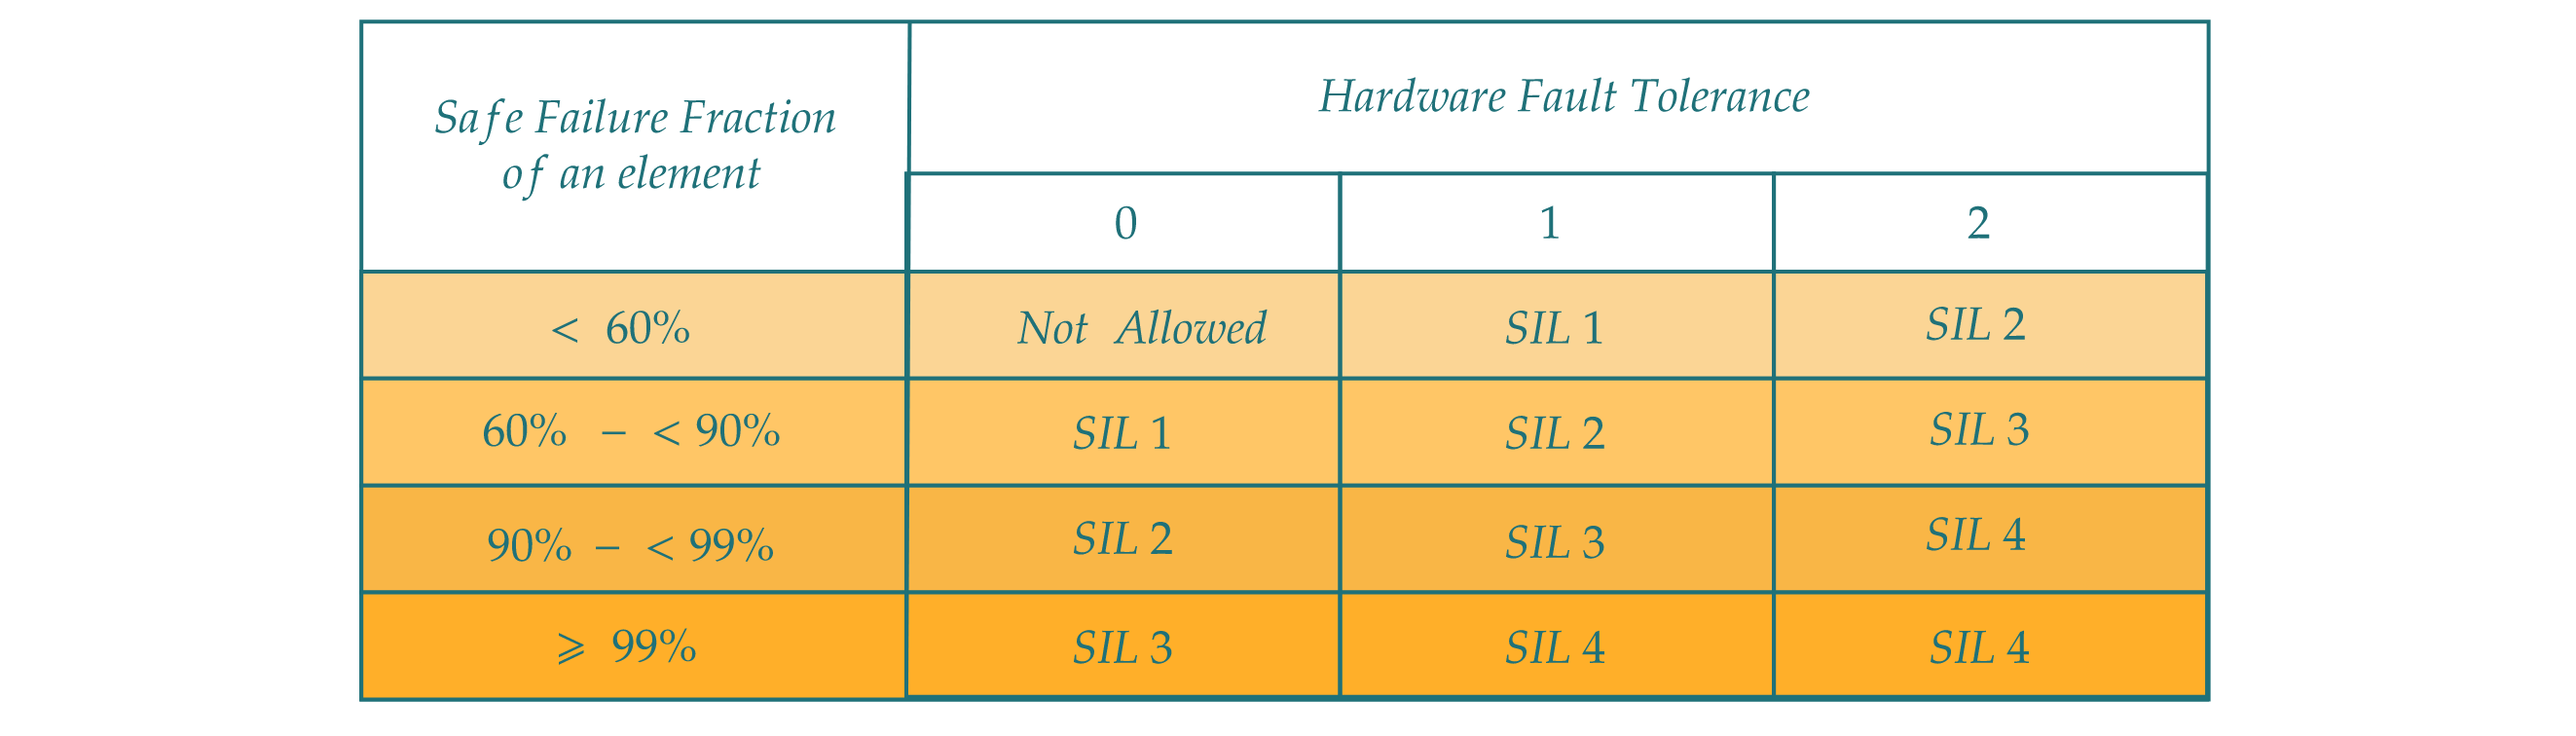
\includegraphics[scale=0.2,center]{./images/TypeBSILTable.png}
        				\caption{Maximum SIL for a safety function carried out by a type B element.}
    			    	\label{fig:TypeBSIL}
    			    \end{figure} 
    			    
		        }
		        \paragraph{Route $2_H$}{
		               Route $2_H$ don't consider the SFF of a system but only specify the level of Hardware Fault Tolerance according to required SIL and the operation mode.
		               
		               
		        }
		        
		        
		    }
		    
		    \subsubsection{ISO26262}{
		            ISO26262 is the standard used in Automotive Industries and in whatever device that should be used in on-road vehicles. It is born in order to answer to the increasing amount of safety-related electronic used in vehicles, for these reason it has been created much later IEC61508, in 2011.
		            
		            This standard is radically different from the IEC61508. Anyway ISO26262 was created after the IEC61508 and so many aspect of the two standards can be connected, for example the Safety Integrity Level in ISO26262 is replaced with Automotive Safety Level (ASIL). A complete analysis of ISO26262 is outside the scope of this thesis, anyway the use of the designed architecture in Automotive field tipically imply an ISO26262 certification.
		    }
		    
		} % end IEC61508 Standard
	}% end Safety critical application system
	\newpage
	\section{Dependability of Integrated Circuits}{
		% Article & books
		% Case study in chapter 8 of : (book) Fault tolerant Systems
		% Architecture design for soft errors -> intro: Evidence of Soft Errors
		Faults in integrated circuits are due to both bit flip or electrical problems such as broken interconnects. The origins of these problems are due both to the aging of integrated transistors and their susceptibility to charge injection by external particles, such as cosmic rays.\\
		
		
		These two phenomena are influenced by the field of use of the IC and by the working conditions. For example, aging is accelerated by high temperatures and high workloads, which wear out the interconnections. On the other hand the influence of external particles increases in space applications due to the increased cosmic ray flux, as well as in nuclear power plants or where some radioactive materials are present.\\
		
		
		\textit{The understanding of these phenomena is essential to improve fault tolerance techniques applied to integrated circuits also at RTL level in different application}, therefore the causes and mechanisms of faults are now investigated by dividing them into \textit{internal factors} (graceful degradation) and \textit{external factors} (e.g. particle flux).
		
		\subsection{Internal Factors of Faults}{
			% Article & books
			% intro of: (book) Fault Tolerant Computer Architecture
			% Chapter 2 of : (book) Fault tolerant Systems
			% Defect Tolerance in VLSI Circuits chapter 10 of : (book) Fault tolerant Systems
			% Cyber-Physical System Chapter 7 of : (book) Fault tolerant Systems
			% Introduction (for cosmic rays) : Fault‐Tolerance Techniques for Spacecraft Control Computers
			% Radiation Effects in a Post-Moore World
			As already mentioned, the internal factors of faults are due to intrinsic electrical problems of transistors, which can be caused either by the \textit{breakage of the interconnections} or by problems related to the \textit{gate oxide failure}.
			
			As far as \textit{interconnections} are concerned, there are two origins of failure:
			\begin{itemize}
				\item \textbf{Electromigration} (EM) : EM is a phenomenon known since 1966 \bscite{EM1989}, whereby the electrons generating the electric current in the interconnections impart a momentum to the atoms of metal. This momentum transfer can create void in the very small interconnections of ICs. The phenomenon is directly proportional to the square of the charge density ($j_e;\;\; [A/cm^2]$) and depends exponentially on the \textit{activation energy} of the material ($E_a;\;\;[eV]$) and on the temperature ($T \;\;\;[K]$). These relationship are condensed in the Median Time To Failure calculated according to the Black's formula \bscite{Mukherjee2008}:	
				\begin{equation}
					MeTTF_{system} \;=\; \frac{A_0}{j_e^2}\,e^{\frac{E_a}{kT}} 
				\end{equation}
				Where $A_0$ is a technology dependent constant and k is the Boltzmann constant. 
				
				The opposite effect to EM is due to mechanical stress which tends to compensate for the displacement of metal atoms, this principle is the basis of the Blech effect for which below a certain length (called the Blech length) EM has no effect because the two forces are balanced.
				
				Normally the length of the interconnections is greater than the Blech length and for this reason EM should be reduced by various techniques. Two of these techniques are the use of metal alloys (Al+Cu, Al+Pd) or the creation of \textit{Bamboo Structures} that reduce the number of metal grains. In fact, the creation of a void in a connection starts at the interface between two or more grains of metal. Here the mobility of the atoms is greater respect to normal mobility, for this reason metal atoms are able to move  and they leads to an avalanche effect which creates the final voids.	\\
				
				Electromigration create both permanent or intermittent faults and leads the chip in the wear-out phase. as we have seen this phenomena is related to current density that normally depends on workload, hence architecture and system fault tolerant strategy for EM reduction lead with resource multiplexing and oversizing.
				
				\item \textbf{Metal Stress Voiding} (MSV) :  The MSV is due to the difference in expansion ratios between the metal of the interconnection and the surrounding material. The phenomenon is closely related to temperature and the formula \figref{MTTF_MSV} gives a quantitative evaluation in terms of MTTF \bscite{Mukherjee2008}:
				\begin{equation} \label{MTTF_MSV}
					MTTF_{system} \;=\; \frac{B_0}{(T_0-T)^n}\;e^{\frac{E_b}{kT}} 
				\end{equation}
				Where:  $B_0$, $n$ and $E_b$ are material dependent constants, k is the Boltzmann constant and T is the temperature in Kelvin. According to the equation the larger the temperature the lower the MTTF, this is a further reason why heat dissipation is important for system dependability. Another important methods to reduce the influence of this phenomenon is the use of stronger metals, with expansion constants similar to the interfaces.

				MSV related faults are very similar to those caused by EM and can be either intermittent or permanent.
			\end{itemize}
		
			
			As far as \textit{Gate Oxide Failure} is concerned, there are three main physical mechanisms that cause faults:
			\begin{itemize}
				\item \textbf{Negative Bias Time Instability} (NBTI) : NBTI is the process that causes short-channel pMOS (hence the term Negative Bias) subjected to high temperature or negative gate voltages, to degrade the maximum frequency of the circuit and to create faults. These phenomena is due to charges being trapped under the gate of the pMOS \bscite{Mukherjee2008} \bscite{FTS2021}.
				These charges slow down the switching process, decreasing the speed of the circuit and creating Timing Faults. Timing Faults happen when the propagation time of the critical paths no longer respects the sampling conditions according to the circuit's clock. \\
				
				The physical effect related to this phenomenon is the decrease in mobility under the gate due to the bombardment of charges during normal operations. This causes the pMOS threshold voltage to increase (hence the term instability) and the maximum current to decrease, leading the logic gates (which use pMOS) to slow down and fault \bscite{Mukherjee2008}.\\
				
				To reduce the contribution of this effect are used Dynamic Voltage Scaling and the power gating \bscite{FTS2021}.
				
				\item \textbf{Hot Carrier Injection} (HCI) : HCI leads to a reduction of the $f_{max}$ of the circuit but in this case  this is due to the charges trapped in the gate. In fact, during the acceleration along the channel, the ionization effect produces electron-hole pairs, if these charges have sufficient energy they can inject themselves in the gate and get trapped \bscite{Mukherjee2008}. This creates a variation of the threshold voltage that lead to faults as in the case of NBTI.
				
				Unlike the other effects, HCI get worse at lower temperatures due to the increase in charge mobility in the material. The first consequence of HCI is the degradation of the threshold voltage that decreases the maximum saturation current, this lead to a reduction of the maximum frequency from 1\% to 10\% \bscite{Mukherjee2008}.
				
				Again, duty cycle reduction is a way to reduce the effect of HCI. Despite technological advances, HCI is still present in recent Tri-Gate Nanowire \bscite{HCI_nanowire}, FLASH memories \bscite{HCI_NAND_flash} and general CMOS electronics.
				
				\item \textbf{Time Dependent Dielectric Breakdown} (TDDB) : Continuously applied voltages in the transistors create defects in the gate material, which can lead to the creation of conductive paths between the channel and the gate, knocking out the transistors. In thicker gate this effect is more pronounced.
				
				To reduce this phenomenon, attempts are made to reduce the gate voltage and to use stronger gate materials.
				
			\end{itemize}
			
			
			\begin{wrapfigure}[18]{r}{0cm}
				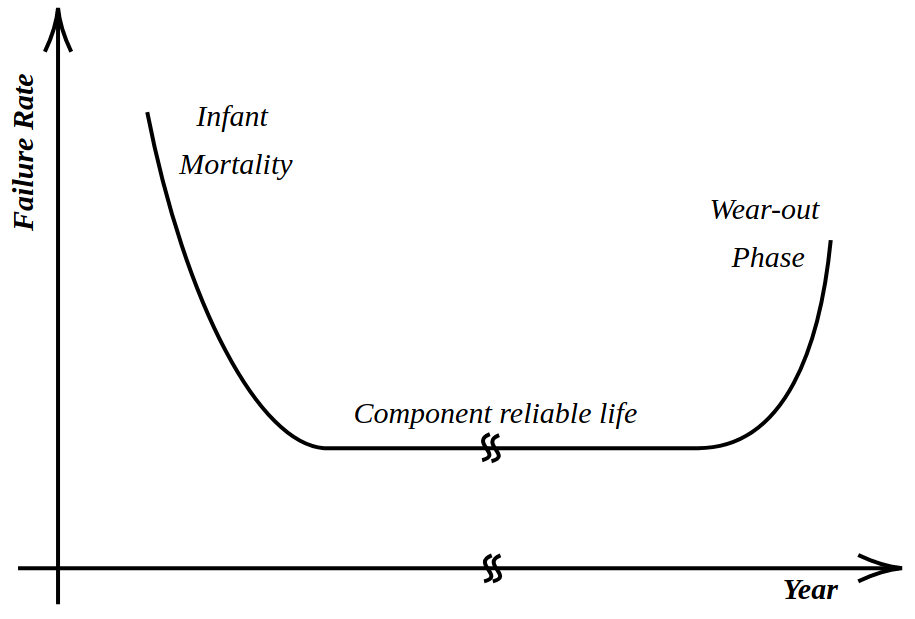
\includegraphics[width=0.5\textwidth]{./images/ComponentLife.png}
				\caption{Example of Electronic System}
				\label{fig:ComponentLife}
			\end{wrapfigure} 
		
		
			All these effects added to the manufacturing defects lead to: an infant mortality phase of the components which are discarded before being sold, a life phase with a certain fixed value of failure rate and finally a wear-out phase which causes the final failure of the integrated circuit. This variation of the failure rate over time is shown in the figure \figref{fig:ComponentLife}.
			\vspace{2cm}
		
		}% edn Internal Factors of faults
		\subsection{External Factors of Faults - Radiations}{
			For External Factors of Faults we mean all those external factors that can cause ICs to malfunction. In the next paragraphs we first analyze the different sources of radiations, and then the radiation effects on ICs.
		
			\subsubsection{Radiation Levels and Sources}{
				%The sources of Alpha and Neutron particles in the atmosphere are the sun and supernovae explosions that generate Solar and Galactic rays respectively. These two types of rays create the \textit{Primary Cosmic Rays}, which are those that reach the surface of the Earth's atmosphere. Contrary to what one might think, Galactic rays are the most energetic primary cosmic rays (typically above 1GeV), with a flux of 36000 particles/$cm^2$ per hour. A simple demonstration of this is that the variation of terrestrial cosmic rays between night and day is only 2\%  \bscite{Mukherjee2008}. Galactic rays consist mainly of protons which decay into other particles when hit the atmosphere .
				
				%The Primary Cosmic Rays collide with particles of the atmosphere and generate the \textit{Secondary Cosmic Rays}, composed mainly of Pions, Muons and Neutrons. The Pions and Muons decay quickly ($1ns /\,1\mu s$), while the Neutrons have an average lifetime of 11 min, so they have time to collide with other atoms and create further particles, these particles descend into the atmosphere to eventually create the \textit{Terrestrial Cosmic Rays}. The secondary cosmic ray fluxes are exponential along the atmosphere, peaking at an altitude of $15 km$. For this reason, aircraft have to use different systems than on the ground to keep the system dependable. In fact, the Terrestrial Cosmic Rays are only 1\% of the Primary ones with an average of 20 Neutrons/($cm^2$ hour).
				
				There are essentially four sources of radiation: supernovae and celestial explosions that create Galactic Cosmic Rays, the Sun that generates Solar Cosmic Rays, terrestrial radioactive materials (e.g. $^{238}U$), and finally nuclear weapons and reactors. The characteristics and radiation levels of these sources are described in the following paragraphs.
				
				
				\paragraph{Galactic Cosmic Rays (GCRs)}{
						In order to understand how GCRs arrive on earth, we need to know the structure of the heliosphere. 
						
						
						As described in \figref{fig:SolarSystemGCRs}, the Sun emits particles in all directions, mainly protons and alpha particles that form the Solar Wind at $400-700km/s$. 
						The Solar System moves through the local interstellar medium (LISM) composed mainly of helium and rarefied hydrogen. 
						For this reason the solar wind collides at supersonic speed with interstellar dust (at a relative velocity of about $26km/s$ respect to the Sun) and is slowed down to subsonic speeds at the so-called 'Termination Shock' (75-100 $AU$ from the Sun). 
						
						After the Termination Shock, moving away from the Sun there is a zone where the LISM and solar rays are compressed to form plasma, this zone is called Heliosheath (pink filled at the right of the sun in \figref{fig:SolarSystemGCRs}). At the end of the Heliosheath there is the limit beyond which the solar rays cannot go, this is called the Heliopause ($\simeq$ 121-150$AU$ from the Sun). Beyond the Heliopause there is probably the Bow Wave, the shock wave of the LISM with the heliosphere, such as water does on the bow of a ship.\\
						
						
						\begin{figure}[H]
							\centering
							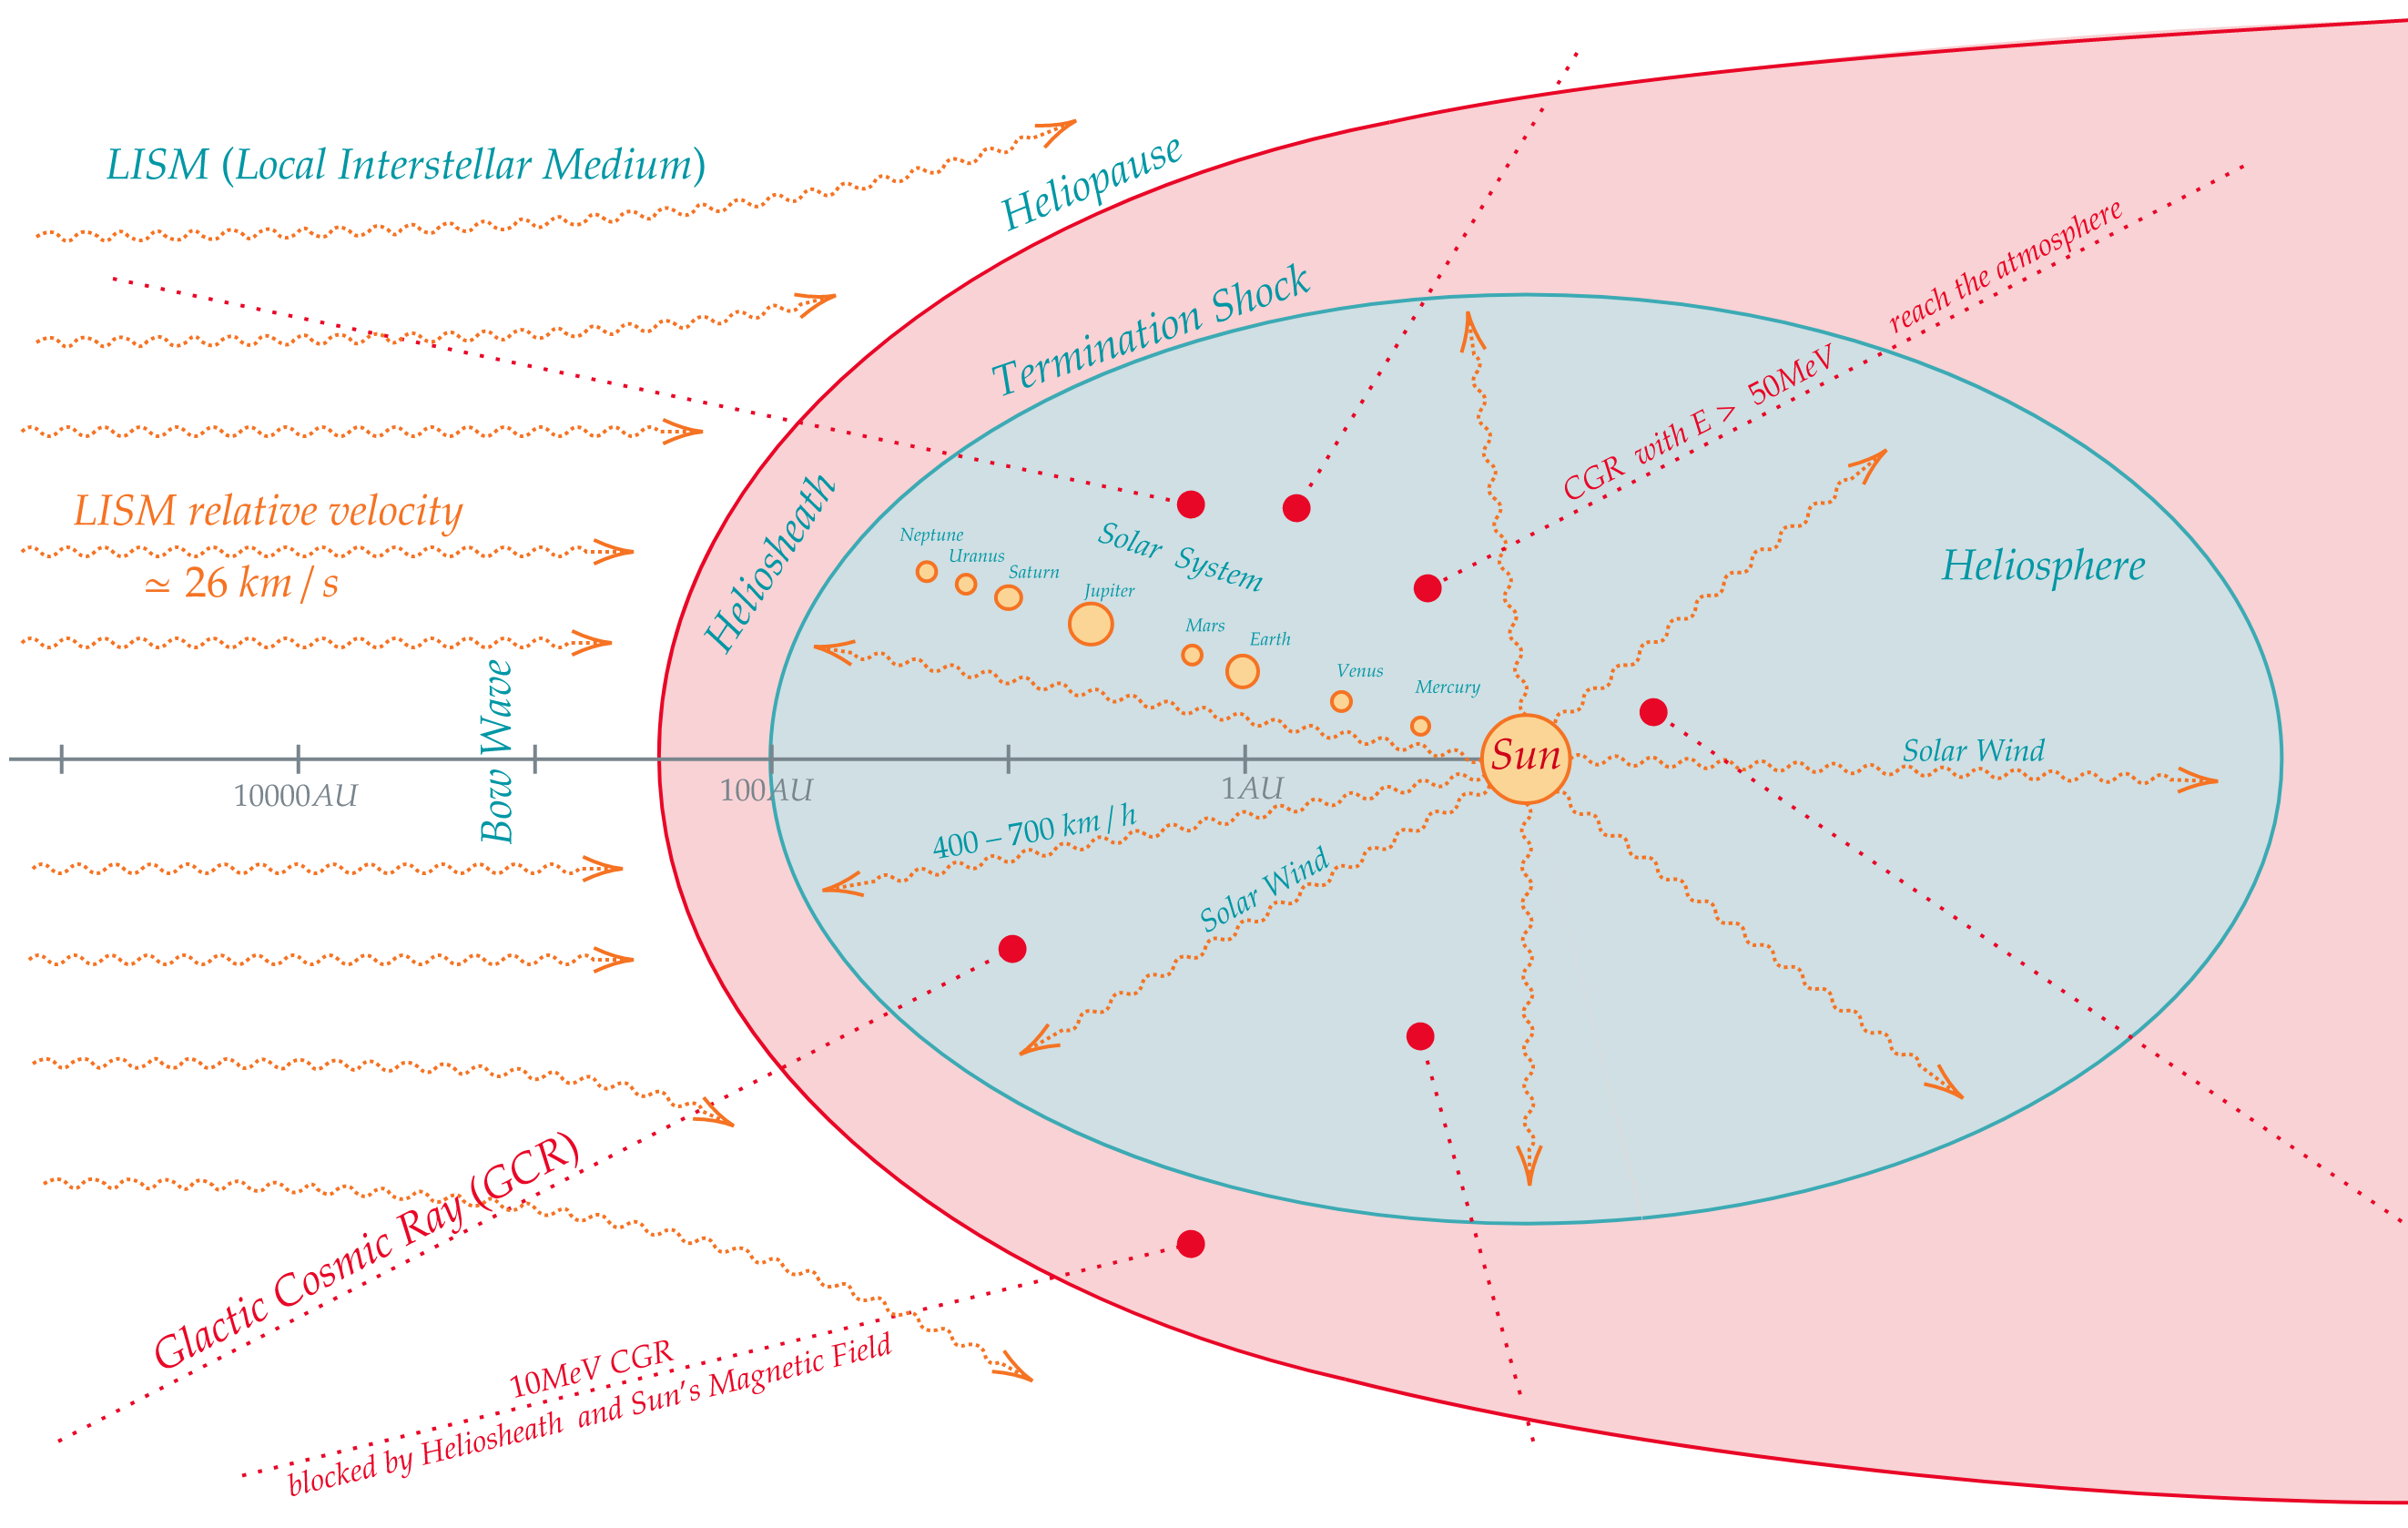
\includegraphics[scale=0.16,center]{./images/SolarSystem_GCRs.png}
							\caption{Solar system moving within the LISM while it is hit by GCRs, the planets are not to scale and the distance is logarithmic.}.
							\label{fig:SolarSystemGCRs}
						\end{figure} 
					
						In this environment, the Galactic Cosmic Rays are the isotropic flow of energetic particles from outside the solar system that try to pass through the solar wind and magnetic field shields into the Earth's atmosphere as shown in \figref{fig:SolarSystemGCRs}. 
						
						GCRs are created by stellar explosions such as supernovae and gamma-ray bursts, active galaxies or quasars, they reach the Earth isotropically and so they hit it uniformly in more or less all directions. 
						In fact, unlike the LISM, these rays have an energy that can reach $100\,000\,TeV = 10^{20}\,eV$. Anyway considering that GCRs need to have an energy of at least $50MeV$ to pass the Termination Shock, only 35\% of them reach the Earth's atmosphere.\\
						
						\newpage 
						\begin{wrapfigure}[22]{r}{0cm}{
								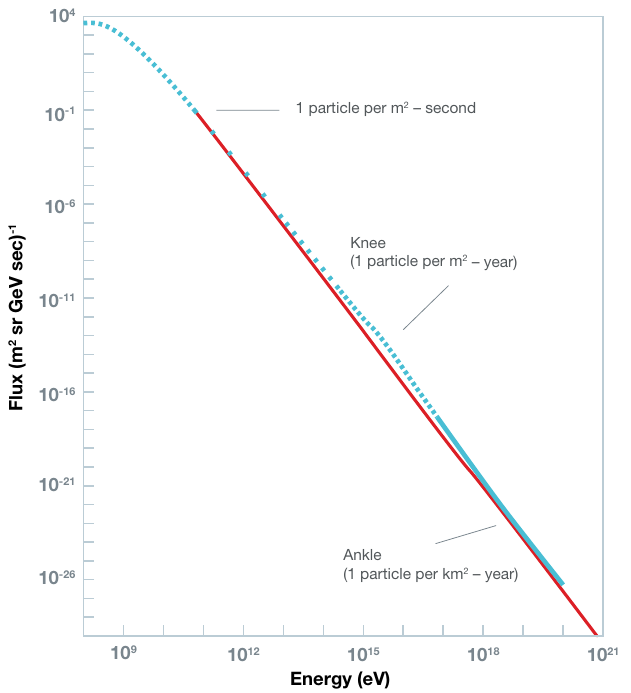
\includegraphics[width=0.5\textwidth]{./images/Flux_of_cosmic_rays.png}
								\caption{Spectrum of Galactic Cosmic Rays, from Radiation Handbook of Electronics \bscite{RHE}}
								\label{fig:GCR_Spectrum}
						\end{wrapfigure}
					
						GCRs are composed for 89\% of protons ($p^+$), 9\%  of 	alpha particles ($He^+$) and 2	\% of heavy ions (mainly Lithium, Beryllium and Boron). Their effect on the Terrestrial Cosmic Rays varies according to the variation of the Earth's magnetic field, when the Sun's peak occurs the Earth's magnetic field is maximum, consequently there is a minimum in the radiation induced by the GCRs. On the contrary, when the Sun is at a minimum, there is a maximum of radiation on the Earth.

						The flux of cosmic rays depends on their energy, as can be seen in \figref{fig:GCR_Spectrum} the flux is measured in $\frac{particles}{m^2\,sr\,GeV \,sec}$, where steradians refer to the centre of the earth while $m^2$ is the distance of the area to be measured from the centre of the earth.
						
						For these reasons, the value $m^2*sr$ corresponds to the area over which we want to calculate the number of particles. Therefore to calculate the flux of 1GeV particles  in a $cm^2\:=\:0.0001\,m^2$ using \figref{fig:GCR_Spectrum}, we have:
						\begin{equation}
							Flux_{part}\,=\,10^3 \frac{particle}{m^2\,sr\,GeV\,sec}\cdot 1GeV \cdot 0.0001m^2 \, =\, 0.1\,\frac{particle}{cm^2\,sec} \,=\, 6\,\frac{particle}{cm^2\,min}
						\end{equation} 
						
						
				}% end Galactic Cosmic Rays
				  
				\paragraph{Solar Cosmic Rays}{
					The Sun is a star that continuously converts hydrogen into helium through nuclear fusion, ejecting more than $60MW/m^2$. 
					
					Externally it is composed of a visible proton emitting photosphere and a corona composed by plasma. The solar magnetic field is manifested by sunspots, relatively cold spots where there is a concentration of magnetic field, unlike the Earth, the Sun has multiple magnetic poles \figref{fig:MagnetosphereVanAllenBelts} . 
					
					The appearance of new sunspots is a prelude to a period of high solar activity leading to Coronal Mass Injection (CMEs), solar flares, prominences and coronal rings. These activities in turn depend on the sun's 11-year cycle; during the first 4 years we have an inactive sun with a minimum number of sunspots and in the remaining 7 years we have an increase of the  activity  with many sunspots. 
					\begin{figure}[H]
					\centering
					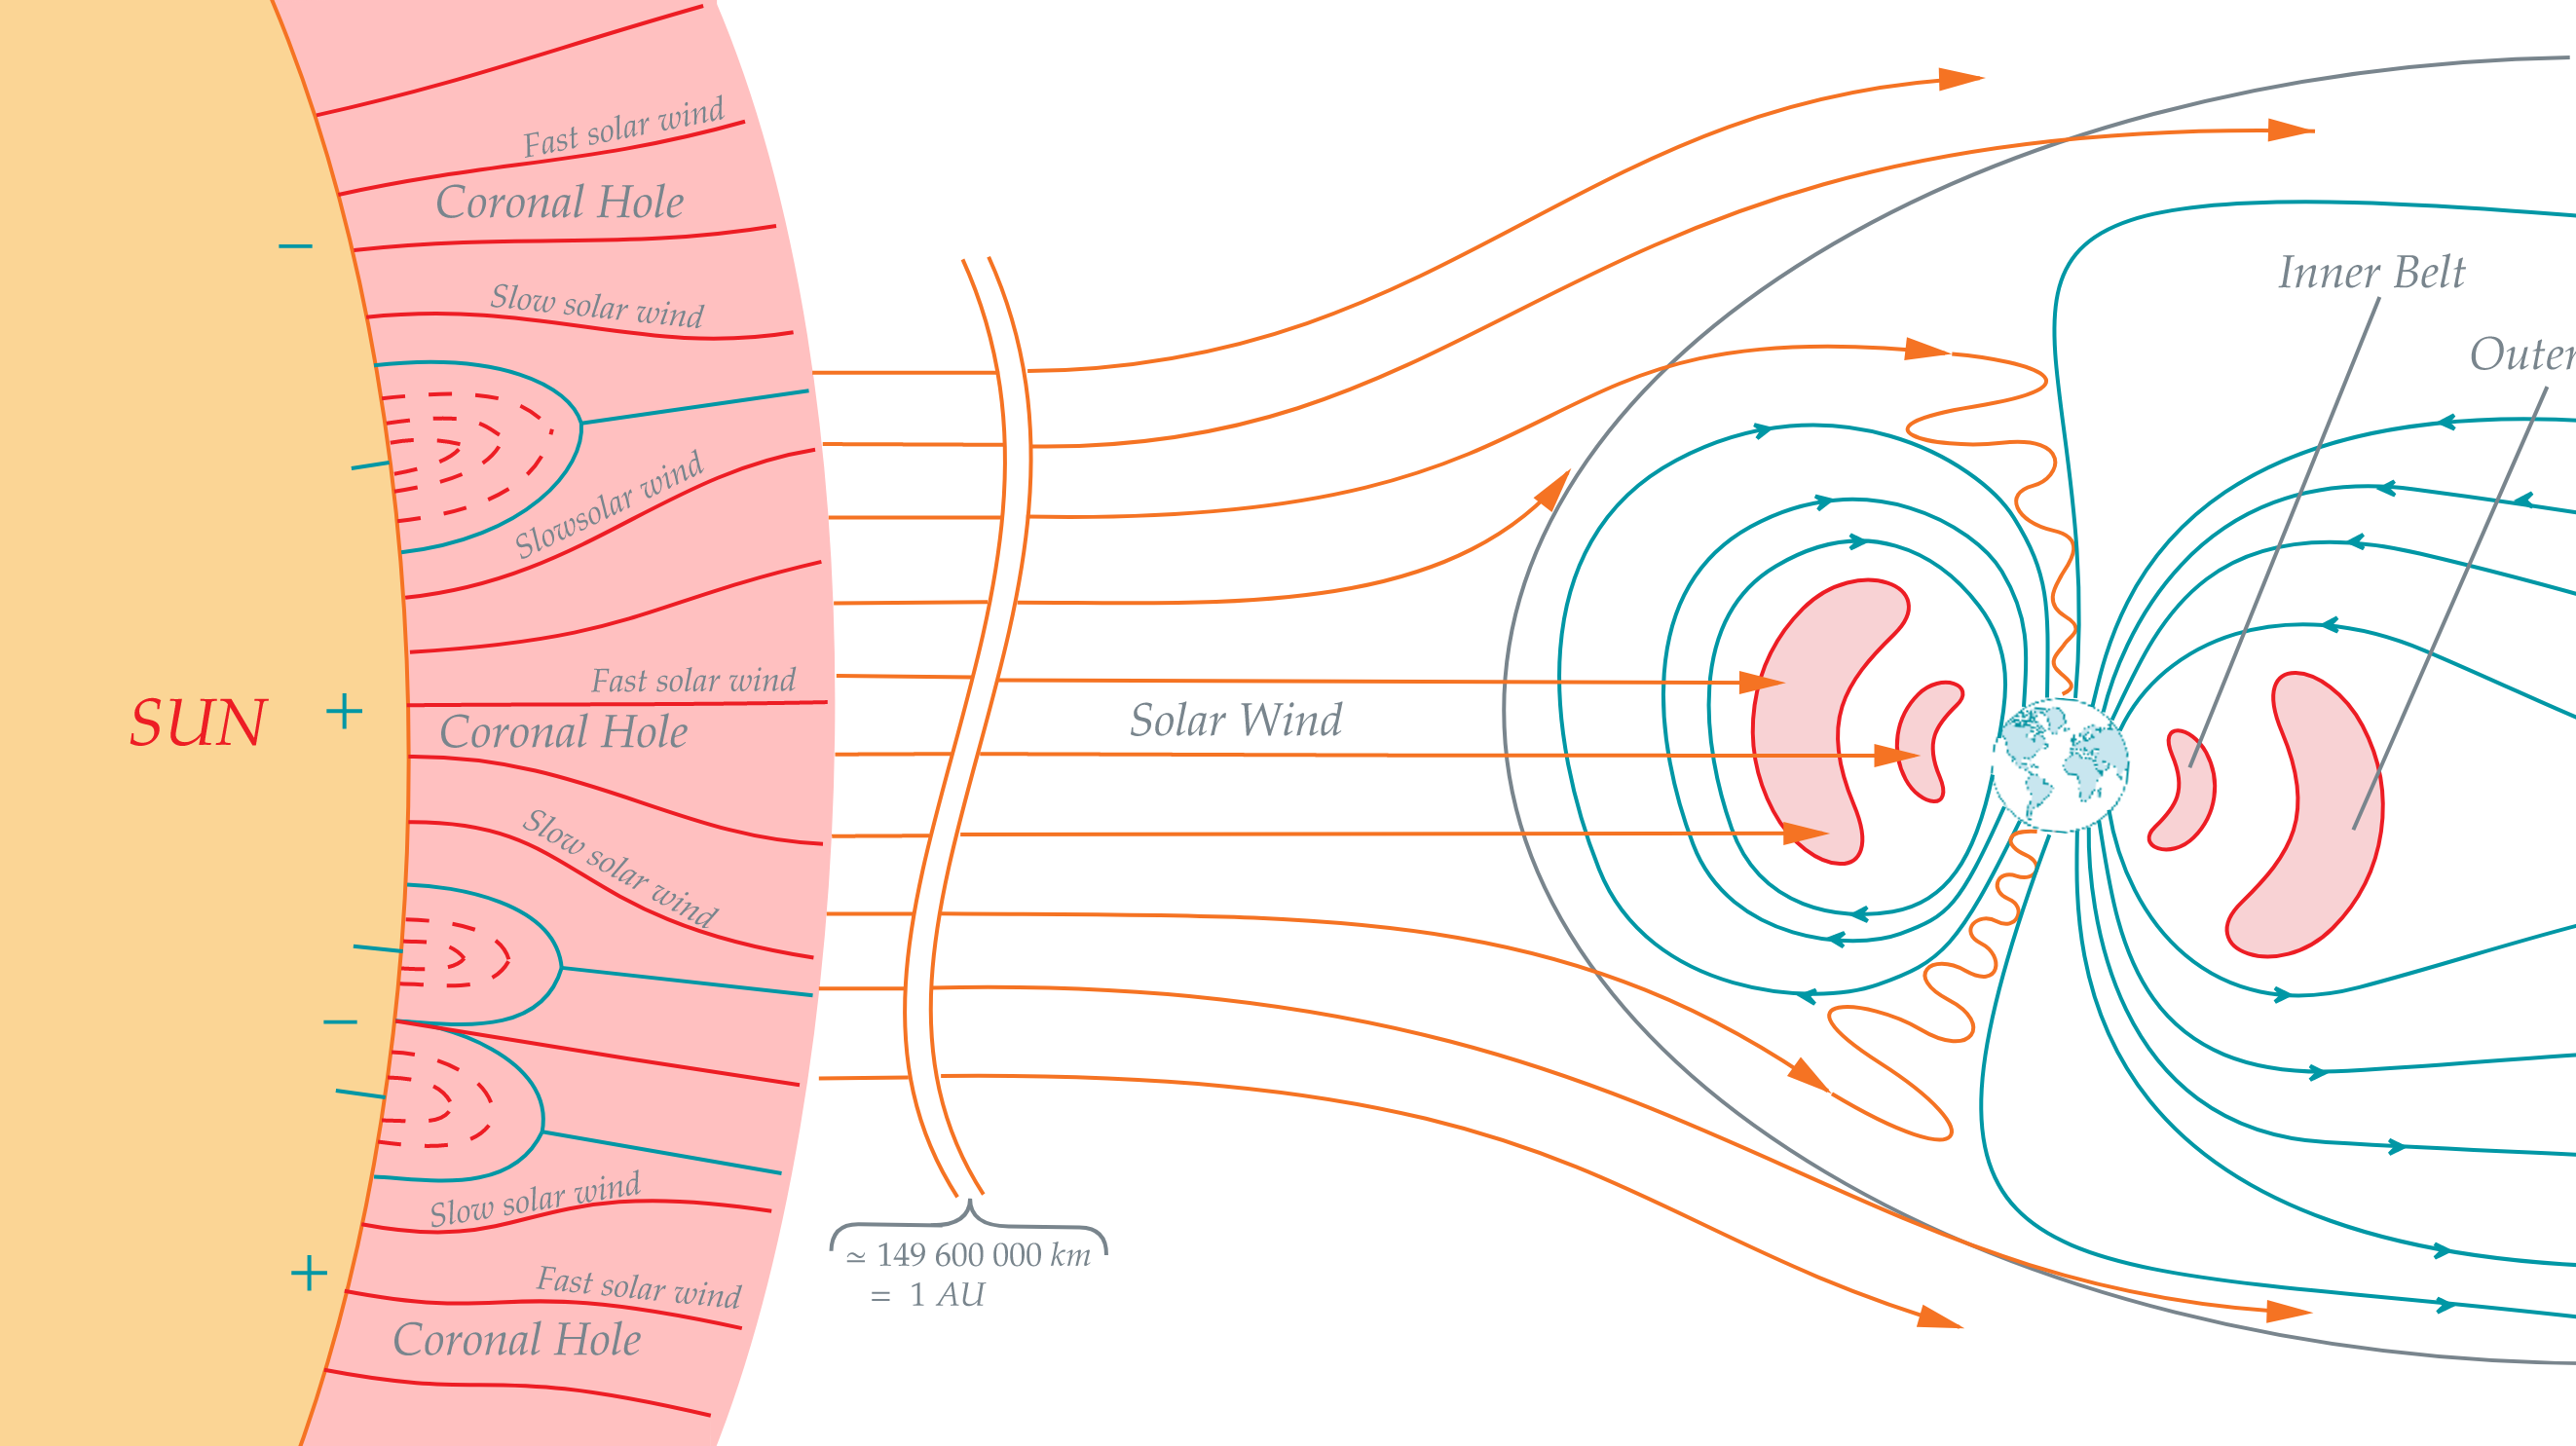
\includegraphics[width=\textwidth,center]{./images/Magnetosfera_e_raggi_solari_coronalHole.png}
					\caption{The figure shows the variation of the Earth's magnetic field due to the solar wind. The Van Allen Belts are also highlighted in light red on either side of the Earth. The Corona of the sun show how magnetic field changes particle ejection.}
					\label{fig:MagnetosphereVanAllenBelts}
					\end{figure} 
				
					The emitted particles are mainly photons, protons, electrons, alpha particles and a small number of heavy ions, all of which are energized and ejected at about 400-700km/s out of the sun. The ejection is due to the high temperatures (6000K) and the inability of the Sun's gravitational force to hold the particles because it is too weak at that distance from the nucleus. \\
					
					The solar wind at a distance of 1AU from the Sun  ($149\,597\,900\,km$) strikes the Earth with $500\cdot 10^6\,\, particles/(cm^2\,sec)$ at a speed of 300-450$\,\,km/s$, the average kinetic energy of protons is about $1keV$, while for electrons it is $10eV$ \bscite{Venkatesan1985}. Because of the low kinetic energy of the solar wind, it is normally trapped in the Van Allen Belts or deflected by the Earth's magnetic field. But when phenomena such as solar flares, CMEs and prominences occur the energy of the ejected particles is higher and particles with $E\,>\,1GeV$ can be detected on the ground, these energized particles are called Solar Energetic Particles (SEPs) and have energy of $1\,MeV$ to $1\,GeV$.\\
					
					The main problem with SEPs is that over a period of a few hours or days they have a very high flux of up to an excess of $500\,000/(cm^2\,sec)$, so solar activity can create serious problems for space mission electronics.
		
					When the solar wind reaches the Earth, it changes the Earth's magnetosphere as shown in \figref{fig:MagnetosphereVanAllenBelts}. The Earth's magnetic field then deflects much of the solar wind, and the particles that manage to enter the atmosphere (the SEPs and GCRs) collide with hydrogen and oxygen to form a cascade of particles that make up the secondary cosmic rays. \\
					
					As they descend into the atmosphere, Secondary Cosmic Rays continue to collide with nuclei in the air, until they arrive attenuated on earth as Terrestrial Cosmic Rays. The same thing happens to GCRs that normally have higher energies and flux.
				}% end Solar Cosmic Rays
			
				\paragraph{Manufacture and Package materials Radiations}{
					The materials used to build the die and package have radioactive impurities that release alpha particles due to natural decay to more stable atoms. For example, $^{232}Th$ decays by emitting 6 alpha particles from 4MeV to 8MeV, while $^{238}U$ releases 8 alpha particles with similar energy. For example, in the solder bumps there are some isotopes that create a flux from 7 to 0.002 $alpha\,\,particles/(cm^2\,hr)$ \bscite{RHE}.\\ 
					
					For these reasons, the primary source of alpha particles for a circuit is the package; in fact, any particle emitted by radioactive impurities can be the source of a SEE, since it is ionized and cannot be shielded.\\
					
					Today the limit reached by ULA (Ultra Low Alpha) materials is $\sim 0.001\,\alpha/(cm^2\,hr)$, if each alpha particle generated a SEE we would have about one million FITs, but in reality we have only from 1000 to 100 FITs in common chips since not all alpha particles generate a SEE. This is why in terrestrial applications the main cause of error is due to the isotopes impurities of the package since neutrons are few and rarely create SEE. As the altitude rises, the effects are reversed because the neutrons are increasingly energetic and they cause more SEEs.  
					
				}% end Package Radiations

				\paragraph{Medical Radiation}{
					Radiation in medicine is used in exams (X-rays) and sterilization (X-rays, gamma rays, e-Beams), normally the maximum observable dose in an examination is 20mSv (millisievert) equal to $2\,rad_{Si}$, this dose is normally harmless even for commercial electronics.  
					
					On the other hand for sterilization the radiation is much higher ($\sim\,5\,Mrad$) making it impossible for even military electronics to survive, so normally if you have electronics in a device to be sterilized, you either use other techniques or switch it off in order to reduce the damage. 
					
					In fact the TID depends very much on the electric field, which is absent if the circuit is switched off \bscite{RHE}.  
					
				}% end Medical Radiation
						
				\paragraph{Nuclear Power Plants}{
					In nuclear power plants and industrial environments, there are sources of X-rays, gamma rays, e-beams and neutrons.
					
					TID effects are the main effects on electronics, although in particular applications (such as measuring the temperature of the cooling ponds of nuclear reactors) the electronics are subject to too much radiation ( even for hardened circuits ) and must therefore be replaced periodically to prevent deterioration.
				} % Nuclear Power Plants
			
				\paragraph{Nuclear Weapon}{
					The effects of a nuclear explosion depend on the location of detonation and on the power of the bomb. Many nuclear bomb experiments are carried out in the air, the Hiroshima bomb itself detonated at an altitude of 580m, and some explosions have occurred in water and soil. 
					
					For an air blasting, immediately after the explosion is formed a fireball filled with strong radiation and temperatures of $10\,000^\circ C$, it expands over a 1km radius for Megaton. The fireball in turn creates a pressure wave that reaches 5 to 10 psi and speeds up to $1000 km/h$, reaching a distance of 5-7km for Megaton. Thus about 50\% of the bomb's energy is converted into the explosion, while 3\% becomes thermal energy which heats the explosion site and can explode fuel reserves up to 10km away per Megaton.\\
					
					The initial radiation in the fireball makes up about 5 \% of the bomb's energy and is composed of gamma particles (at the speed of light (c)), X-rays and neutrons (at 15 \% of speed of light with $12.14MeV$). After the initial explosion, 35\% of the energy is converted into Fallout, a residual radiation composed of secondary fission products and neutron-activated products that fall out of the atmosphere for weeks after the explosion \bscite{RHE}.\\
					
					Another very important effect for the circuits is the EMP generated immediately after the explosion, in fact the radioactive emission reacts with the atmosphere, the ionosphere and the magnetic field in three different phases: in the first phase there is a short pulse of a few nanoseconds caused by the hydrogen and oxygen ionized by the Gamma particles, followed immediately by the second phase with a pulse of about 1sec produced by the reflected Gamma rays and by the reactions of the neutrons with the atmospheric nuclei in the air. \\
					
					Finally, the last pulse is formed by the radiation ionizing the upper ionosphere and distorting the magnetic field. This variation in the magnetic field couples with the energy transmission lines, creating strong pulses in the distribution network, which destroys devices and transformers and causes extensive damage \bscite{RHE}.\\
					
					The circuits involved in a nuclear explosion, depending on the distance of the epicentre, may suffer all or some of the above effects.
				}% end Nuclear Weapon
			
			}% end Sources of radiations
		
		
			\subsubsection{Radiation Effects on ICs}{
				As far as \textit{nuclear radiation} and \textit{Cosmic Rays} are concerned, there is a bombardment of the IC with Alpha or Neutron particles, which penetrate the material and release energy in the form of electron-hole pairs. Depending on the energy of the colliding particle and the sensitivity of the circuit the generated charges can cause a bit flip or soft error. \\
				
				The sensitivity of the circuit is expressed in \textit{Critical Charge}, which is the charge required in a circuit to create a bit flip. The energy of the particle is referred to as \textit{Stopping Power} that is the energy lost per unit length by the trace left in the material by an Alpha Particle, it is measured in $eV/\mu m$.
				
				The\textit{ interaction mechanism of Alpha particles and Neutrons} is different: Alpha particles directly generate electron-hole pairs (this is why the SP refers to Alpha particles), while Neutrons interact with the atoms of the material in an elastic or anaelastic mode. \\
				
				The most dangerous interaction is the anaelastic one, because Neutrons decay into other particles (Alphas, Pions, Muons, Neutrons, Deuterons and Tritons) which in turn generate charges in the material. Normally the particles generated by Neutrons have a higher Stopping Power than Alpha particles and lower penetration ranges. Because of this, Neutrons generate a high charge for a short time (hence high current pulses) while Alpha particles create a charge streak that lasts longer (creating low but prolonged currents)\bscite{Mukherjee2008}.\\
				
				In the case of Neutrons impact, an example of how the Soft Error Rate can be modelled is the following \bscite{ImpactCMOSNeutron}:
				\begin{equation} \label{SER_Neutron}
				SER_{circuit}\;\;= \;\;K\;\phi_{Neutrons}\;A\;e^{\frac{Q_{crit}}{Q_{coll}}}
				\end{equation}
				Where K is a constant depending on the technological processes, $\phi_{Neutrons}$ is the Neutron flux, A is the area of the IC involved, $Q_{crit}$ is the Critical Charge and $Q_{coll}\;=\;collected\;\;charge\,/\,generated\;\;charge$ (the ratio between the collected and generated charge per unit volume). From the formula \figref{SER_Neutron} it can be seen that as the critical charge decreases, the SER of the circuit increases; there is also a linear dependence with the area and the neutron flux.\\
				
				The effects of radiation on the components concern the various types of problems that generate the physical mechanisms explained above. They can be divided into Cumulative Effects and Single Event Effects, the former is caused by continuous exposure to energized particles and the latter is due to the effects of a single particle collision. The effects of each group are described in detail below.
			
				\paragraph{Cumulative Effects CEs}{
					The cumulative effects of radiation cause progressive degradation of the components, in fact the exposure to primary and secondary cosmic rays generates long-term changes in the ICs, these defects lead initially to component degradation and subsequently to faults.
					
					There are three main cumulative effects:
					\begin{itemize}
						\item  \textbf{Surface Charging Damage Effect} (SCDE) :The charges generated by an energy particle can accumulate inside an insulating material in the IC and if the phenomenon continues, they generate electrostatic discharge (ESD). Normally an ESD create noise, bit-flip, latch-up and false signals \bscite{Yang2017}. The more energized the particles, the more frequent this phenomenon occur.
						
						\item \textbf{Total Ionizing Dose} (TID) : In this case the charges created by the particles are deposited in the bulk or other active parts of the IC such as the gate, these charges lead to degradation of the $V_{th}$, Leakage currents and timing skew. The TID is expressed in Gray (Gy) or rad ($100rad=1Gy$) where $1Gy=1j/kg$, normally in space or avionics missions the typical received TID varies from 1 to 100 $krad_{Si}$ \bscite{ECSS2016}, it usually depends on the orbit, shielding and many other factors that vary the incident radiation on the chip.
						
						\item \textbf{Total Non Ionizing Dose} (TNID) : TNID is that portion of particles that do not create electron-hole pairs but instead directly apply a momentum to the semiconductor material. This energy applied to the lattice crystal is transformed into defects and variations from the crystal shape. In turn the degradation of the crystal structure leads to degradation in the parameters of the component, especially in optoelectronic systems \bscite{ECSS2016}. 
						
					\end{itemize}
					
					These effects occur mainly in the avionics and space environment where the particles are more energetic and their flux is orders of magnitude higher than on earth.
					
				}% enb Cumulative Effects CEs
				\paragraph{Single Event Effects}{
					Single Event Effects are due to the charges deposited by the particles, SEEs can be either temporary or permanent effects. They are divided into Destructive SEEs that generate permanent damage in the circuit and Non Destructive SEEs that cause damage reparable with fault tolerance mechanisms or by a system reboot.\\
					
					There are four principal Non Destructive SEEs:
					\begin{itemize}
						\item \textbf{Single Event Transient} (SET) : This event is a temporary voltage change in a node of an integrated circuit, it is caused by a single particle releasing charges as it penetrates the material. SEUs, SEFIs and other spurious phenomena can be generated by a SET.
						
						\item \textbf{Single Event Upset} (SEU) : The SEU is an event that corresponds to a bit-flip of a memory element: a latch, a Flip-Flop or e.g. the cell of a flash . If the corrupted memory is not used or is corrected  by ECC, it is called a Silent SEU. The probability of a SEU depends very much on the critical circuit charge, the supply voltages and the size of the transistors.
						
						\item \textbf{Multiple Cell/Bit Upset} (MCU, MBU) :Both MCU and MBU are caused by the corruption of the value of two or more adjacent cells by a particle. The difference is that MCU occurs between cells of different words while MBU occurs between cells of the same word. This difference is substantial because in a memory with ECC that can correct only one bit, MCUs are correct while MBUs can't be correct since they cause two or more errors in the same word.
						
						These phenomena are increasing in new generations of memories since the proximity between cells continues to grow \bscite{ECSS2016}.
						
						\item \textbf{Single Event Failure Interrupt} (SEFI) : This event is defined as the soft error that causes a reset or stall of a circuit component or the whole system \bscite{ECSS2016}. It is usually caused by corruption of control memory or program memory, by communications disturbances and internal control signals \bscite{Investigation_SEFI_2015}.
						
						There are also three different types of SEFI, some can be repaired with a software reset, other need power cycling due to a stall and some need partial reprogramming due to corrupted program data.
						
					\end{itemize}
					
					
					
					
					Instead destructive SEEs are more technology dependent and they is divided in \bscite{ECSS2016}:
					\begin{itemize}
						\item \textbf{Single Event Latchup} (SEL) : This event occur when the parasitic PNPN or NPNP thyristor of the CMOS structures are turned on. When this happens and the power supply is on, the component can be destroyed by thermal effects. This mechanism don't exists in SOI systems because there are no parasitic thyristor.
						
						\item \textbf{Single Event Snap Back} (SESB) : This event occurs when NPN or PNP parasitic bipolar structures in CMOS circuits are activated. These parasitic transistors can self-sustain a current that can be destructive. SOI technology also suffers from this effect because parasitic transistors are present in these systems. 
						
						\item \textbf{Single Event Hard Error} (ESHE also Stuck-bit) : The ESHE or Stuck-bit is a permanent or intermittent modification of a memory element. This applies to both memories and digital circuits. It differs from an ESHE because it is permanent, in the sense that that memory cell can no longer be used by the system after the event.
						
						\item \textbf{Single Event Gate/Dielectric Rupture} (SEGR, SEDR) : This event indicates the breakdown of a gate oxide or dielectric by a single particle. SEGR and SEDR are dangerous events because they have much faster dynamics than SEL, SESB and SEHE. For this reason, there is no protective circuitry against these events.  In any case they are rarer events and occur mainly in the space environment where there are very energetic particles. 
					\end{itemize} 
					
				} % end Single Event Effects
			}% end Radiation Effects on ICs
		}% end External Factors - Radiation
			
		\newpage
		\subsection{Soft Errors}{
			% Article & books
			% 1.9 of: 2008 Architecture design for soft errors 
			% 1.1 of : (Book) Fault tolerant Systems
			% Avoiding core's DUE & SDC via acoustic wave detectors and tailored error containment and recovery
			% Reducing DUE-FIT of caches by exploiting acoustic wave detectors for error recovery
			%A Hierarchical Fault Detection Method for Aerospace Embedded Software
			% new/Design and Evaluation of Hybrid Fault-Detection Systems
			All the possible transient errors analyzed in the previous chapters are Soft Errors, these errors remain in the memory elements (e.g. flip-flops, latch) only until a new value is written.
			
			
			When fault detection and correction systems are applied to a system, two categories of errors are created at system level:
			\begin{itemize}
				\item \textbf{SDC (Silent Data Corruption) :} a faulty bit without detection is read and it modifies the final result of the program.
				\item \textbf{DUE (Data Unrecoverable Error) :} when a faulty bit with only error detection is read. At this point if the bit changes the final result is True DUE, otherwise it is a False DUE.   
			\end{itemize}
			SDC errors are dangerous because they occur on bits for which errors cannot be detected or corrected, these errors can lead to a system crash and must be transformed into DUE errors by error detection or corrected. \\
			
			The advantage of converting SDC errors into DUE is that DUE are detectable  and they lead the system in fail-stop mode. In fact once a DUE is detected, the system stops and evaluates how to continue execution. At the operating system level, if the error is inside a process we can kill only that one and we talk about process-killer DUE, otherwise we say that DUE is system-killer because the OS has to restart the machine to avoid the propagation of the error.\\
			
			DUE and SDC errors have different effects on dependability; DUE causes Availability penalties because the system has to recover, while SDC lowers Reliability, Safety and Availability because it can crash the system. 
			For these reasons normally there is a budget of TDC and DUE expressed in FIT, for example  228FIT of SDC (500 years of MTTF) and 57000FIT of DUE (2 years of MTTF) by specification.   
			\paragraph{Time Vulnerability Factor (TVF)}{
				The TVF is the fraction of time in which the circuit is vulnerable to errors. It is calculated using the window of vulnerability (WOV), which is the time within the clock period in which the circuit can be subject to SEE, for example in edge-triggered flip-flops the WOV is equal to half the clock because only in that interval the FF change state if it is struck by a particle (only in the high/low phase is the data sampled and held). The TVF is therefore the ratio between the vulnerability window and the clock period, so for an edge-triggered FF the TVF is equal to 50\%. 
				
				Actually, the calculation of the TVF is more complicated because the propagation delay of the circuit has to be taken into account, assuming in fact a period of 1ns and an average combinatorial delay of 700ps, in this case the TVF will be lower than 50\% since some faults injected in the first 500ns can be masked by the logic delay.
			}
				
			
		}% end Fault classification
		\newpage
		%\subsection{Masking}{
			% Article & books
			% Chapter 3 on AVF: (book) Fault Tolerant Computer Architecture
			% 2014 hybrid fault Tolerant Technique to detect transient Fault ...
			
			
		%}% end Masking
	
		%\subsection{General Hardening strategy for IC}{
			% Article & books
			% Chapter 2,3,4,5 of : (book) Fault tolerant Systems
			% Chapter 2: Fault‐Tolerance Techniques for Spacecraft Control Computers
		%}% end General Hardening strategy for 

		
	}% end Dependability of Integrated Circuits
	\section{Hardening techniques for digital circuit architectures}{
		% Article & books
		%	
		Hardening techniques are used to improve the dependability of a system and they can be applied at each design layer as described in section \ref{ElectronicSystemParts}. We now focus on digital circuits architecture hardening technique that  are used in order to increase the Safe Failure Fraction (SFF) and so increase the SIL of the architecture.
		
		\subsection{Spatial redundancy}{
			% Article & books
			%	
		    Spatial redundancy consist in use N parallel system which output are voted, this structure decrease the failure rate of the overall system. Indeed when a cosmic ray collide with one of the parallel system and cause an error the other system continue to work properly. Since the probability of a multiple strike is lower than particle flux we have a reduction in cosmic ray sensibility. \\
		   
		    Another advantage in the use of redundant system is the increase of MTTF. Indeed using N parallel system each with the same $\lambda=\frac{1}{MTTF}$ we have this new MTTF \bscite{FTS2021}:
		    \begin{equation}
		         MTTF_{Overall\,\,\,\,System} = \sum_{k=1}^{N} \dfrac{1}{\lambda k}
		    \end{equation} 
		    This formula highlight the increase in MTTF due to the use of parallel systems, this means that it is able to protect also from permanent fault. Anyway not all spatial redundancy techniques increase the MTTF, this normally is not a problem since in safety-critical application since the system is replaced much earlier then its MTTF. \\
		    
		    All Spatial Redundancy techniques can be used both in low level architecture for example an FSM and in high level architecture such as cores. The first use is called \textit{Fine Grain Redundancy} while the second one is called \textit{Coarse Grain Redundancy}.  
		   
		    We have shown that general parallel system is able to protect mainly by transient fault and secondarily by permanent fault. In the next paragraph we analyze the main kind of spatial redundancy techniques from architectural point of view. Any of this system is based on the general M-of-N system that is composed by N modules and needs at least M of them to work properly.
		    
		    \subsubsection{Double Modular Redundancy (DMR)}{
		        An example of Double Modular Redundancy is shown in figure \ref{fig:DMR1}, the basic idea is the use of two identical blocks. When there aren't faults OUT1 and OUT2 are equal and so the output will be OUT1, instead when the two replicas have different outputs is selected the Safe Output and is asserted an Error Detection. 
		        
		        The assertions of the Error Detection signals are normally handled at software level, here should exist a routine that enable recovery of the previous state and a new execution of the faulty step.
		        
		        \begin{figure}[H]
        			\centering
        			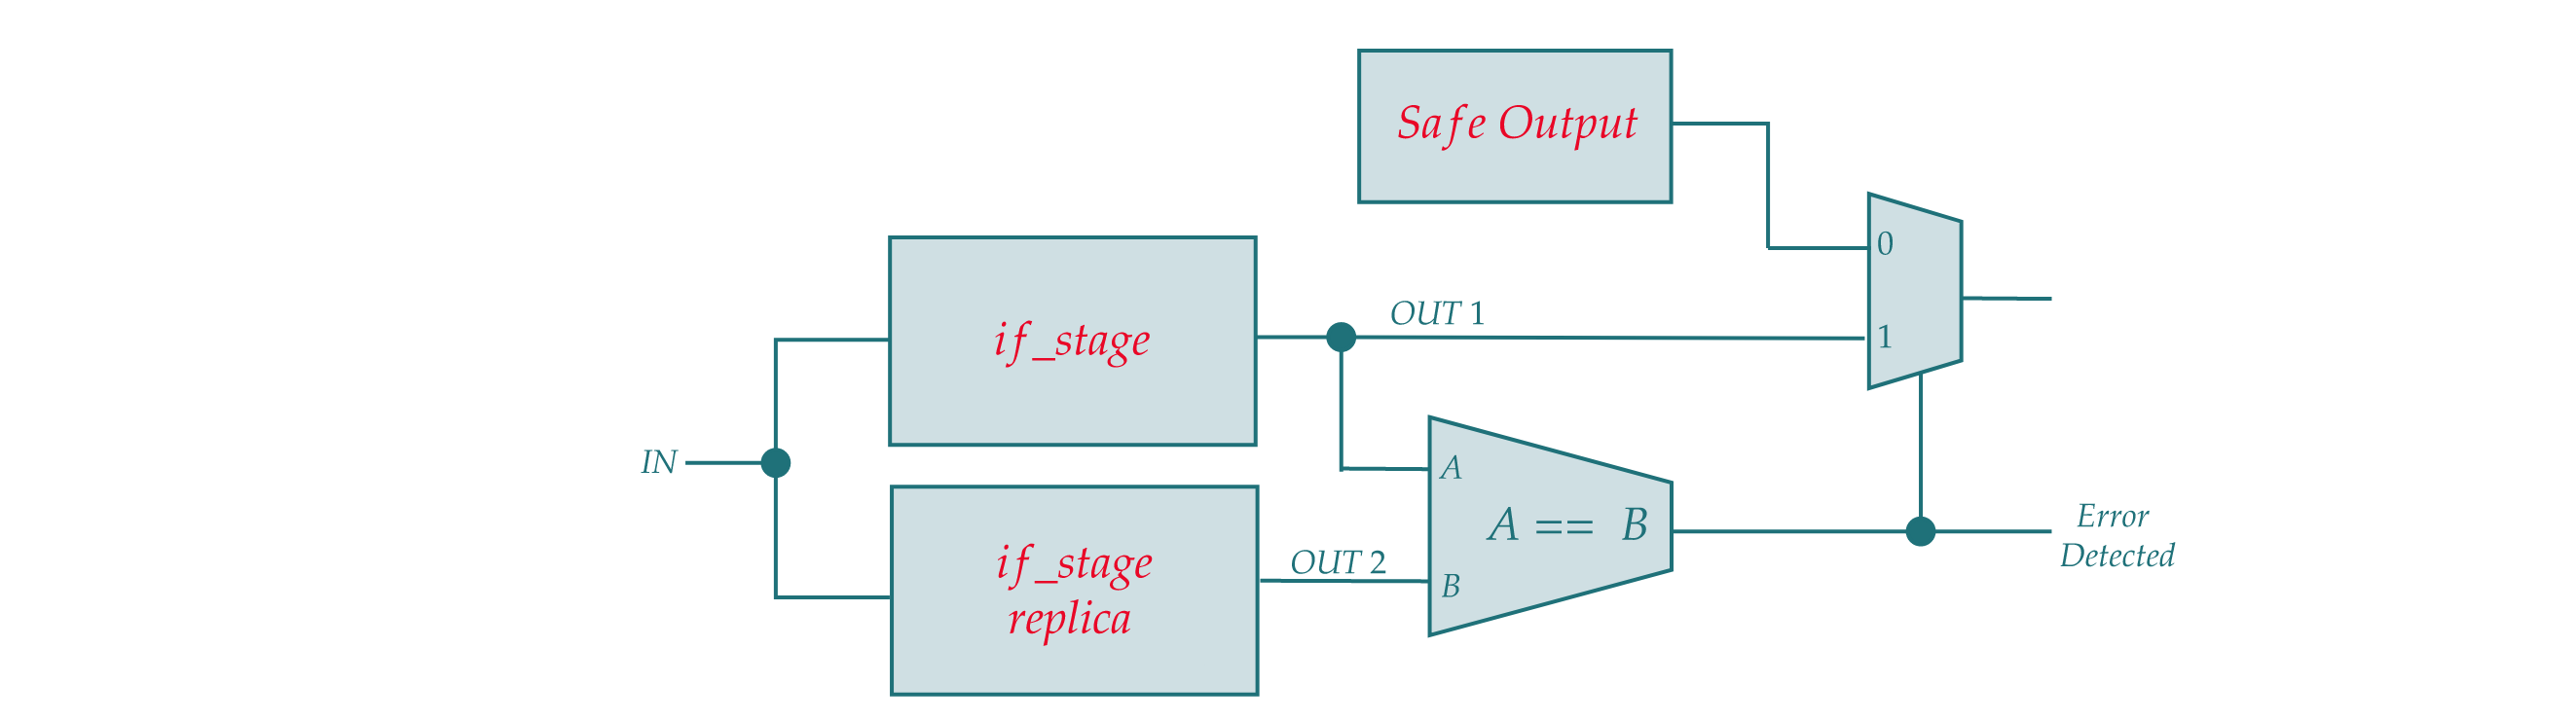
\includegraphics[scale=0.2,center]{./images/DMR1.png}
        			\caption{Example of DMR using an if stage of a core}
        			\label{fig:DMR1}
        		\end{figure} 
        		
        		DMR add time penalty when a fault occur because normally the execution should be repeated to obtain the correct output, indeed DMR is only able to detect a fault. 
        		
        		In figure \ref{fig:DMR1} we use the if\_stage of a processor but DMR can be used at whatever level, e.g. at core level using two identical core in parallel.
		    }
		    \subsubsection{Triple Modular Redundancy (TMR)}{
		        In figure \ref{fig:TMR1} there is an example of TMR using the if stage of a core, as you can see are used three replicas of the same stage working in parallel, the outputs from the stages are voted to find correct value using majority voter.
		        
		        \begin{figure}[H]
        			\centering
        			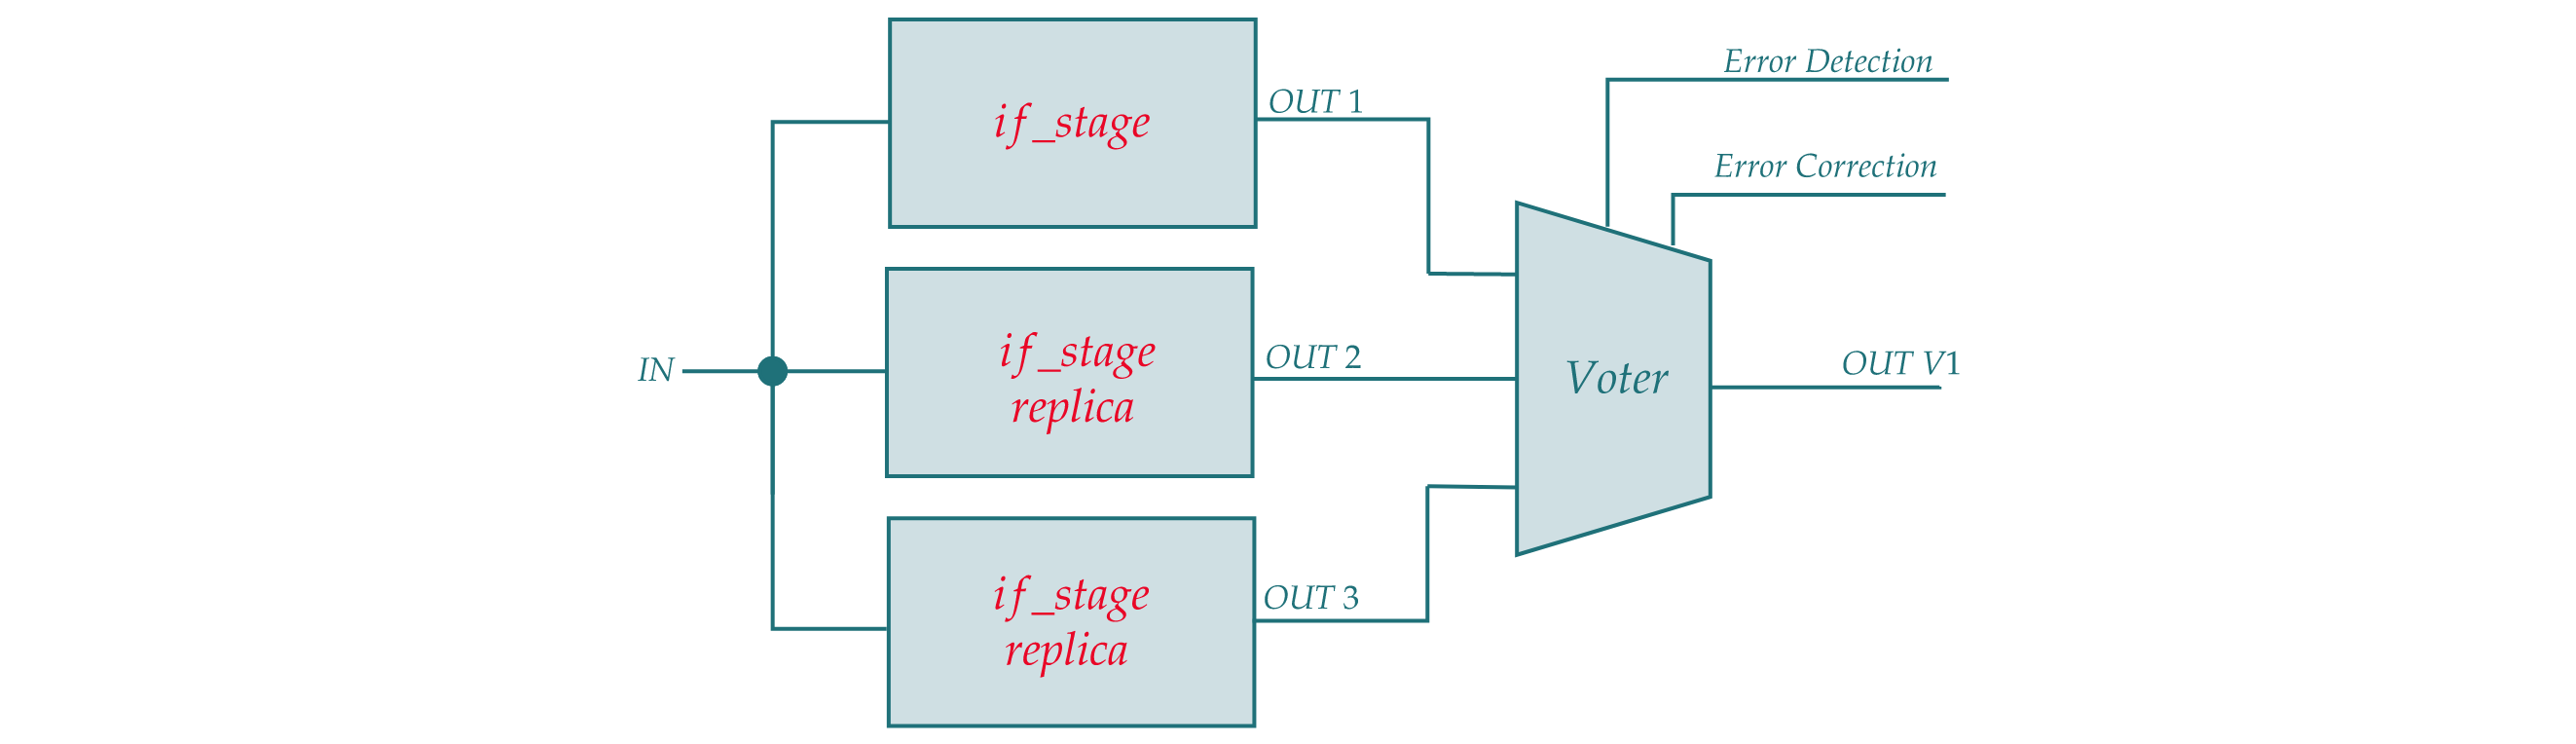
\includegraphics[scale=0.2,center]{./images/TMR1.png}
        			\caption{Example of TMR using an if stage of a core}
        			\label{fig:TMR1}
        		\end{figure} 
        	
        		This resilient structure is able to detect and correct only one fault, when two error occur in two replicas at the same time this structure isn't able to correct the faults but only to detect it.
        		These are some possible cases of faults:
        		\begin{itemize}
        		    \item \textbf{One error in one replica:} Assume that the fault is in the first replica and so OUT1 is wrong, the voter sees $OUT2=OUT3\neq OUT1$ and so it asserts $OUTV1 = (OUT2=OUT2)$. At the same time is asserted \textit{Error Detected} and \textit{Error Corrected} signals. So in this case the error is detected and corrected.
        		    \item \textbf{Two parallel errors in different replicas:} In this case $OUT1\neq OUT2 \neq OUT3$ and so the voter is not able to detect and correct the output, anyway it asserted \textit{Error Detected} and negates \textit{Error Corrected} signal, in this way high level software or architecture sees that an error occurs. Normally these types of errors are rare in terrestrial environments, since particle flux is low, anyway in the case there is already a permanent error in one replica a SEE would be able to stress such an error. 
        		    \item \textbf{One error in majority voter:} In this case the output will be wrong due to voter errors, this raises questions about voter contribution in the final Safe Failure Fraction. Normally voter is smaller respect to the stage area and so SEEs are low in absolute number, anyway when we use fine grain redundancy we should consider the voter contribution.
        		\end{itemize}
        		
        		The Reliability of a TMR system can be calculated using this formula \bscite{FTS2021}:
        		\begin{equation}
        		    \label{eq:R_TMR}
        		     R_{TMR}(t) = R_{voter}(t)\left( 3 R^2(t) - 2R^3(t) \right)
        		\end{equation} 
        		Where $R_{voter}(t)$ is the reliability of the voter and $R(t)$ is the reliability of the stages ( each stage have the same reliability). As you can see in \ref{fig:3Dplot_R_TMR} the reliability of the voter is important such as stage reliability, as we already mentioned this difference in reliability is assured by the area and complexity difference. 
    		    
    		    \begin{figure}[H]
        			\centering
        			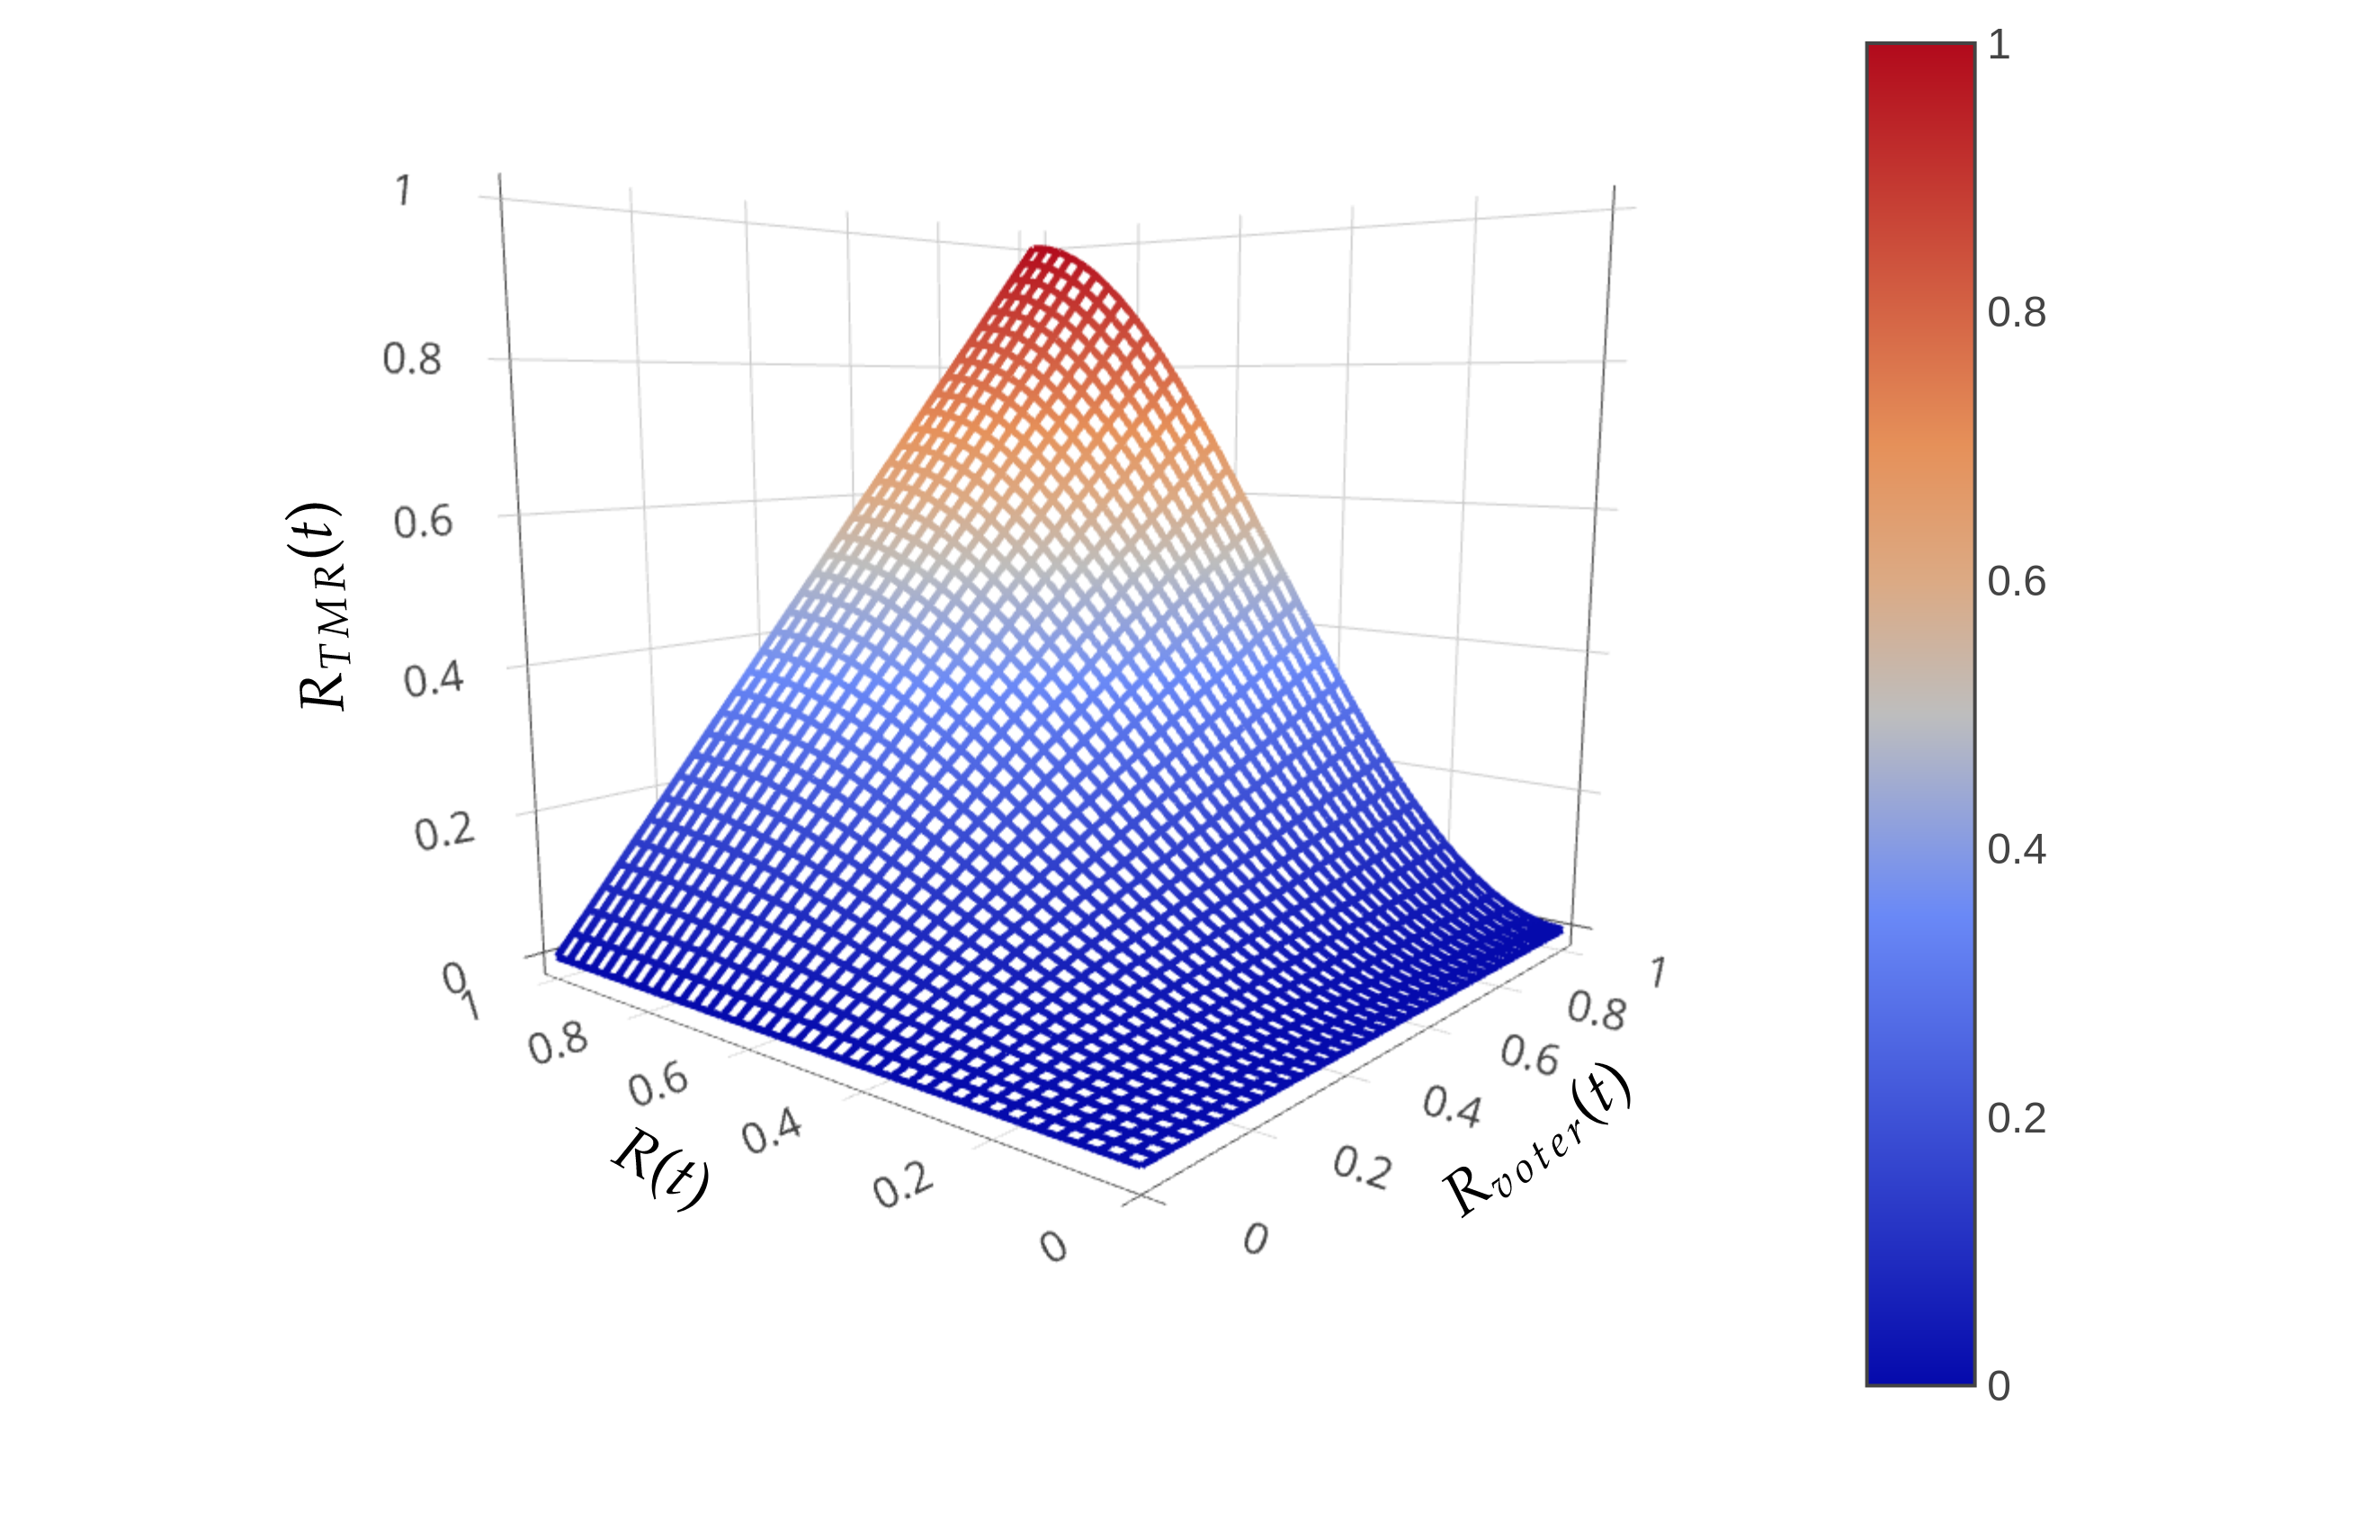
\includegraphics[scale=0.15,center]{./images/TMR_reliability.png}
        			\caption{Plotting of equation \ref{eq:R_TMR}}
        			\label{fig:3Dplot_R_TMR}
        		\end{figure}
        		
        		Now integrating equation \ref{eq:R_TMR} between 0 and $\infty$ we obtain the MTTF \bscite{FTS2021} (we consider $R_{voter}$ about 1):
        		\begin{equation}
        		    MTTF_{TMR} = \frac{5}{6 \lambda} < MTTF_{simplex} = \frac{1}{\lambda}
        		\end{equation}
        		
        		The $MTTF_{TMR}$ is lower then $MTTF$ of simplex system, this is due to the fact that is enough for a stage to break to cause an error. However the MTTF difference is very small, we should also consider that in safety critical application is usually more important the reliability respect to the MTTF since the system is replaced far before R(t) < 0.5 \bscite{FTS2021}.
        		Usually the real MTTF and the Reliability are higher then calculated since we should take into account fault compensation and errors that are masked by the system \bscite{FTS2021}.\\
        		
        		We have seen some advantage and limitation of basic TMR, for the large part of the application TMR is a good solution but sometimes we need an higher level of reliability, in these cases are used TMR with voter triplication or diversity redundancy.
        		
        		\paragraph{Voter Triplication}{
        		    At first glance voter triplication seems to be useless, indeed looking at figure  \ref{fig:TMR2} we have three output from the voters, these three output should be newly voted to find the correct output. Anyway voter triplication is used to connect two TMR stages as depicted in figure  \ref{fig:TMR3}, in this case the use of three voter is useful. 
        		    
        		    
        		    Indeed when one of the voter have a fault the error propagates only in the next stage replica, this error is then deleted by the voter at the output of the system. 
        		    It is clear here that the use of triplication is useful in \textit{fine grain} application in which many stage are protected and connected together.
        		    In the architecture of figure \ref{fig:TMR4} an error in the middle voter propagates in all next stages without any possible correction, this case is avoided by voter triplication.
        		    
        		    The main difference between architecture \ref{fig:TMR3} and \ref{fig:TMR4} is the occupied area, in fact if you have a high number of output from each stage the triplication of voter imply an high number of interconnections and area, this reduce the speed of the circuit and increase the power consumption.
        		    
        		    \begin{figure}[H]
            			\centering
            			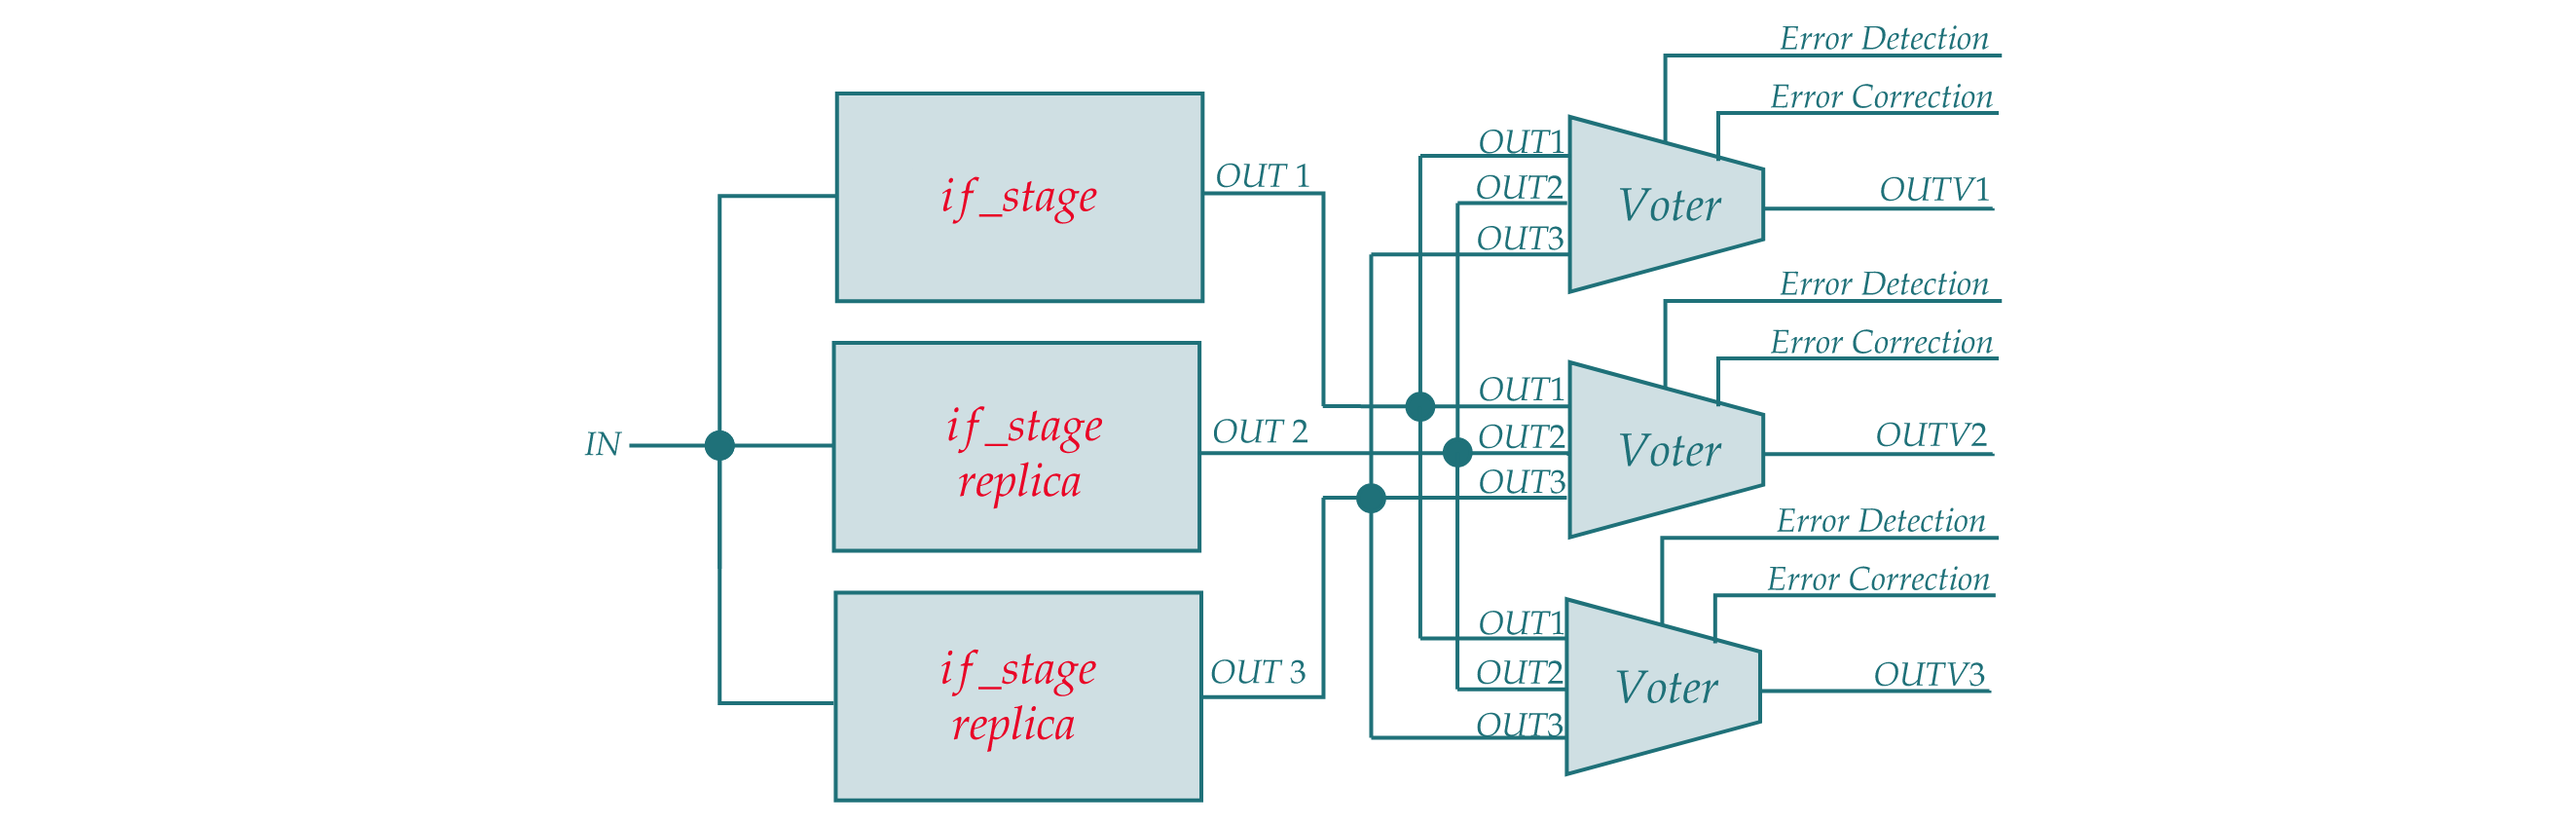
\includegraphics[scale=0.2,center]{./images/TMR_tripleVoter.png}
            			\caption{Example of TMR with voter triplication in only one stage}
            			\label{fig:TMR2}
            		\end{figure}
            		
            		\begin{figure}[H]
            			\centering
            			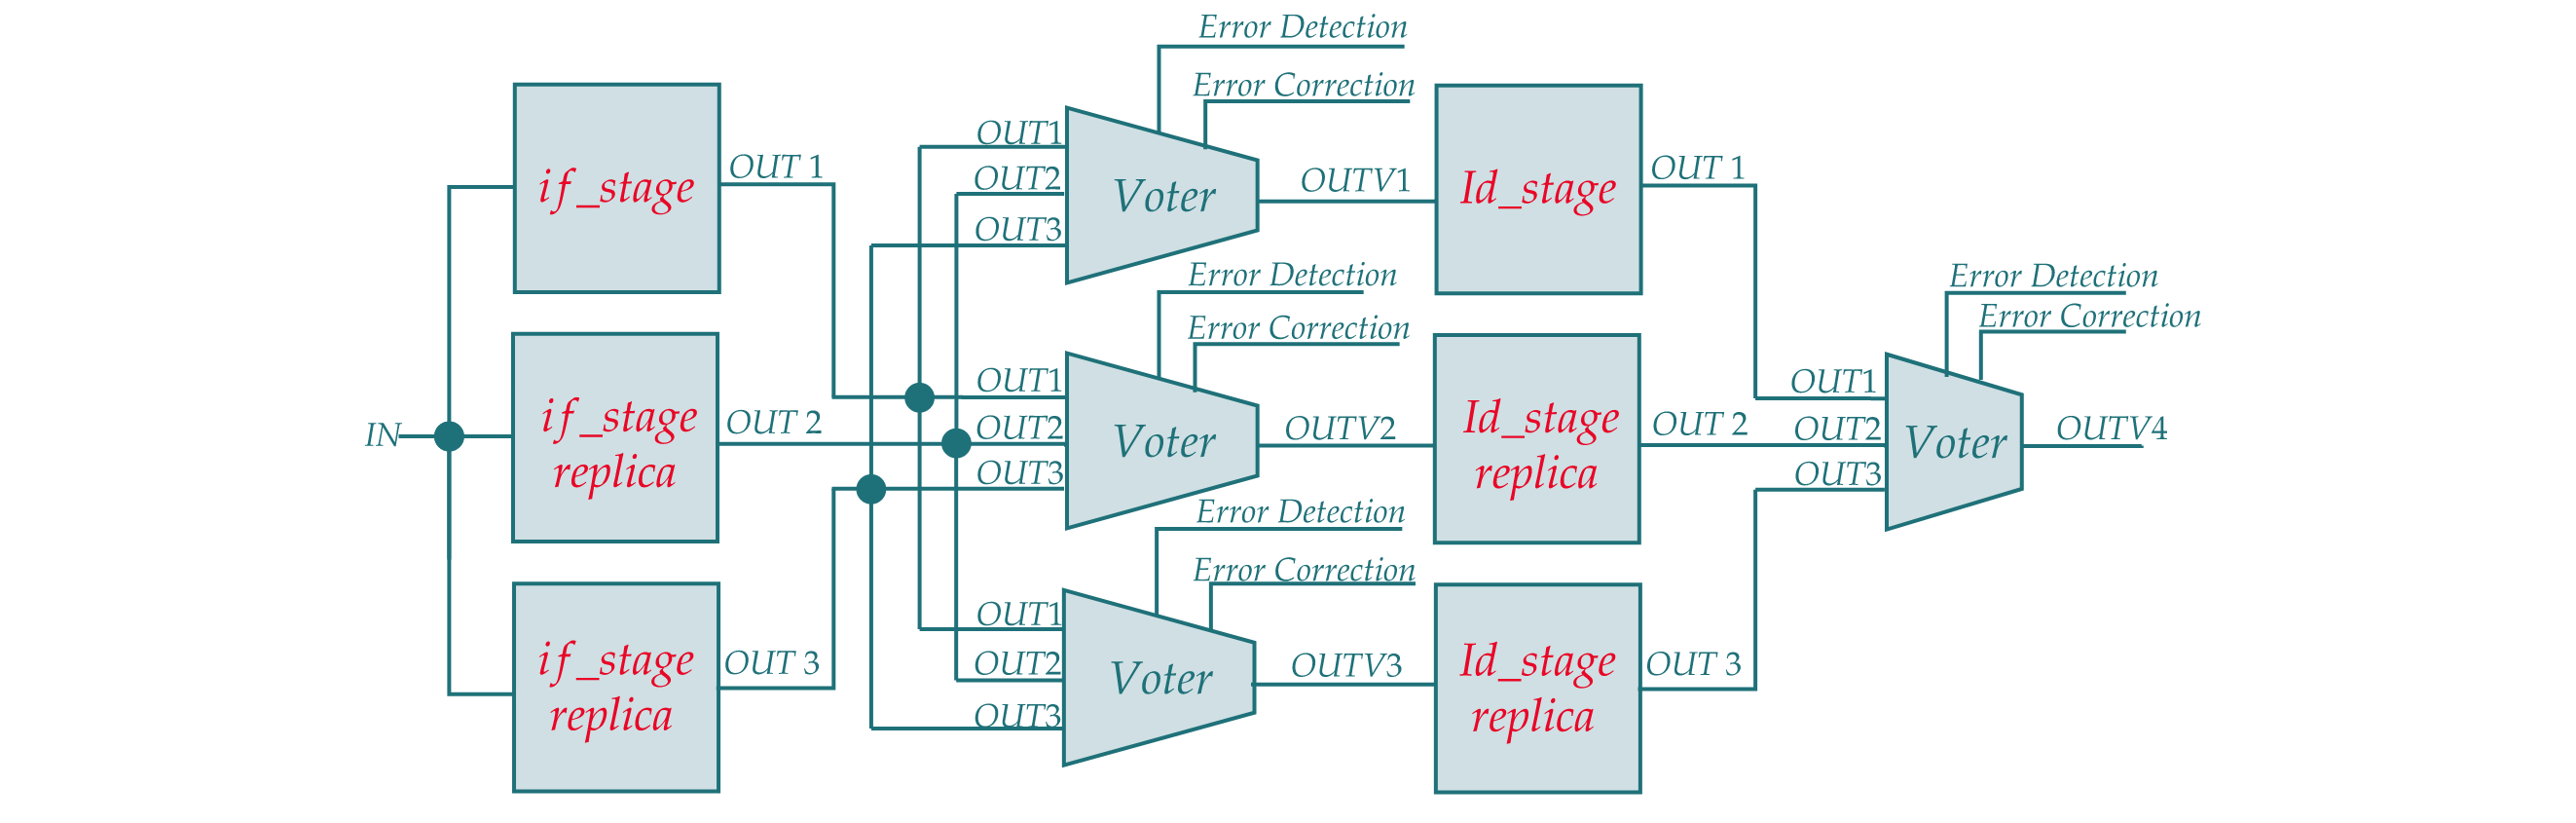
\includegraphics[scale=0.2,center]{./images/TMR_tripleVoter2.png}
            			\caption{Example of TMR with voter triplication used in stages connection}
            			\label{fig:TMR3}
            		\end{figure} 
            		
            		\begin{figure}[H]
            			\centering
            			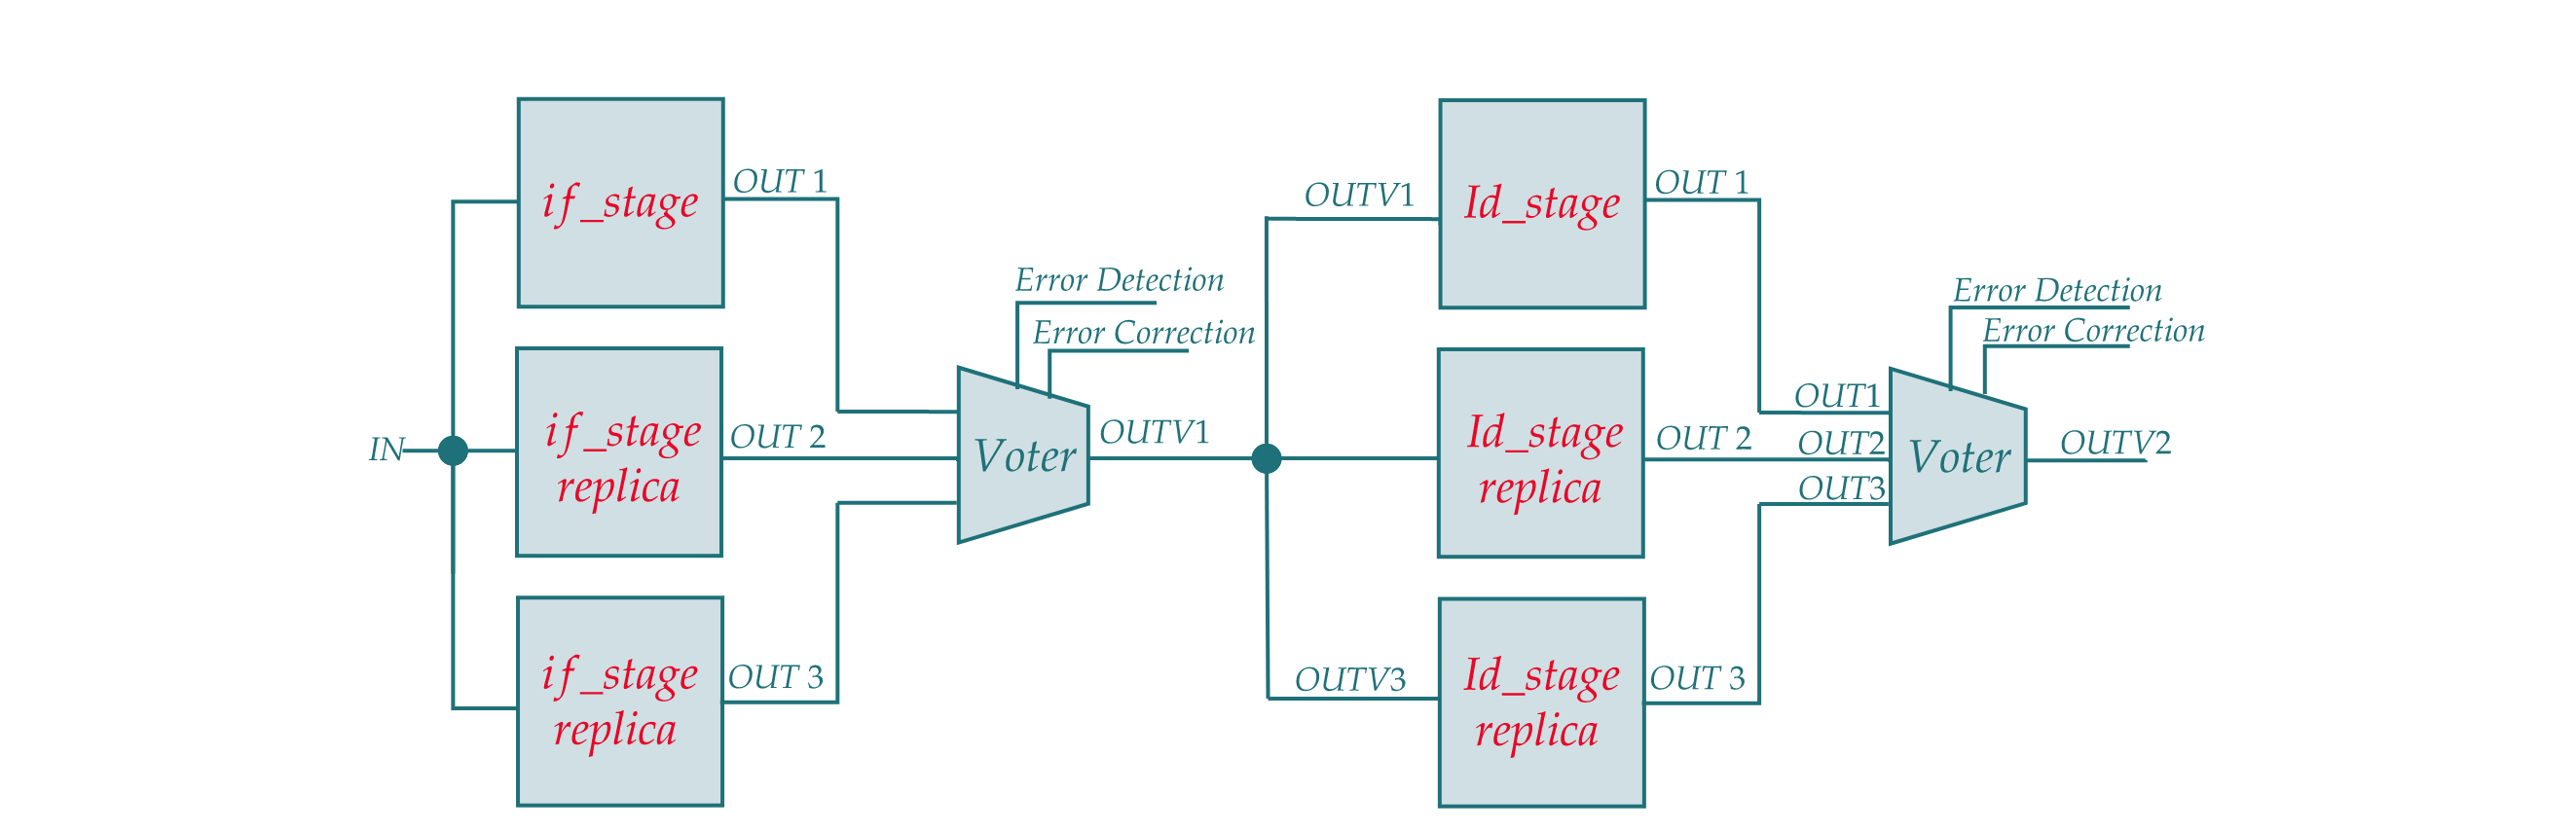
\includegraphics[scale=0.2,center]{./images/TMR_tripleVoter3.png}
            			\caption{Example of TMR used in stages connection, the voter is the weak link of the chain.}
            			\label{fig:TMR4}
            		\end{figure} 
            		
            		Another application of the triple voter is writing into memory, indeed when we have a triplicated memory we could use triple voter, in this way a faulty voter write only a wrong value while other memory are correct. The same argument can be done for memory read, in this case the use of three voter avoid a wrong reading. 
        		}
        		\paragraph{Diversity Redundancy}{
        		    Apart from SEEs and permanent faults there are implementation errors. These types of errors are due to designer implementation mistake but they can be reduced using Design Diversity in redundancy \bscite{DesignDiversity}. An architecture that implements TMR and uses design diversity is shown in figure \ref{fig:TMR5}, as you can see the three parallel stages are designed independently by different teams, this decrease the implementation errors because the probability that two independent teams commit the same mistake is low. \\
        		    
        		    
                	Diversity redundancy is also able to increase the reliability as shown in this reaseach \bscite{Evaluating_the_effectiveness_of_a_diversity_TMR_scheme_under_neutrons}, the paper evaluates the DTMR (Diversity Triple Modular Redundancy) using an FPGA hit by a neutron flux of $3.98*10^4 n/cm^2/s$ (standard deviation of $3.74*10^3 n/cm^2/s$) with an energy of 10MeV for 1268 minutes. 
                	The average number of upsets detected was about one per minute. It was found that the DTMR approach is better than TMR because each redundant block has a different reliability.\\
        		    
        		    This technique increase the cost of the design. Indeed are needed three independent teams that work at the same architecture, this is an extra cost that may be paid for high reliability request, for example a system that should have the maximum SIL. 
            		
            		\begin{figure}[H]
            			\centering
            			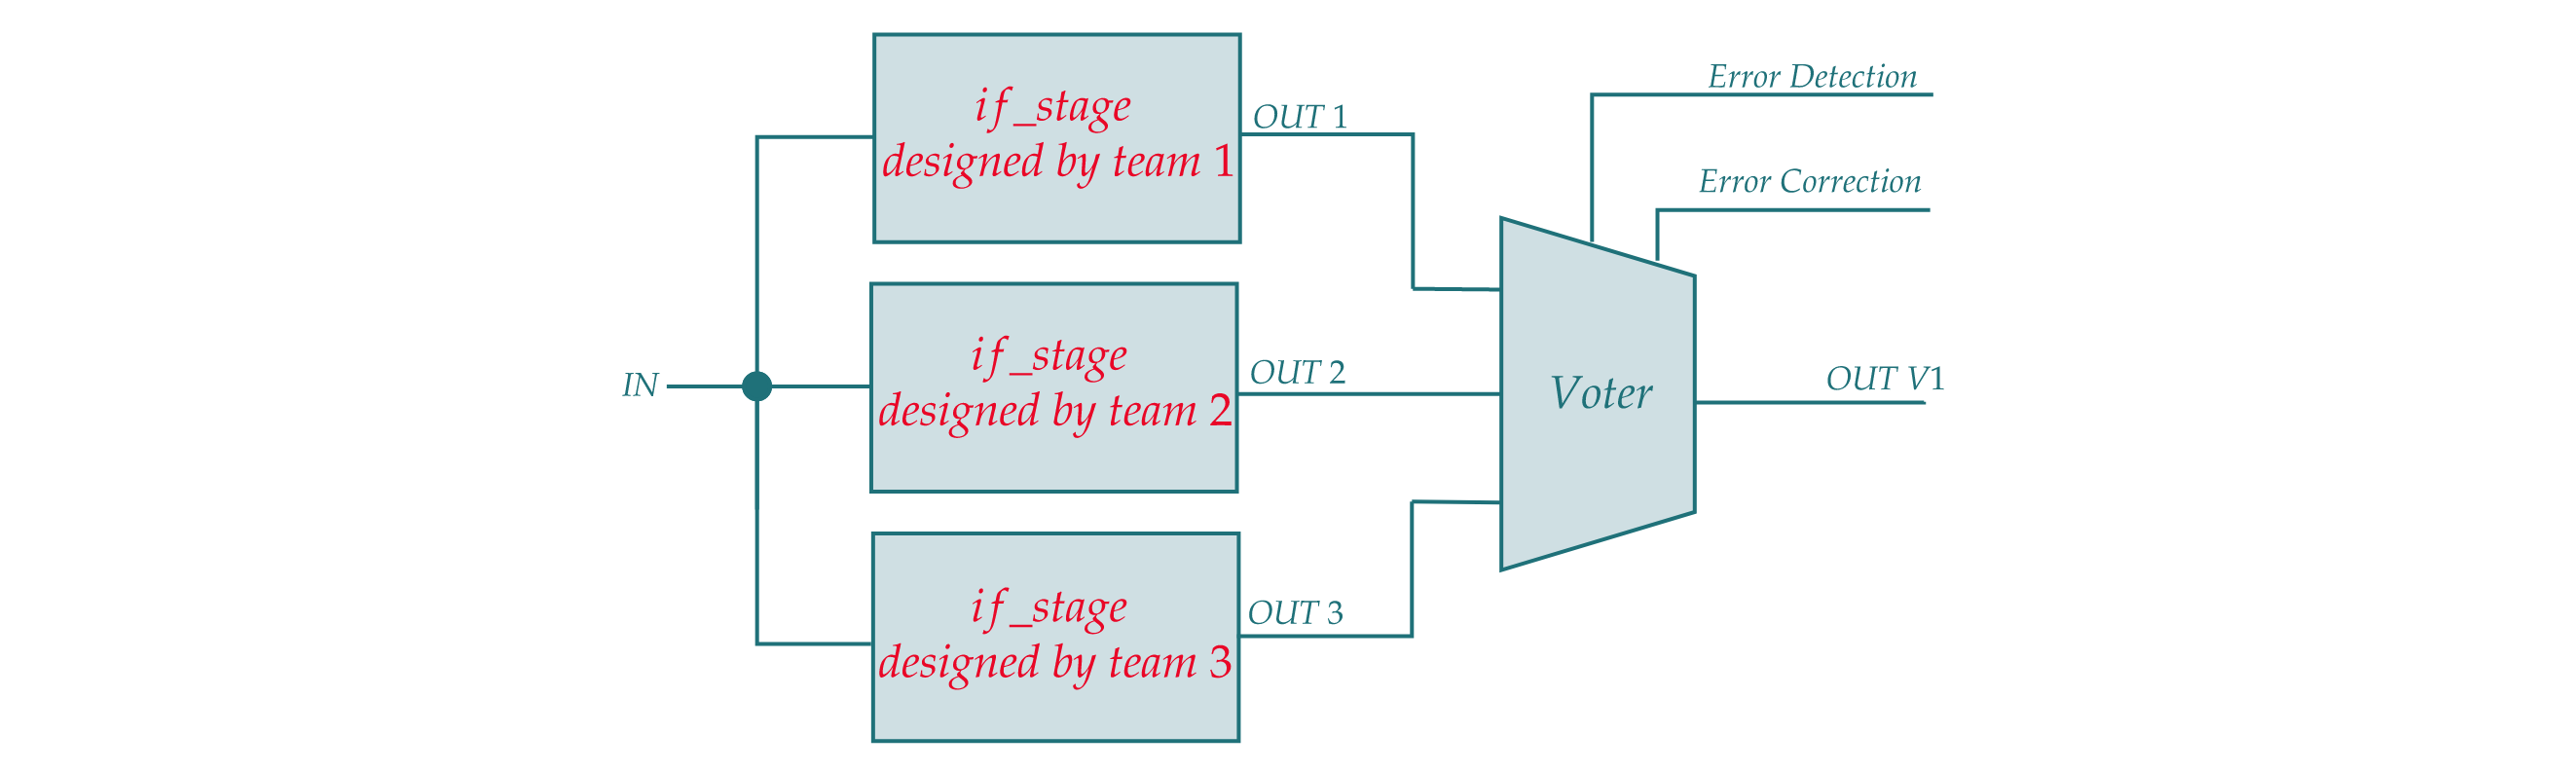
\includegraphics[scale=0.2,center]{./images/TMR_Design_Diversity.png}
            			\caption{Example of design diversity used in conjunction with TMR technique in order to protect an IF stage.}
            			\label{fig:TMR5}
            		\end{figure} 
            		
        		}
		    }
		    \subsubsection{N Modular Redundancy (NMR)}{
		        NMR is a more general set of all techniques that use many parallel block to increase reliability, these system are also called N-of-M where M is the number of redundant system and N is the number of system needed for proper operation. 
		        In order to avoid a deadlock M should be an odd number. As we have seen TMR is a typical NMR system but exist also NMR system with M=5 and upper number, anyway these type of architecture are rarely used due to the high power and area increase, indeed it is known that an increase in the power consumption increase temperature which in turn increase the wearout and probability of SEEs due to particle strike. \\
		        
		        Assuming that all system used in NMR are statistical independent, the general formula of reliability for a NMR system is \bscite{FTS2021}:
		        \begin{equation}
		            \label{eq:R_NMR}
		            R_{N\,\,of\,\,M}(t) = \sum_{i=M}^N \binom{N}{i} R^i(t) [ 1- R(t)]^{N-1}
		        \end{equation}
		        The independence of the parallel blocks is essential and lead to an high reliability, for these reason common mode failure are critical for these system. 
		        Integrating the reliability we find the MTTF of system, as we have seen for TMR the value of MTTF is slightly lower then for simplex architecture and this is also true for all NMR system. 
		        For these reason NMR system are really good in terrestrial application where human is able to maintenance devices and replace end-of-life parts. When we design an architecture for long space mission we can opt for an Hybrid Redundancy.\\
		        
		        Even if for NMR is generally used an odd N number, a 2020 research \cite{Highly-Reliable_Approximate_Quadruple_Modular_Redundancy_with_Approximation-Aware_Voting} investigate the use of Quadruple Modular Redundancy (QMR). The paper proposes an approximate QMR redundancy method where are used three instances that approximate the true result and one that finds the exact one. A vote on the 3 approximate architectures is done first and then the result is voted with the exact architecture. The difference with the other works of approximate redundancy is in the use of approximators equal to each other while in the other works were used all different approximators.  
		    }
		    \subsubsection{Hybrid Redundancy}{
		       As we have seen TMR and NMR increase reliability but slightly decrease the MTTF of the system respect to simplex architecture. This can be a problem in space application where maintenance and replacement are not possible, for these application we can use Hybrid redundancy.
		       As you see in figure \ref{} this technique starts from a NMR architecture adding k spare blocks. During normal operation the N output of the replicas are voted, when a primary block become faulty it is switched off and replaced with a spare block. \\
		       
		       Compare block compares active blocks outputs with correct output and implements a faulty block detector for example using an Alpha Counter for each block. When the Alpha Counter of a block exceeds the critical level, the faulty block is disconnected and replaced with a spare working block.
		       This mechanism implements a self-maintenance system in which end-of-life blocks are replaced, in this way MTTF and reliability of the system are both increased. \\
		       
        		\begin{figure}[H]
        			\centering
        			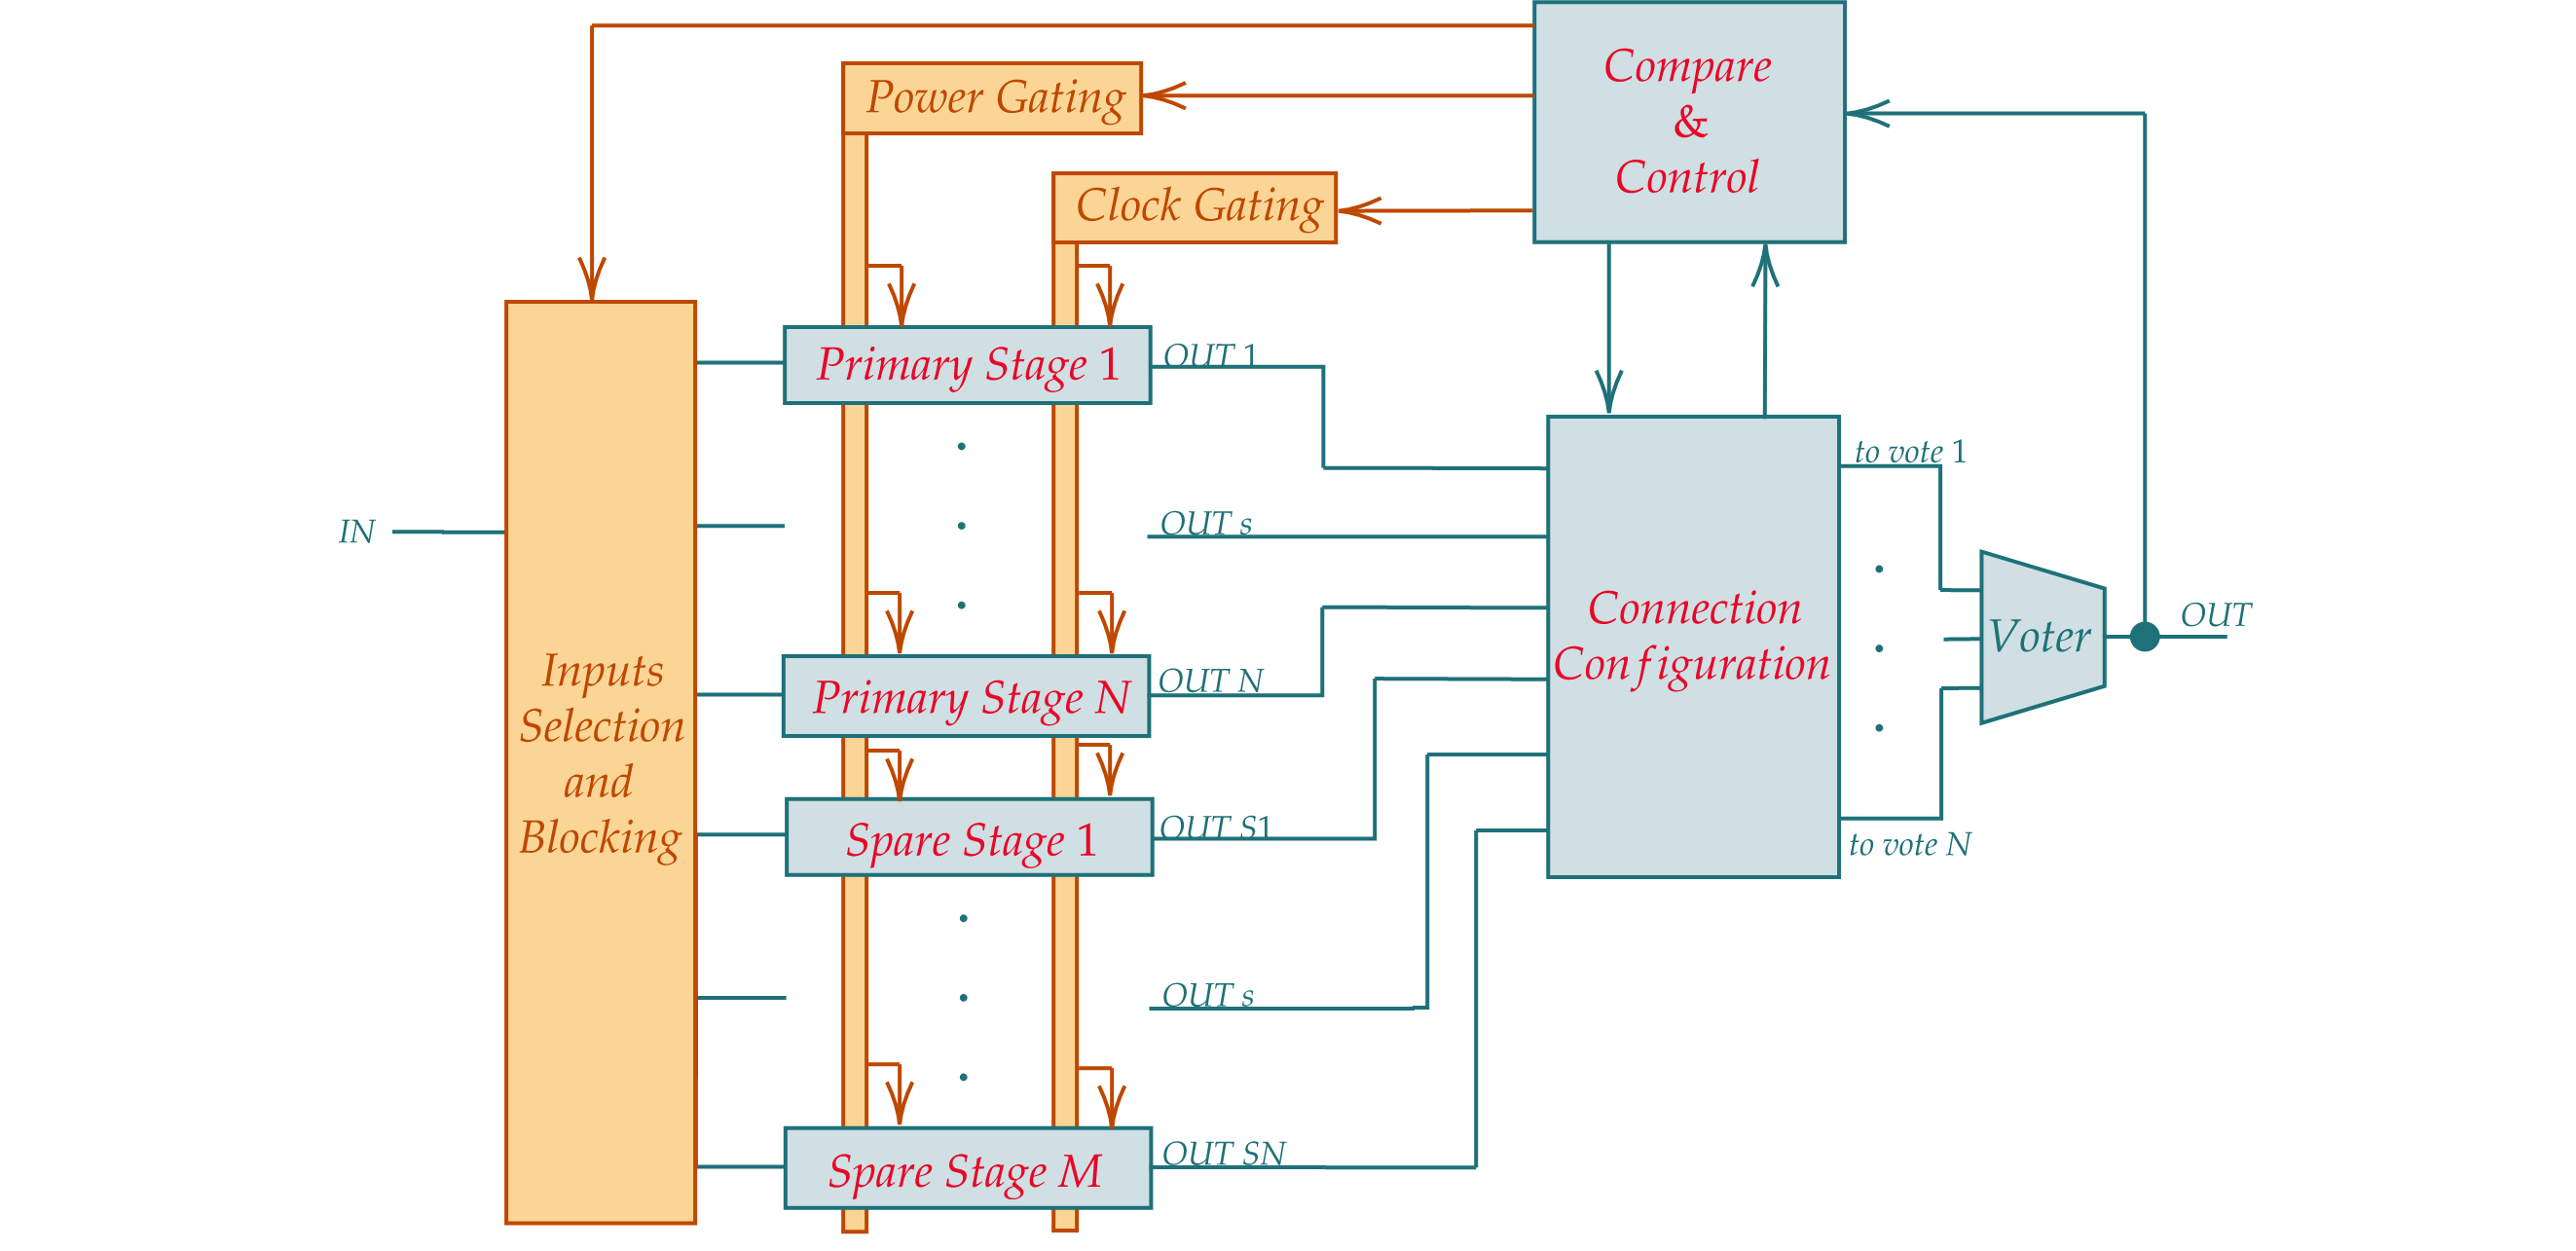
\includegraphics[scale=0.2,center]{./images/HybridRedundancy.png}
        			\caption{Example of generic Hybrid Redundancy with Power gating, clock gating and input selection and blocking.}
        			\label{fig:TMR5}
        		\end{figure} 
		       
		       Spare and primary blocks create a large number of elements to power and control. 
		       The increase of power consumption increase the probability of faults \bscite{Alleviate_TMR_preformance_degradation} and this leads a performance degradation. 
		       To reduce the power consumption designers use clock gating , power gating and input blocking in unused blocks, in this way are reduced useless switches. These methods reduce TID effects since without an electric field the Vth variation is low, this leads to an higher spare block life and an higher system MTTF.\\
		       
		       
		       Clock gating, power gating and input blocking are controlled by compare and control block that should maintain the should also maintain the history of faulty blocks. Problems arise when the system is reset, in these cases there are few methods to recover informations about block status:
		       \begin{itemize}
		           \item \textbf{Common and Status Registers:} These registers are used to store information about hardware and they are readable by software. When a new faulty block is detected the information should saved in one of these register, then a software level routine can move this data in a non volatile memory. When the system is rebooted data from non volatile memory are loaded into CSR and then uploaded into Compare and Control block of each system we have;
		           \item \textbf{Test Vector:} CSR methods is a little complex when we have a high number of Hybrid architecture, it also needs a software procedure. For this reason some designers prefer to avoid CSR methods using a test vector after reboot  \bscite{Combining_FT_and_self_repairing_virtual_TMR}. The system works on this test vector and finds faulty blocks, indeed each Compare and Control blocks correctly configure each hybrid system looking for faulty blocks, at the end of this procedure the the architecture is ready to start in safe mode.
		       \end{itemize}
		    }
		    
		}
		\subsection{Information Redundancy}{
			% Article & books
			% Ecc etc capitolo 8 di soft error in Moder Electronic syste
			% ECC cap 5 di 2008 Architecture design for soft errors 
			% Information redundancy Chapter 3 of : (book) Fault tolerant Systems
			Inside a whatever core memories are used memories to store information, unfortunately also memory experience errors.
		    For these reason there are coding techniques used to detect or/and correct data errors, coding is the most common technique information redundancy. 
		    According to this technique are added some check bits to the original data, this extra bits are stored with the data and are used to verify the correctness of data.\\
		    
		    The information redundancy process is summarized here:
		    \begin{itemize}
		        \item \textbf{Code creation:} The process start when a certain data with A-bits should be written into memory, it is encoded into B-bits codeword. the codeword can be \textit{separable} if check bit and data are not mixed together, so a separable codeword will have A-bits for data and C-bits for check bits where A-bits + C-bits = B-bits;
		        \item \textbf{Data degradation:} The data stored may be modified by SEEs, wear out process and any kinds of possible faults. Statistically the longer the data are not read, the easier they became corrupted due to some faults. This corruption change with memory, technology, temperature, environment etc. and can't be precisely calculated;
		        \item \textbf{Data reading:} When data are read their correctness should be verified. At this step a certain block uses the codeword written in memory in order to detect and/or correct existing faults.
		    \end{itemize}
		    
		    
		}
		\subsection{Temporal Redundancy}{
			% Article & books
			% Chapter 2 and 3 of : (book) Fault tolerant Systems
			The idea of temporal redundancy is to repeat an operation N times and compare results. 
			This decrease the area of a safety architecture but also decrease the performance, as you can see in figure \ref{fig:TemporalRedundancy1} a certain operation is executed three times, the outputs are stored and at the end of computation they are compared to find correct output. 
			This techniques is effective at processors level, where spatial redundancy adds too much overhead, using this techniques can be used only one core plus some external logics.\\
			
			\begin{figure}[H]
    			\centering
    			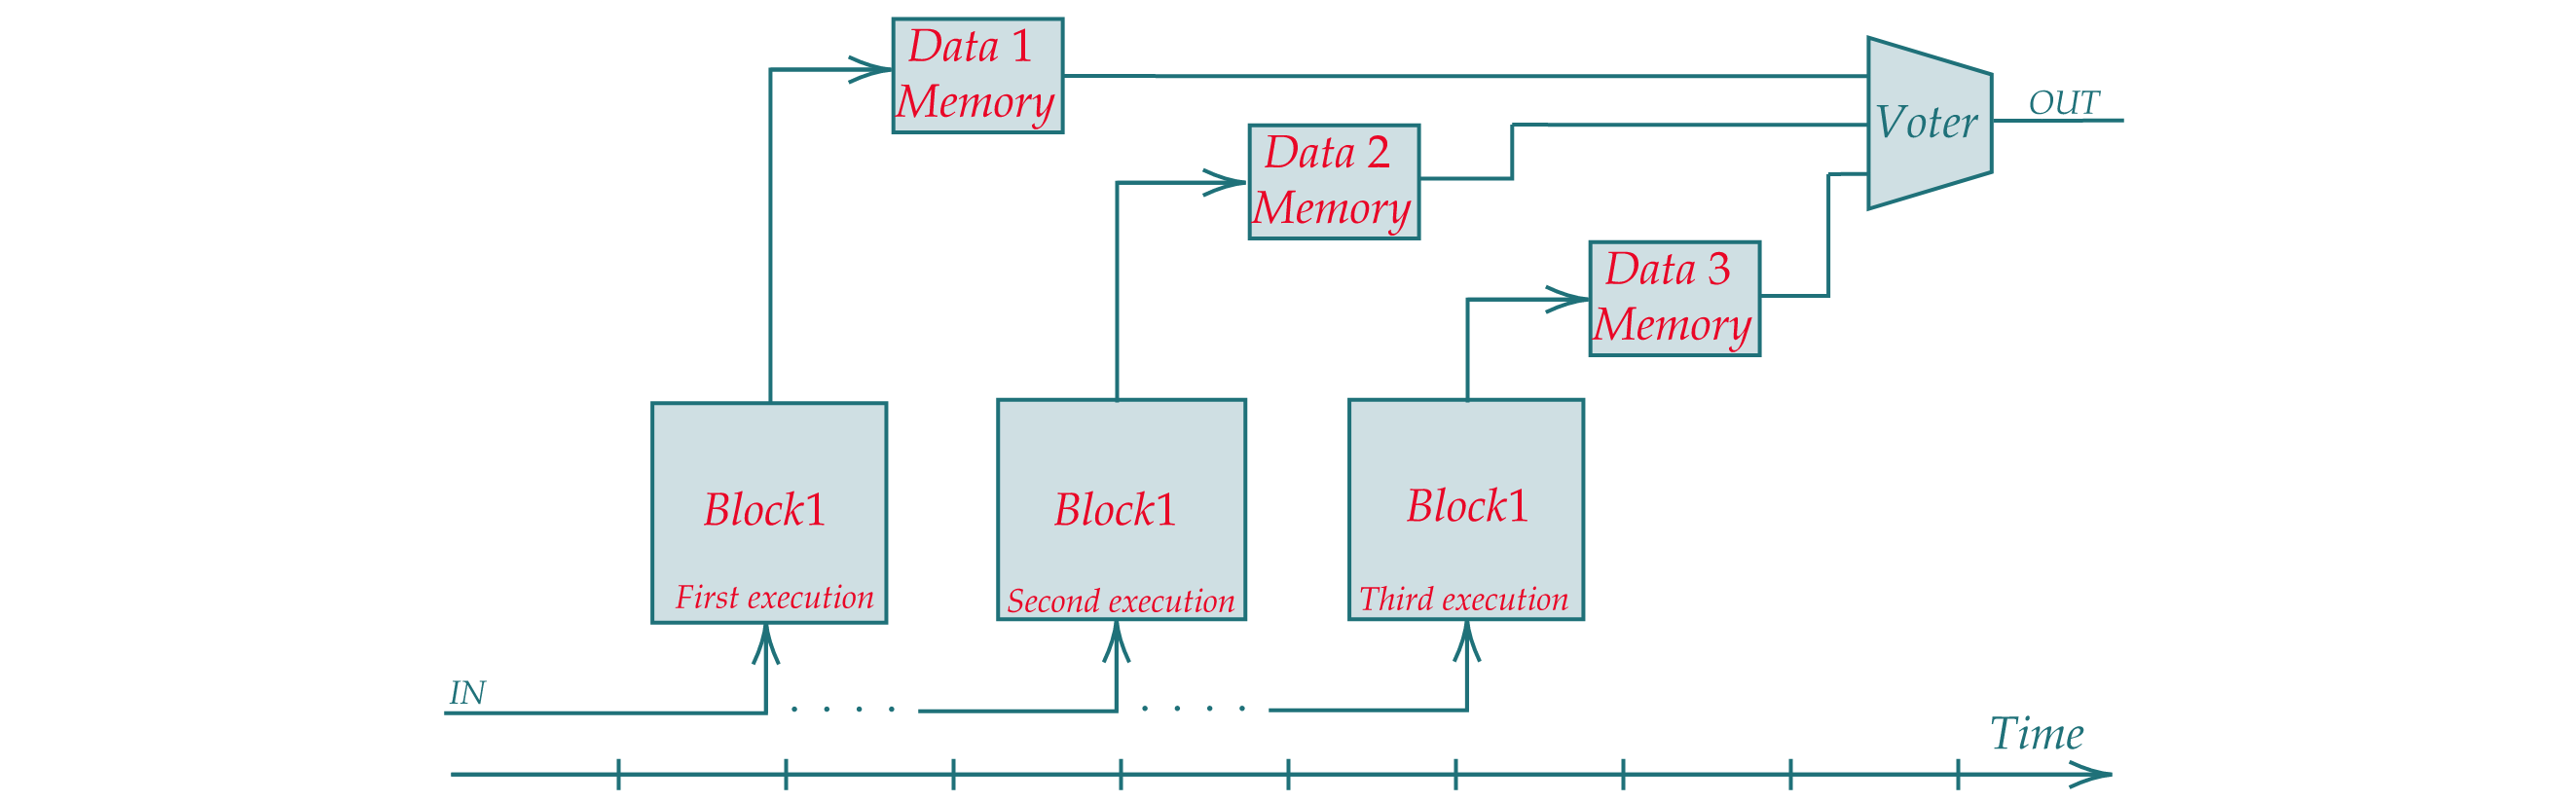
\includegraphics[scale=0.2,center]{./images/TimeRedundancy1.png}
    			\caption{Example of generic Temporal Redundancy.}
    			\label{fig:TemporalRedundancy1}
    		\end{figure} 
    		
    		
			\begin{figure}[H]
    			\centering
    			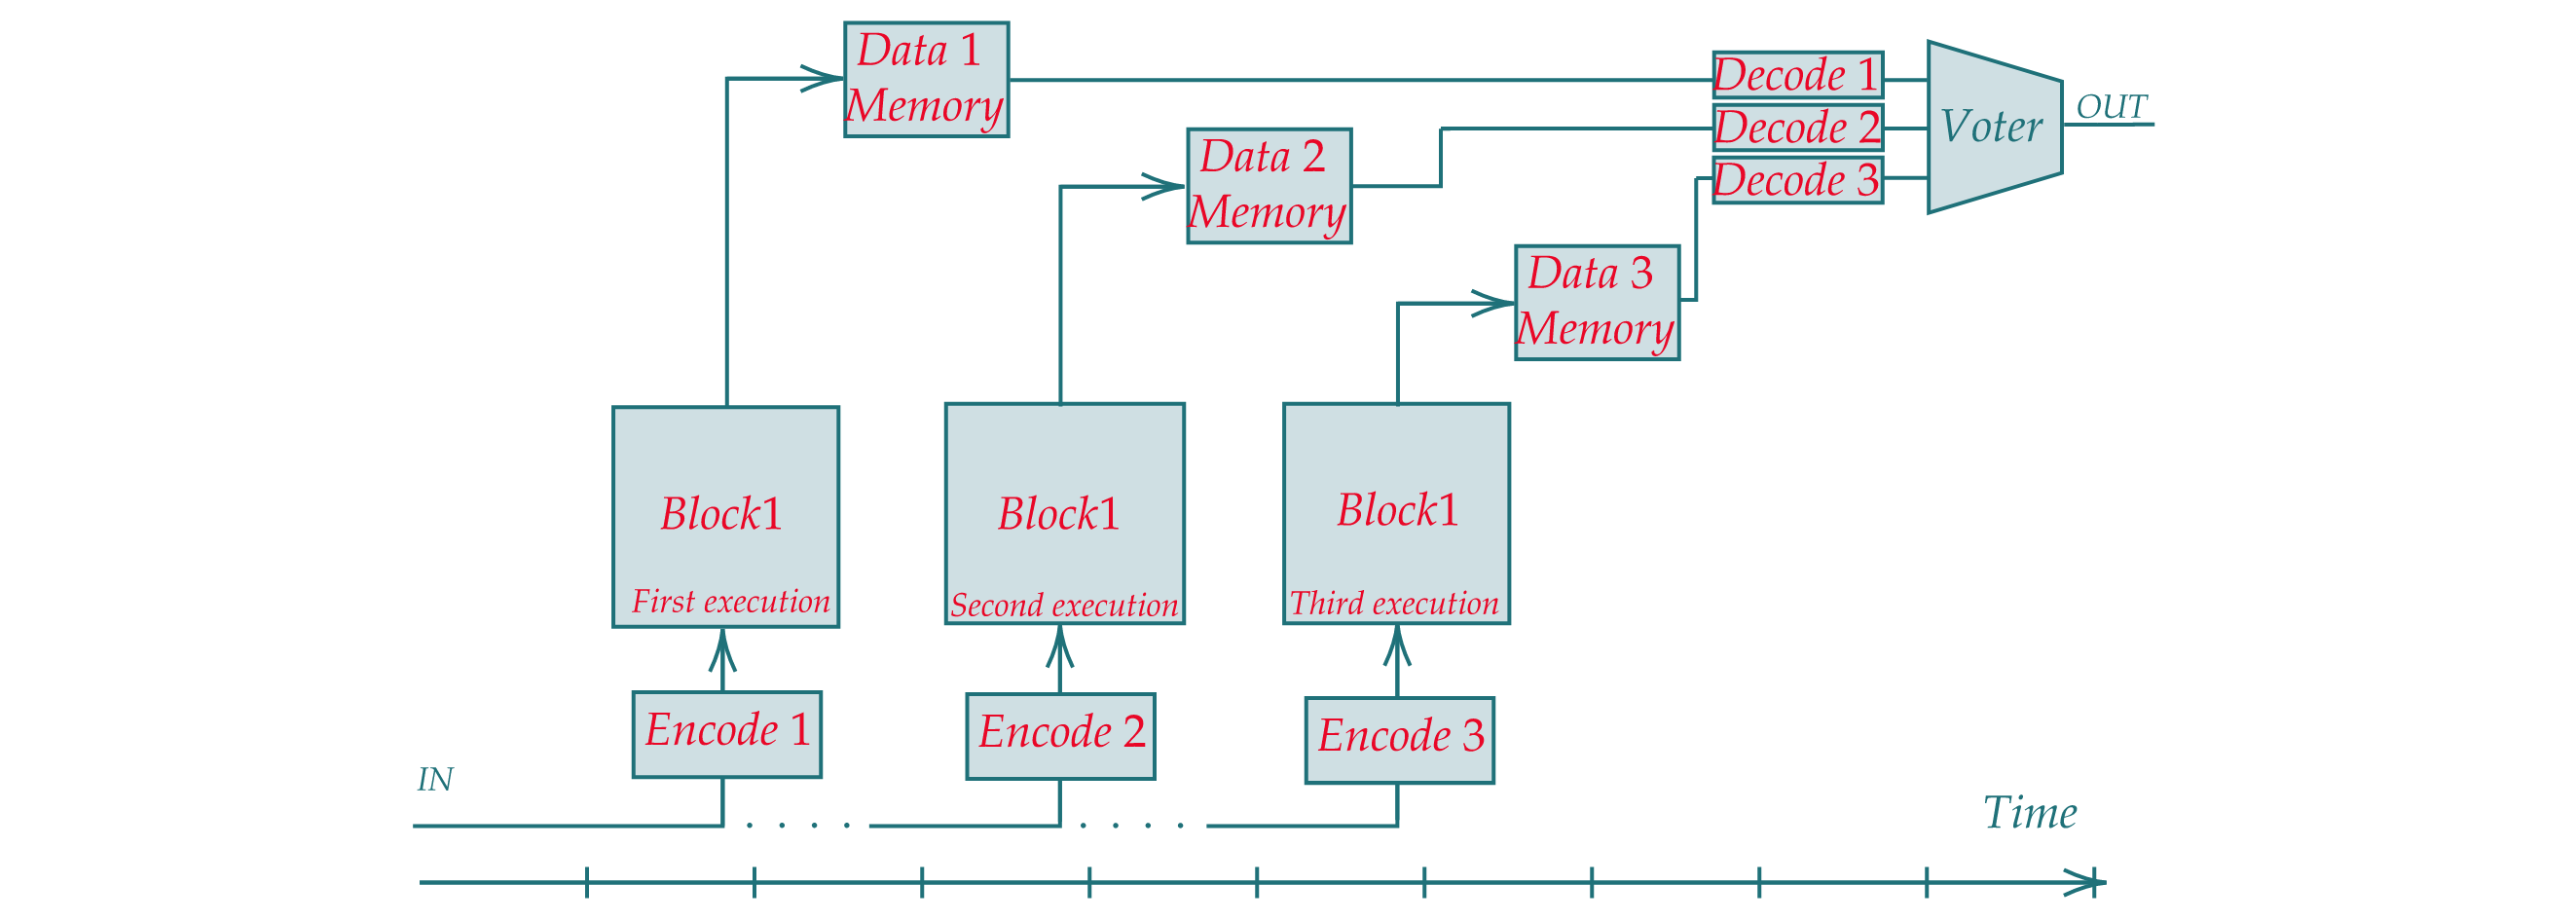
\includegraphics[scale=0.2,center]{./images/TimeRedundancy2.png}
    			\caption{Example of generic Temporal Redundancy with data encoding.}
    			\label{fig:TemporalRedundancy2}
    		\end{figure} 
			
			
		}
	
	
	    All previous techniques can be applied together and in mixed way in order to increase Reliability and MTTF of the overall system. 
	    The implementation of these techniques should be done considering power, area, performance and safety requirements. 
	    This trade off led to refine the techniques used to decide where and when use a specific protection, for example a 2012 research \bscite{Optimization_of_a_Cascading_TMR_system_configuration_using_Genetic_Algorithm}  investigate the use of genetic algorithm to find the best TMR configuration, in this case the triplication of blocks or/and voters is done in order to optimize area and reliability. \\
	    
	    A 2010 work create a software supported frame-work that is able to improve the TMR application basing on the temperature change in the chip, the methods consist in the application of TMR to all processor, then the core is Place and Route to FPGA and the temperature distribution is analyzed. Since temperature distribution give guidelines about where it is most likely faults to occur, it is possible to eliminate redundancy from parts of the design that operate under low temperatures without affecting fault masking. 
	    
	    
	} % end Hardening techniques for digital circuit architectures
	\section{Validation techniques for digital circuit architectures}{
		% Article & books
		%	
		\subsection{Real life testing}{
			% Article & books
			%	
			
		}
		\subsection{Ground Accelerated Radiation testing}{
			% Article & books
			%	7
			
		}
		\subsection{Analytical approach}{
			% Article & books
			% Simulation techniques chapter 9 : (book) Fault tolerant Systems
			
		}
		\subsection{Fault Injection (FI)}{
			% Article & books
			% soft error in Moder Electronic system chapter 6 and 7
			% Simulation techniques chapter 9 : (book) Fault tolerant Systems
			% Fault‐Injection Techniques chapter 7: Fault‐Tolerance Techniques for Spacecraft Control Computers
			
		}
	}
}